\chapter{约束优化与对偶}
\label{chap:constrained-optimization}

设想把两项预算分给两个项目：理想分配是$\bm c=(2,1)^\top$，但总额不能超过$\tau=2$，每项也不能为负。在“离理想分配最近”的意义下求解，就是最小化$\frac12\lVert\bm x-\bm c\rVert_2^2$，约束为$x_1+x_2\leq2$、$\bm x\geq\bm0$。目标的普通最小点$\bm c$越过了预算线，从任何可行点出发沿负梯度走一步也可能越界。答案是$\bm x^\star=(3/2,1/2)^\top$，可它的梯度$\bm x^\star-\bm c=(-1/2,-1/2)^\top$并不为零。于是几个问题同时出现：不能再用“梯度为零”判断最优时，怎样判断一个边界点是解？如果预算从$2$增加到$2.1$，最优值会下降多少？怎样计算这样的解，又怎样向别人证明所给答案离最优值不远？

本章的学习目标，是在有限维的等式、不等式和矩阵约束下回答这四个问题。我们要能写出并检验约束最优点必须满足的条件，构造给出目标下界的对偶问题，用原始—对偶两侧的界认证结果；要能区分最优值和最优解对数据变化的不同响应；要能辨认二次规划、二阶锥规划和半正定规划这些常用模型；还要掌握几类求解机制：保持迭代点可行、给违约计价、调整乘子、求局部二次模型、沿可行域内部的路径前进，以及先放宽非凸问题再恢复原解。

路线由这些问题的依赖关系决定。约束最优条件先从可行方向出发，只用集合本身描述最优性，再在约束资格成立时换成约束梯度和乘子；乘子随后成为构造下界的价格，对偶函数、凸共轭与强对偶回答下界何时紧。同一组乘子又给出最优值对约束右端的斜率，所以敏感性分析紧接在对偶之后。辨认出二次与锥模型以后，算法才有明确的对象：投影、条件梯度和镜像下降各用一种子问题保持可行；惩罚法和乘子法允许暂时违约，再用罚参数或乘子把迭代拉回可行域；序列二次规划和内点法则借用第~\ref{chap:opt-smooth}章的牛顿模型。最后，半正定松弛把一类非凸二次问题放宽成前面已经会解的凸问题，再讨论怎样从松弛解回到原问题。

\section{可行方向与约束最优条件}
\label{sec:opt-con-optimality}

第~\ref{chap:optimization}章证明了：可微目标在开集内部的局部最小点处梯度为零。章首的预算例说明，这条结论在可行域边界上失效，因为边界点附近并非每个方向都能走。本节先只用可行域本身描述“哪些方向能走、沿这些方向目标不能下降”，得到不依赖约束写法的最优条件；再在约束函数满足适当正则条件时，把这一条件改写成约束梯度与乘子的代数关系，即KKT条件。

全章讨论的一般问题是
\begin{equation}
\label{eq:opt-con-problem}
  \min_{\bm x\in\mathbb R^d}f(\bm x)
  \quad\text{s.t.}\quad
  g_i(\bm x)\leq0\ (i=1,\dots,m),\qquad
  h_j(\bm x)=0\ (j=1,\dots,p),
\end{equation}
可行域记为$C=\{\bm x:g_i(\bm x)\leq0,\ h_j(\bm x)=0\}$，最优值$f^\star=\inf_{\bm x\in C}f(\bm x)$。对可行点$\bm x$，满足$g_i(\bm x)=0$的约束称为\term{活跃约束}（active constraint），其下标集合记为$I(\bm x)$；$g_i(\bm x)<0$的约束在$\bm x$附近不起限制作用。本章反复使用两个小例子。

\begin{example}[等式二次例]
\label{ex:opt-con-equality-qp}
最小化$f(\bm x)=\frac12(x_1^2+4x_2^2)$，约束$h(\bm x)=x_1+x_2-1=0$。目标的等值线是以原点为中心、横向拉长的椭圆，可行域是一条直线。
\end{example}

\begin{example}[预算分配例]
\label{ex:opt-con-budget}
给定$\tau>0$，最小化$f(\bm x)=\frac12\lVert\bm x-\bm c\rVert_2^2$，$\bm c=(2,1)^\top$，约束为$g_1(\bm x)=x_1+x_2-\tau\leq0$、$g_2(\bm x)=-x_1\leq0$、$g_3(\bm x)=-x_2\leq0$。可行域是三角形，最优点是$\bm c$在三角形上的最近点。
\end{example}

\subsection{可行方向与法向量}
\label{sec:opt-con-feasible-directions}

\paragraph{凸可行域上的变分不等式}
先设可行域$C$是凸集。站在可行点$\bm x$上，若另一点$\bm y\in C$，凸性保证线段$\bm x+t(\bm y-\bm x)$（$0\leq t\leq1$）都在$C$中，所以$\bm y-\bm x$是一个可以走的方向。局部最小点不允许沿任何这样的方向一阶下降，这给出下面的条件。

\begin{theorem}[凸可行域上的一阶条件]
\label{thm:opt-con-variational-inequality}
设$C\subseteq\mathbb R^d$非空凸，$f$在包含$C$的开集上可微。若$\bm x^\star$是$f$在$C$上的局部最小点，则
\begin{equation}
\label{eq:opt-con-vi}
  \langle\nabla f(\bm x^\star),\bm y-\bm x^\star\rangle\geq0\qquad\text{对所有}\ \bm y\in C.
\end{equation}
若$f$还在$C$上凸，则式~\eqref{eq:opt-con-vi}也是$\bm x^\star$为全局最小点的充分条件。
\end{theorem}

\begin{proof}
固定$\bm y\in C$，令$\varphi(t)=f(\bm x^\star+t(\bm y-\bm x^\star))$。$t\in[0,1]$时自变量在$C$中，且$t$足够小时它落在$\bm x^\star$的比较邻域内，所以$\varphi(t)\geq\varphi(0)$。于是右导数$\varphi'(0^+)=\langle\nabla f(\bm x^\star),\bm y-\bm x^\star\rangle\geq0$。若$f$凸，第~\ref{chap:optimization}章的一阶支撑下界给出$f(\bm y)\geq f(\bm x^\star)+\langle\nabla f(\bm x^\star),\bm y-\bm x^\star\rangle\geq f(\bm x^\star)$。
\end{proof}

式~\eqref{eq:opt-con-vi}称为一阶\term{变分不等式}（variational inequality）。它把“不能下降”写成对全部可行方向的检验：梯度可以不为零，但它必须与每个可行方向成不超过直角的夹角。把这个要求从梯度一侧改写到集合一侧，就得到法锥。

\begin{definition}[法锥]
\label{def:opt-con-normal-cone}
设$C$非空凸，$\bm x\in C$。集合
\[
  N_C(\bm x)=\{\bm v\in\mathbb R^d:\langle\bm v,\bm y-\bm x\rangle\leq0\ \text{对所有}\ \bm y\in C\}
\]
称为$C$在$\bm x$处的\term{法锥}（normal cone）。
\end{definition}

法锥中的向量与所有从$\bm x$出发的可行弦成钝角或直角，是“指向集合外侧”的方向；它对非负倍数和加法封闭，所以是凸锥。用这个记号，式~\eqref{eq:opt-con-vi}就是$-\nabla f(\bm x^\star)\in N_C(\bm x^\star)$：最优点处，下降最快的方向必须指向可行域外。

\paragraph{内点、光滑边界与角点}
法锥的大小随点的位置变化。图~\ref{fig:opt-con-normal-cone}在预算分配例（$\tau=2$）中改变理想分配$\bm c$，依次得到三种情形。若$\bm c=(0.6,0.8)^\top$在三角形内部，最近点就是$\bm c$本身；内点处每个方向都可行，法锥只有零向量，条件退回为$\nabla f(\bm x^\star)=\bm0$。若$\bm c=(2,1)^\top$，最近点$\bm x^\star=(3/2,1/2)^\top$位于斜边内部，法锥是斜边外法向$(1,1)^\top$的非负倍数；此时$-\nabla f(\bm x^\star)=\bm c-\bm x^\star=\frac12(1,1)^\top$正好在这条射线上。若$\bm c=(3,-1)^\top$，最近点是角点$(2,0)^\top$，法锥由两条边的外法向$(1,1)^\top$和$(0,-1)^\top$张成，$-\nabla f=(1,-1)^\top=1\cdot(1,1)^\top+2\cdot(0,-1)^\top$落在锥内。角点处可以直接验证式~\eqref{eq:opt-con-vi}：对三角形中任意$\bm y$，$\langle(1,-1)^\top,\bm y-(2,0)^\top\rangle=y_1-y_2-2\leq y_1+y_2-2\leq0$，其中用了$y_2\geq0$与$y_1+y_2\leq2$。

\begin{figure*}[!htbp]
  \centering
  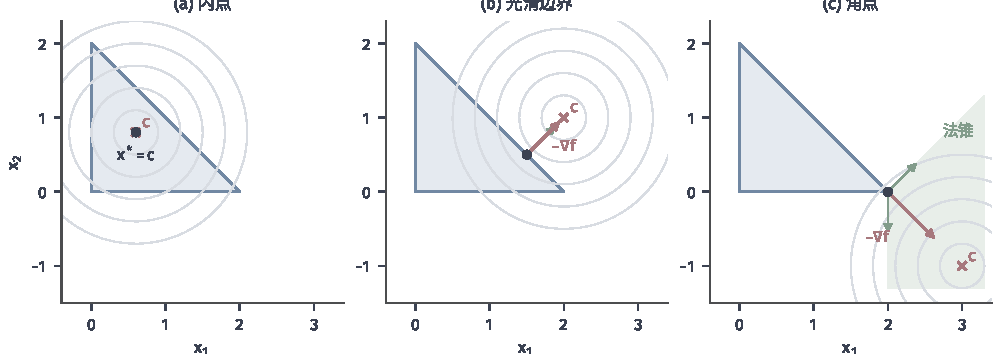
\includegraphics[width=169mm]{figures/03-optimization-evolution-and-signals/01-optimization/matplotlib/c5-normal-cone/figure.pdf}
  \caption{预算分配例（$\tau=2$）中最近点与法锥。浅蓝三角形为可行域，灰色圆为目标$\frac12\lVert\bm x-\bm c\rVert_2^2$的等值线，红叉为理想分配$\bm c$，黑点为最优点。(a) $\bm c$在内部，最优点处梯度为零；(b) 最优点在斜边上，红色箭头$-\nabla f$与绿色外法向同向；(c) 最优点在角点，绿色区域是两条外法向张成的法锥，$-\nabla f=(1,-1)^\top$落在其中。}
  \label{fig:opt-con-normal-cone}
\end{figure*}

三种情形说明，边界最优点的梯度通常不为零；判断最优性要看负梯度是否落在法锥中。光滑边界上的法锥是一条射线，角点处的法锥是一块锥形区域，因此角点能“容纳”更多方向的负梯度，这也是线性规划的解常落在顶点上的几何原因。

\paragraph{非线性约束：真实方向与线性化方向}
可行域由非线性约束给出时，它一般不是凸集，从$\bm x$出发的直线段可能立刻离开$C$。真实能走的方向要用可行点列来描述：若存在可行点$\bm x^{(k)}\to\bm x$和正数$t_k\downarrow0$，使$(\bm x^{(k)}-\bm x)/t_k\to\bm d$，就称$\bm d$属于$C$在$\bm x$处的\term{切锥}（contingent cone），记为$T_C(\bm x)$。它是闭锥，其中的方向可以由曲线或点列逼近，不必是直线段。

\begin{theorem}[切锥上的一阶必要条件]
\label{thm:opt-con-tangent-necessary}
设$f$在$\bm x^\star$附近可微，$\bm x^\star$是$f$在$C$上的局部最小点，则$\langle\nabla f(\bm x^\star),\bm d\rangle\geq0$对所有$\bm d\in T_C(\bm x^\star)$成立。
\end{theorem}

\begin{proof}
取$\bm d\in T_C(\bm x^\star)$及相应的$\bm x^{(k)}$、$t_k$。$k$足够大时$\bm x^{(k)}$落在比较邻域内，由Taylor展开，
\[
  0\leq\frac{f(\bm x^{(k)})-f(\bm x^\star)}{t_k}
  =\Bigl\langle\nabla f(\bm x^\star),\frac{\bm x^{(k)}-\bm x^\star}{t_k}\Bigr\rangle+\frac{o(\lVert\bm x^{(k)}-\bm x^\star\rVert_2)}{t_k}.
\]
由于$\lVert\bm x^{(k)}-\bm x^\star\rVert_2/t_k$有界，最后一项趋于零；令$k\to\infty$即得结论。
\end{proof}

切锥由可行域的几何决定，直接计算往往困难。实际可用的是约束函数的一阶近似：把活跃约束线性化，得到
\[
  L(\bm x)=\{\bm d:\langle\nabla h_j(\bm x),\bm d\rangle=0\ (\text{全部}\ j),\ \langle\nabla g_i(\bm x),\bm d\rangle\leq0\ (i\in I(\bm x))\},
\]
其中的方向称为\term{线性化可行方向}（linearized feasible direction）。真实方向总是线性化允许的：若$\bm d\in T_C(\bm x)$，对活跃的$g_i$有$0\geq g_i(\bm x^{(k)})-g_i(\bm x)=\langle\nabla g_i(\bm x),\bm x^{(k)}-\bm x\rangle+o(\lVert\bm x^{(k)}-\bm x\rVert_2)$，除以$t_k$再取极限得$\langle\nabla g_i(\bm x),\bm d\rangle\leq0$；等式约束同理得到等号。因此$T_C(\bm x)\subseteq L(\bm x)$。

反向包含可能不成立。图~\ref{fig:opt-con-cusp}中的可行域由$g_1(\bm x)=x_2-(1-x_1)^3\leq0$与$g_2(\bm x)=-x_2\leq0$给出，在$(1,0)^\top$处形成一个尖点。两条约束在该点都活跃，梯度分别为$(0,1)^\top$和$(0,-1)^\top$，线性化只要求$d_2=0$，于是$(1,0)^\top$和$(-1,0)^\top$都被允许；但当$x_1>1$时$(1-x_1)^3<0\leq x_2$，没有可行点，真实切锥只有$\{(-t,0)^\top:t\geq0\}$。线性化把一条不存在的方向当成了可行方向。取$f(\bm x)=-x_1$，点$(1,0)^\top$是全局最小点，满足定理~\ref{thm:opt-con-tangent-necessary}；可是线性化方向$(1,0)^\top$上$\langle\nabla f,\bm d\rangle=-1<0$，若只看线性化模型，会误以为还能下降。

\begin{figure}[!htbp]
  \centering
  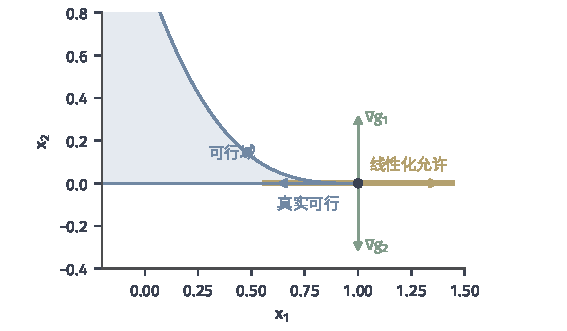
\includegraphics[width=96mm]{figures/03-optimization-evolution-and-signals/01-optimization/matplotlib/c5-cusp/figure.pdf}
  \caption{尖点处线性化方向多于真实方向。浅蓝区域为$x_2\leq(1-x_1)^3$且$x_2\geq0$的可行域，黑点为$(1,0)^\top$，绿色箭头为两条活跃约束的梯度。黄色线段表示线性化允许的方向$d_2=0$（左右两侧都允许），蓝色箭头是唯一真实可行的方向$(-1,0)^\top$。}
  \label{fig:opt-con-cusp}
\end{figure}

因此，从切锥上的必要条件过渡到只含约束梯度的条件，需要一个保证$T_C(\bm x)=L(\bm x)$的正则条件。下一小节先在这一条件下推出乘子，再用这个尖点说明条件缺失时乘子确实可能不存在。

\subsection{Lagrange乘子与KKT条件}
\label{sec:opt-con-kkt}

\paragraph{等式约束：梯度落在法向张成中}
图~\ref{fig:opt-con-tangency}画出等式二次例。沿约束直线移动时，目标值先降后升；在最优点，直线恰好与一条等值线相切。相切意味着梯度与直线的切向量$(1,-1)^\top$正交，即$\nabla f(\bm x^\star)$与约束的法向$\nabla h=(1,1)^\top$平行，可写成$\nabla f(\bm x^\star)+\nu\nabla h(\bm x^\star)=\bm0$，其中$\nu$是一个待定实数。这个系数称为\term{拉格朗日乘子}（Lagrange multiplier）。

\begin{figure}[!htbp]
  \centering
  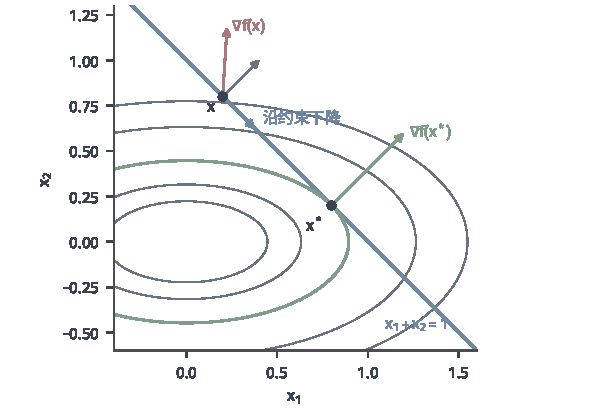
\includegraphics[width=100mm]{figures/03-optimization-evolution-and-signals/01-optimization/matplotlib/c5-tangency/figure.pdf}
  \caption{等式二次例的切点条件。灰色椭圆为$f(\bm x)=\frac12(x_1^2+4x_2^2)$的等值线，蓝线为约束$x_1+x_2=1$。在最优点$\bm x^\star=(4/5,1/5)^\top$，绿色等值线与约束线相切，梯度$(4/5,4/5)^\top$垂直于约束线。在非最优可行点$\bm x=(0.2,0.8)^\top$，红色梯度$(0.2,3.2)^\top$有沿约束线的分量，蓝色箭头所示的切向负分量仍能降低目标。}
  \label{fig:opt-con-tangency}
\end{figure}

在这个例子中，$\nabla f=(x_1,4x_2)^\top$，方程组$x_1+\nu=0$、$4x_2+\nu=0$、$x_1+x_2=1$给出$x_1=-\nu$、$x_2=-\nu/4$，代入约束得$-\frac54\nu=1$，所以$\nu^\star=-4/5$，$\bm x^\star=(4/5,1/5)^\top$，$f^\star=\frac12(16/25+4/25)=2/5$。对照非最优点$(0.2,0.8)^\top$：梯度$(0.2,3.2)^\top$在切向$(1,-1)^\top/\sqrt2$上的分量为$-3/\sqrt2\neq0$，沿$(1,-1)^\top$移动会降低目标，所以它不满足平行条件。

\paragraph{加入不等式：乘子的符号与互补松弛}
不等式约束只在活跃时限制移动，而且只限制向外的一侧。最优点处，负梯度应能写成活跃约束外法向的非负组合，这就是法锥的代数形式。以预算分配例（$\tau=2$）为例，最优点$\bm x^\star=(3/2,1/2)^\top$只使$g_1$活跃，$\nabla f(\bm x^\star)=(-1/2,-1/2)^\top$，取$\lambda_1=1/2$便有$\nabla f+\lambda_1\nabla g_1=\bm0$；未活跃的$g_2,g_3$取零乘子。若把$\bm c$换成$(3,-1)^\top$，最优点$(2,0)^\top$使$g_1,g_3$同时活跃，由$(-1,1)^\top+\lambda_1(1,1)^\top+\lambda_3(0,-1)^\top=\bm0$解出$\lambda_1=1$、$\lambda_3=2$，正是图~\ref{fig:opt-con-normal-cone}(c)中的分解。可以把$\lambda_i\nabla g_i$看成第$i$条约束施加的“反作用力”：目标推着点向$-\nabla f$方向走，活跃约束只能沿外法向往回推，且推力非负；最优点处各力平衡。

把等式与不等式合在一起，引入
\begin{equation}
\label{eq:opt-con-lagrangian}
  \mathcal L(\bm x,\bm\lambda,\bm\nu)=f(\bm x)+\sum_{i=1}^m\lambda_ig_i(\bm x)+\sum_{j=1}^p\nu_jh_j(\bm x),
\end{equation}
称为\term{拉格朗日函数}（Lagrangian）。“未活跃约束乘子为零”可以写成乘积$\lambda_ig_i(\bm x)=0$，这样就不必事先知道哪些约束活跃。

\begin{definition}[KKT条件]
\label{def:opt-con-kkt}
设$f,g_i,h_j$在$\bm x^\star$处可微。若存在$\bm\lambda^\star\in\mathbb R^m$、$\bm\nu^\star\in\mathbb R^p$，使
\begin{align*}
  &\text{驻点性：}&&\nabla f(\bm x^\star)+\textstyle\sum_i\lambda_i^\star\nabla g_i(\bm x^\star)+\sum_j\nu_j^\star\nabla h_j(\bm x^\star)=\bm0,\\
  &\text{原始可行性：}&&g_i(\bm x^\star)\leq0,\quad h_j(\bm x^\star)=0,\\
  &\text{对偶可行性：}&&\lambda_i^\star\geq0,\\
  &\text{互补松弛：}&&\lambda_i^\star g_i(\bm x^\star)=0\quad(i=1,\dots,m),
\end{align*}
就称$(\bm x^\star,\bm\lambda^\star,\bm\nu^\star)$满足\term{Karush--Kuhn--Tucker条件}（KKT conditions），简称KKT点。
\end{definition}

四组条件分工不同。驻点性就是$\nabla_{\bm x}\mathcal L=\bm0$，表达力的平衡；原始可行性保证候选满足约束；对偶可行性规定不等式乘子的方向；\term{互补松弛}（complementary slackness）规定只有活跃约束可以带正乘子。等式乘子没有符号限制，因为等式约束两侧都不能越过。互补松弛只说“乘子为正则约束活跃”，反过来不成立：预算分配例取$\tau=3$时，最优点$(2,1)^\top=\bm c$使预算约束恰好活跃，乘子却是零，因为目标本身已经不想越过预算线。

\paragraph{乘子存在所需的约束资格}
KKT条件是从局部最优推出来的必要条件，但这一推导需要条件。以下最常用的条件要求活跃约束的梯度彼此独立。

\begin{definition}[线性无关约束资格]
\label{def:opt-con-licq}
若全部$\nabla h_j(\bm x)$与活跃的$\nabla g_i(\bm x)$（$i\in I(\bm x)$）线性无关，就说可行点$\bm x$满足\term{线性无关约束资格}（linear independence constraint qualification，LICQ）。LICQ是一种\term{约束资格条件}（constraint qualification）。
\end{definition}

\begin{theorem}[LICQ下KKT条件的必要性]
\label{thm:opt-con-kkt-necessary}
设$f,g_i,h_j$在$\bm x^\star$的邻域内连续可微，$\bm x^\star$是问题~\eqref{eq:opt-con-problem}的局部最小点且满足LICQ，则存在唯一的$(\bm\lambda^\star,\bm\nu^\star)$使KKT条件成立。
\end{theorem}

\begin{proof}
记$\bm E$为以$\nabla h_j(\bm x^\star)^\top$为行的矩阵，$\bm B$为以活跃$\nabla g_i(\bm x^\star)^\top$为行的矩阵。

\emph{第一步：线性化方向都是真实方向。}LICQ说明$\begin{bmatrix}\bm E\\\bm B\end{bmatrix}$行满秩，故方程$\bm E\bar{\bm d}=\bm0$、$\bm B\bar{\bm d}=-\bm 1$有解$\bar{\bm d}$。先取严格方向$\bm d$，即$\bm E\bm d=\bm0$、$\bm B\bm d<\bm0$。考虑方程$\bm h(\bm x^\star+t\bm d+\bm E^\top\bm w)=\bm0$，未知量为$\bm w\in\mathbb R^p$；它在$(t,\bm w)=(0,\bm0)$成立，关于$\bm w$的Jacobian为$\bm E\bm E^\top$，由LICQ可逆。隐函数定理给出$t$附近的连续可微解$\bm w(t)$，$\bm w(0)=\bm0$，且$\bm w'(0)=-(\bm E\bm E^\top)^{-1}\bm E\bm d=\bm0$。曲线$\bm x(t)=\bm x^\star+t\bm d+\bm E^\top\bm w(t)$满足全部等式约束，且$\bm x(t)=\bm x^\star+t\bm d+o(t)$。对活跃的$g_i$，$g_i(\bm x(t))=t\langle\nabla g_i(\bm x^\star),\bm d\rangle+o(t)<0$；未活跃的$g_i$由连续性在$t$小时仍为负。所以$\bm x(t)$在小$t>0$时可行，$\bm d\in T_C(\bm x^\star)$。对一般$\bm d\in L(\bm x^\star)$，$\bm d+\varepsilon\bar{\bm d}$对每个$\varepsilon>0$都是严格方向，而切锥是闭集，令$\varepsilon\downarrow0$得$\bm d\in T_C(\bm x^\star)$。于是$T_C(\bm x^\star)=L(\bm x^\star)$。

\emph{第二步：由择一定理得到乘子。}由定理~\ref{thm:opt-con-tangent-necessary}，不存在$\bm d$使$\bm E\bm d=\bm0$、$\bm B\bm d\leq\bm0$且$\langle\nabla f(\bm x^\star),\bm d\rangle<0$。第~\ref{chap:opt-linear-programming}章的Farkas择一定理说：对矩阵$\bm M$和向量$\bm r$，系统$\bm M\bm u=\bm r,\ \bm u\geq\bm0$与系统$\bm M^\top\bm z\geq\bm0,\ \bm r^\top\bm z<0$恰有一个可行。取$\bm M=[\bm B^\top,\ \bm E^\top,\ -\bm E^\top]$、$\bm r=-\nabla f(\bm x^\star)$。若第二个系统有解$\bm z$，则$\bm d=-\bm z$满足$\bm B\bm d\leq\bm0$、$\bm E\bm d=\bm0$和$\langle\nabla f(\bm x^\star),\bm d\rangle=\bm r^\top\bm z<0$，与上面矛盾。所以第一个系统有解$\bm u=(\bm\lambda_I,\bm\nu^+,\bm\nu^-)\geq\bm0$，即$-\nabla f(\bm x^\star)=\bm B^\top\bm\lambda_I+\bm E^\top(\bm\nu^+-\bm\nu^-)$。令$\bm\nu^\star=\bm\nu^+-\bm\nu^-$，活跃乘子取$\bm\lambda_I$，未活跃乘子取零，四组KKT条件全部成立。乘子唯一，因为两组乘子之差会给出活跃梯度的一个非零线性组合等于零，与LICQ矛盾。
\end{proof}

回到尖点：在$(1,0)^\top$处两条活跃梯度$(0,1)^\top$与$(0,-1)^\top$线性相关，LICQ不成立。驻点方程$(-1,0)^\top+\lambda_1(0,1)^\top+\lambda_2(0,-1)^\top=\bm0$的第一个分量是$-1=0$，无解；最小点存在，乘子却不存在。更简单的例子是$\min x$、约束$x^2\leq0$：唯一可行点$0$是最小点，但$\nabla g(0)=0$，驻点方程$1+\lambda\cdot0=0$无解。LICQ只是约束资格的一种；凸问题中常用的Slater条件将在第~\ref{sec:opt-con-duality}节出现。

\paragraph{凸问题中KKT条件的充分性}
必要性回答“最优点是否一定有乘子”；反过来，已经拿到一组满足KKT条件的候选时，需要知道它是不是全局最优。凸结构给出肯定的回答，而且不需要任何约束资格。

\begin{theorem}[凸问题的KKT充分性]
\label{thm:opt-con-kkt-sufficient}
设$f$与各$g_i$是可微凸函数，各$h_j$是仿射函数。若$(\bm x^\star,\bm\lambda^\star,\bm\nu^\star)$满足KKT条件，则$\bm x^\star$是问题~\eqref{eq:opt-con-problem}的全局最小点。
\end{theorem}

\begin{proof}
固定乘子，函数$\bm x\mapsto\mathcal L(\bm x,\bm\lambda^\star,\bm\nu^\star)$是凸函数的非负组合加仿射函数，因而凸；驻点性说明它在$\bm x^\star$处梯度为零，所以$\bm x^\star$是它的全局最小点。对任意可行$\bm x$，$\lambda_i^\star g_i(\bm x)\leq0$、$h_j(\bm x)=0$，于是
\[
  f(\bm x)\geq\mathcal L(\bm x,\bm\lambda^\star,\bm\nu^\star)\geq\mathcal L(\bm x^\star,\bm\lambda^\star,\bm\nu^\star)=f(\bm x^\star),
\]
最后的等号用了互补松弛和$h_j(\bm x^\star)=0$。
\end{proof}

预算分配例的目标凸、约束仿射，所以前面算出的$\bm x^\star=(3/2,1/2)^\top$连同乘子$\lambda_1=1/2$已经证明了全局最优，无需再检查约束资格。非凸问题中KKT条件只是候选检验：在$[-1,1]$上最小化$f(x)=-x^2$，约束写成$x-1\leq0$、$-x-1\leq0$，点$x=0$不使任何约束活跃，驻点性$-2x=0$成立，乘子全取零便满足KKT条件，但它是全局最大点；真正的最小点$x=\pm1$也满足KKT条件，例如$x=1$处取$\lambda_1=2$。在非凸问题里，KKT条件筛掉的是明显不合格的点，留下的候选还需要比较目标值或用其他论证区分。

\section{对偶问题与最优性证书}
\label{sec:opt-con-duality}

KKT条件检验的是一个候选点，回答“它是否满足最优点应有的关系”。实际求解时还需要另一种回答：给定一个可行点，它的目标值离最优值最多差多少。可行点只给出最优值的上界，要控制差距，必须另有下界。上一节的乘子正好能产生下界：把约束乘以合法乘子加进目标，就得到一个在可行域上不超过原目标的函数。本节固定原问题，研究这种下界怎样构造、什么时候能一直提高到原最优值，以及怎样把原始和对偶两侧的候选合成一份证书；问题数据改变时最优值怎样变化，放到下一节讨论。

\subsection{对偶函数与弱对偶}
\label{sec:opt-con-weak-duality}

\paragraph{先对原变量取下确界}
固定$\bm\lambda\geq\bm0$和任意$\bm\nu$。对每个可行点$\bm x$，$\lambda_ig_i(\bm x)\leq0$、$h_j(\bm x)=0$，所以$\mathcal L(\bm x,\bm\lambda,\bm\nu)\leq f(\bm x)$。如果再对全体$\bm x\in\mathbb R^d$（不论是否可行）取下确界，得到的数不会超过任何可行点的目标值。

\begin{definition}[对偶函数与对偶问题]
\label{def:opt-con-dual-function}
问题~\eqref{eq:opt-con-problem}的\term{对偶函数}（dual function）为
\[
  q(\bm\lambda,\bm\nu)=\inf_{\bm x\in\mathbb R^d}\mathcal L(\bm x,\bm\lambda,\bm\nu),
\]
允许取$-\infty$。称$\max\{q(\bm\lambda,\bm\nu):\bm\lambda\geq\bm0\}$为\term{对偶问题}（dual problem），其最优值记为$d^\star=\sup_{\bm\lambda\geq\bm0,\bm\nu}q(\bm\lambda,\bm\nu)$。满足$\bm\lambda\geq\bm0$且$q(\bm\lambda,\bm\nu)>-\infty$的乘子称为对偶可行。
\end{definition}

对每个固定的$\bm x$，$\mathcal L(\bm x,\cdot,\cdot)$是乘子的仿射函数；$q$是这族仿射函数的逐点下确界，因而无论原问题是否凸，$q$总是凹函数，对偶问题总是凸问题。

\begin{theorem}[弱对偶]
\label{thm:opt-con-weak-duality}
对任意可行$\bm x$与任意$\bm\lambda\geq\bm0$、$\bm\nu$，有$q(\bm\lambda,\bm\nu)\leq f(\bm x)$。因而$d^\star\leq f^\star$。
\end{theorem}

\begin{proof}
$q(\bm\lambda,\bm\nu)\leq\mathcal L(\bm x,\bm\lambda,\bm\nu)\leq f(\bm x)$，第一步是下确界的定义，第二步是上面的符号论证。对可行$\bm x$取下确界、对乘子取上确界即得$d^\star\leq f^\star$。
\end{proof}

\term{弱对偶}（weak duality）不需要凸性、可微性或约束资格。两值都有限时，差$f^\star-d^\star\geq0$称为\term{对偶间隙}（duality gap）。

\paragraph{一个可以画出来的下界}
考虑$\min x^2$、约束$g(x)=1-x\leq0$，最优点$x^\star=1$，$f^\star=1$。$\mathcal L(x,\lambda)=x^2+\lambda(1-x)$在$x=\lambda/2$处取最小，于是$q(\lambda)=\lambda-\lambda^2/4$，在$\lambda=2$处达到$d^\star=1=f^\star$。图~\ref{fig:opt-con-dual-envelope}给出这个计算的几何含义。把每个$x$映成平面点$(u,t)=(g(x),f(x))$，得到曲线$G$；对固定的$\lambda$，$\mathcal L=t+\lambda u$在直线$t+\lambda u=\text{常数}$上不变，这族直线的斜率都是$-\lambda$。$q(\lambda)$就是把斜率为$-\lambda$的直线从下方推到刚好碰到$G$时，直线在$u=0$处的截距。原问题要求$u=g(x)\leq0$，最优值是$G$中$u\leq0$部分的最低高度；每条支撑直线在$u=0$处的截距都不超过它，这就是弱对偶。对偶问题在所有斜率中寻找截距最高的一条，本例中$\lambda=2$的直线恰好在$(0,1)$处与$G$相切。

\begin{figure*}[!htbp]
  \centering
  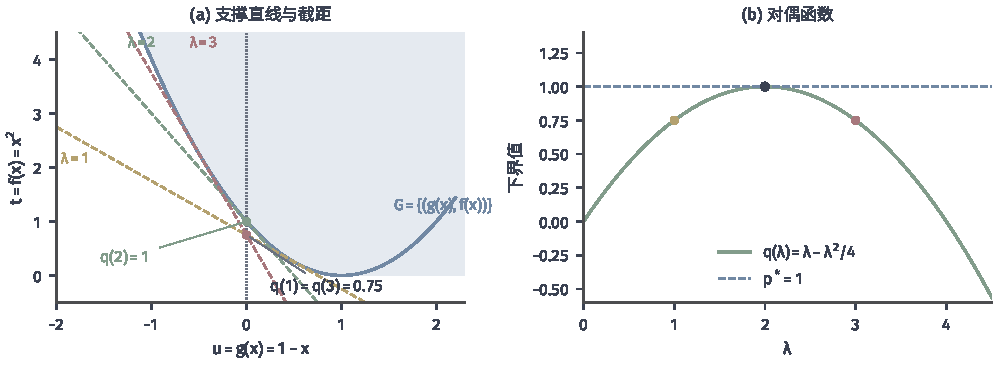
\includegraphics[width=169mm]{figures/03-optimization-evolution-and-signals/01-optimization/matplotlib/c5-dual-envelope/figure.pdf}
  \caption{$\min x^2$、$1-x\leq0$的对偶函数。(a) 蓝色曲线为$G=\{(1-x,x^2)\}$，浅蓝区域为其右上方的点；三条虚线是斜率为$-\lambda$（$\lambda=1,2,3$）且从下方接触$G$的直线，它们在$u=0$的截距即$q(\lambda)$。$\lambda=1$与$\lambda=3$的截距同为$0.75$，$\lambda=2$的截距为$1$，与原最优值相等。(b) 对偶函数$q(\lambda)=\lambda-\lambda^2/4$是凹函数，始终位于$f^\star=1$下方，最大值在$\lambda=2$处达到。}
  \label{fig:opt-con-dual-envelope}
\end{figure*}

在等式二次例中同样可以显式计算：$\mathcal L=\frac12(x_1^2+4x_2^2)+\nu(x_1+x_2-1)$在$x_1=-\nu$、$x_2=-\nu/4$处取最小，$q(\nu)=-\frac58\nu^2-\nu$，在$\nu^\star=-4/5$处达到$d^\star=2/5=f^\star$。对偶函数也可能处处为$-\infty$：在$[-1,1]$上最小化$-x^2$时，$\mathcal L=-x^2+\lambda_1(x-1)+\lambda_2(-x-1)$对任何乘子都没有下界，所以$d^\star=-\infty$，而$f^\star=-1$。某一组乘子给出$q=-\infty$，只说明这组乘子没有提供有用的下界。

\paragraph{近似内层只给出上方估计}
计算$q(\bm\lambda,\bm\nu)$本身是一个无约束最小化。若内层只算到近似点$\tilde{\bm x}$，那么$\mathcal L(\tilde{\bm x},\bm\lambda,\bm\nu)\geq q(\bm\lambda,\bm\nu)$，这个数在真正的下界上方，不能直接当作原问题的下界。要得到可靠下界，必须扣除一个经过证明的内层误差$\varepsilon$。例如$\mathcal L(\cdot,\bm\lambda,\bm\nu)$为$\mu$强凸时，对任意$\bm y$，
\[
  \mathcal L(\bm y)\geq\mathcal L(\tilde{\bm x})+\langle\nabla\mathcal L(\tilde{\bm x}),\bm y-\tilde{\bm x}\rangle+\frac\mu2\lVert\bm y-\tilde{\bm x}\rVert_2^2\geq\mathcal L(\tilde{\bm x})-\frac{1}{2\mu}\lVert\nabla\mathcal L(\tilde{\bm x})\rVert_2^2,
\]
最后一步对$\bm y$最小化右端的二次函数。于是$\mathcal L(\tilde{\bm x})-\lVert\nabla_{\bm x}\mathcal L(\tilde{\bm x})\rVert_2^2/(2\mu)$是可信下界。没有这类误差界时，近似内层值只能作为启发性估计。

\paragraph{原始—对偶间隙证书}
把两侧合起来，就得到可以交给别人核对的证书。若$\hat{\bm x}$可行、$(\bm\lambda,\bm\nu)$满足$\bm\lambda\geq\bm0$，则由弱对偶，
\begin{equation}
\label{eq:opt-con-gap-certificate}
  q(\bm\lambda,\bm\nu)\leq f^\star\leq f(\hat{\bm x}),\qquad
  0\leq f(\hat{\bm x})-f^\star\leq f(\hat{\bm x})-q(\bm\lambda,\bm\nu).
\end{equation}
右端可以计算，不需要知道$f^\star$。在等式二次例中取可行点$\hat{\bm x}=(3/4,1/4)^\top$与乘子$\nu=-3/4$：$f(\hat{\bm x})=0.40625$，$q(-3/4)=-\frac58\cdot\frac9{16}+\frac34=0.3984375$，间隙为$0.0078125$，所以$\hat{\bm x}$的次优性不超过$0.0079$；实际次优性为$0.40625-0.4=0.00625$。报告这样的证书时应分别给出三项：$\hat{\bm x}$的原始可行性（约束残差）、乘子的合法性（$\bm\lambda\geq\bm0$且$q$的计算可信），以及上下界之差。任何一项缺失，式~\eqref{eq:opt-con-gap-certificate}都不能使用。

第~\ref{chap:opt-linear-programming}章的线性规划对偶是这一构造的特例。对标准型$\min\bm c^\top\bm x$、$\bm A\bm x=\bm b$、$\bm x\geq\bm0$，把$-\bm x\leq\bm0$的乘子记为$\bm s\geq\bm0$、等式乘子记为$-\bm y$，则$\mathcal L=\bm c^\top\bm x-\bm y^\top(\bm A\bm x-\bm b)-\bm s^\top\bm x=\bm b^\top\bm y+(\bm c-\bm A^\top\bm y-\bm s)^\top\bm x$。关于$\bm x$的下确界有限当且仅当$\bm c-\bm A^\top\bm y-\bm s=\bm0$，此时$q=\bm b^\top\bm y$；消去$\bm s\geq\bm0$即得对偶问题$\max\bm b^\top\bm y$、$\bm A^\top\bm y\leq\bm c$。线性规划的特殊之处在于内层可以显式消去，本节保留的是同一个“用价格给目标作下界”的问题。

\subsection{凸共轭与对偶表示}
\label{sec:opt-con-conjugate}

对偶函数的计算核心是“目标加一个线性项后取下确界”。这一运算单独拿出来就是凸共轭。它把目标函数、约束集合与下方仿射函数联系起来，也为下一小节证明强对偶准备了工具。

\paragraph{用仿射函数从下方逼近}
设$f:\mathbb R^d\to\mathbb R\cup\{+\infty\}$。固定斜率$\bm y$，问：截距至少要降多少，仿射函数$\langle\bm y,\bm x\rangle-\beta$才能处处不超过$f$？条件是$\beta\geq\langle\bm y,\bm x\rangle-f(\bm x)$对所有$\bm x$成立，最小的$\beta$就是下面的上确界。

\begin{definition}[凸共轭]
\label{def:opt-con-conjugate}
函数$f$的\term{凸共轭}（convex conjugate）为$f^*(\bm y)=\sup_{\bm x\in\mathbb R^d}\{\langle\bm y,\bm x\rangle-f(\bm x)\}$，取值于$\mathbb R\cup\{+\infty\}$；$f(\bm x)=+\infty$的点不影响上确界。
\end{definition}

于是$\langle\bm y,\bm x\rangle-f^*(\bm y)$是斜率为$\bm y$的最高仿射下界，它的截距是$-f^*(\bm y)$。$f^*$是一族仿射函数（以$\bm x$为参数）的上确界，所以总是凸的，即使$f$不凸。由定义直接得到\term{Fenchel--Young不等式}（Fenchel--Young inequality）
\begin{equation}
\label{eq:opt-con-fenchel-young}
  f(\bm x)+f^*(\bm y)\geq\langle\bm x,\bm y\rangle\qquad\text{对所有}\ \bm x,\bm y.
\end{equation}

\begin{example}[几个基本共轭]
\label{ex:opt-con-conjugates}
(1) $f(x)=x^2/2$：$yx-x^2/2=y^2/2-(x-y)^2/2$在$x=y$处最大，故$f^*(y)=y^2/2$；斜率$y$的最高下界$yx-y^2/2$在$x=y$处与抛物线相切。更一般地，$\bm Q\succ\bm0$时$f(\bm x)=\frac12\bm x^\top\bm Q\bm x$的共轭为$\frac12\bm y^\top\bm Q^{-1}\bm y$，最大点满足$\bm Q\bm x=\bm y$。

(2) 范数$f(\bm x)=\lVert\bm x\rVert$：记对偶范数$\lVert\bm y\rVert_*=\sup_{\lVert\bm x\rVert\leq1}\langle\bm y,\bm x\rangle$。若$\lVert\bm y\rVert_*\leq1$，则$\langle\bm y,\bm x\rangle\leq\lVert\bm x\rVert$，上确界在$\bm x=\bm0$处取到$0$；若$\lVert\bm y\rVert_*>1$，存在$\bm x$使$\langle\bm y,\bm x\rangle>\lVert\bm x\rVert$，沿$t\bm x$放大得$+\infty$。故$f^*=\iota_{\{\lVert\bm y\rVert_*\leq1\}}$。例如$\lVert\cdot\rVert_1$的共轭是$\ell_\infty$单位球的指示函数。

(3) 设$C$是闭凸集，其\term{指示函数}（indicator function）$\iota_C$的共轭为$\iota_C^*(\bm y)=\sup_{\bm x\in C}\langle\bm y,\bm x\rangle$，称为$C$的\term{支撑函数}（support function），记为$\sigma_C(\bm y)$。它给出集合$C$沿方向$\bm y$伸出多远。
\end{example}

图~\ref{fig:opt-con-conjugate}画出前两个例子。左图中斜率$y=1.5$的直线$yx$向下平移$f^*(1.5)=1.125$后与抛物线相切，红色线段的长度就是最大竖直间隔$yx-x^2/2$。右图中绝对值函数只容许斜率$|y|\leq1$的直线从原点处支撑；斜率$1.5$的直线在$x>0$一侧无论怎样下移，最终都会越过$|x|$，所以$f^*(1.5)=+\infty$。例~\ref{ex:opt-con-conjugates}的(2)(3)两条合起来说明：范数的共轭是单位球的指示函数，指示函数的共轭是支撑函数，惩罚项与硬约束在共轭下互相转换。

\begin{figure*}[!htbp]
  \centering
  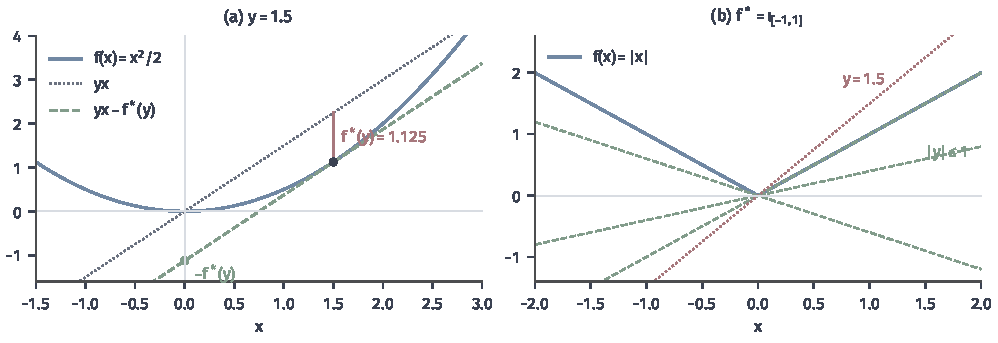
\includegraphics[width=169mm]{figures/03-optimization-evolution-and-signals/01-optimization/matplotlib/c5-conjugate/figure.pdf}
  \caption{共轭是最高仿射下界的截距。(a) $f(x)=x^2/2$，灰色点线为$yx$（$y=1.5$），绿色虚线为把它下移$f^*(y)=1.125$后的切线，红色线段是两者在$x=y$处的竖直间隔，绿点为截距$-f^*(y)$。(b) $f(x)=|x|$，绿色虚线为斜率$-0.6,0.4,1$的支撑直线，都经过原点；红色点线斜率为$1.5$，在$x>0$处超过$f$，不能平移成下界，故$f^*=\iota_{[-1,1]}$。}
  \label{fig:opt-con-conjugate}
\end{figure*}

共轭可以直接写出对偶函数。对线性等式约束问题$\min f(\bm x)$、$\bm A\bm x=\bm b$，
\[
  \begin{aligned}
    q(\bm\nu)&=\inf_{\bm x}\{f(\bm x)+\bm\nu^\top(\bm A\bm x-\bm b)\}
    =-\sup_{\bm x}\{\langle-\bm A^\top\bm\nu,\bm x\rangle-f(\bm x)\}-\bm b^\top\bm\nu\\
    &=-f^*(-\bm A^\top\bm\nu)-\bm b^\top\bm\nu.
  \end{aligned}
\]
等式二次例中$\bm Q=\operatorname{diag}(1,4)$、$\bm A=(1,1)$、$b=1$，代入$f^*(\bm y)=\frac12\bm y^\top\bm Q^{-1}\bm y$得$q(\nu)=-\frac12\nu^2(1+\frac14)-\nu=-\frac58\nu^2-\nu$，与直接计算一致。

\paragraph{从投影到分离超平面}
共轭用仿射函数从下方描述函数；对集合，相应的工具是用超平面把一点与集合分开。第~\ref{chap:opt-nonsmooth}章把投影建立为指示函数的邻近映射：对非空闭凸集$C$和任意$\bm z$，投影$\bm p=\Pi_C(\bm z)$存在唯一，并满足
\begin{equation}
\label{eq:opt-con-projection-vi}
  \langle\bm z-\bm p,\bm x-\bm p\rangle\leq0\qquad\text{对所有}\ \bm x\in C.
\end{equation}
这里只用这一不等式，不重复存在性的证明。

\begin{theorem}[点与闭凸集的严格分离]
\label{thm:opt-con-separation}
设$C\subseteq\mathbb R^d$非空闭凸，$\bm z\notin C$。则存在$\bm a\neq\bm0$与$\beta\in\mathbb R$，使$\langle\bm a,\bm x\rangle\leq\beta<\langle\bm a,\bm z\rangle$对所有$\bm x\in C$成立。
\end{theorem}

\begin{proof}
令$\bm p=\Pi_C(\bm z)$、$\bm a=\bm z-\bm p$、$\beta=\langle\bm a,\bm p\rangle$。$\bm z\notin C$而$\bm p\in C$，故$\bm a\neq\bm0$。式~\eqref{eq:opt-con-projection-vi}即$\langle\bm a,\bm x\rangle\leq\beta$；又$\langle\bm a,\bm z\rangle=\beta+\lVert\bm a\rVert_2^2>\beta$。
\end{proof}

超平面$\{\bm x:\langle\bm a,\bm x\rangle=\beta\}$称为\term{分离超平面}（separating hyperplane），它的法向量就是外点到投影点的连线方向。证明的关键是“闭”：若$C$不闭，外点可能落在$C$的闭包上，最近点不存在。

\paragraph{闭凸函数等于全体仿射下界的上确界}
把分离用在函数的上图$\operatorname{epi}f=\{(\bm x,r):r\geq f(\bm x)\}$上：$f$凸等价于上图凸，$f$下半连续等价于上图闭。于是对上图之外的点$(\bm x,r)$（即$r<f(\bm x)$），存在一个超平面把它与上图分开；只要这个超平面不是竖直的，它就是$f$的一个仿射下界，在$\bm x$处的值超过$r$。收集全部仿射下界，就能从下方把$f$完整地恢复出来。用共轭的语言，全体仿射下界的上确界是双共轭$f^{**}(\bm x)=\sup_{\bm y}\{\langle\bm y,\bm x\rangle-f^*(\bm y)\}$，而由Fenchel--Young不等式总有$f^{**}\leq f$。

\begin{theorem}[有限维Fenchel--Moreau定理]
\label{thm:opt-con-fenchel-moreau}
设$f:\mathbb R^d\to\mathbb R\cup\{+\infty\}$适当、下半连续且凸，则$f^{**}=f$。
\end{theorem}

\begin{proof}[证明（补充阅读）]
\emph{存在一个仿射下界。}上图非空闭凸。任取$\bm x_0\in\operatorname{dom}f$和$r_0<f(\bm x_0)$，对点$(\bm x_0,r_0)$与上图应用定理~\ref{thm:opt-con-separation}，得到$(\bm a,b)\neq\bm0$和$\beta$，使$\langle\bm a,\bm x\rangle+br\geq\beta>\langle\bm a,\bm x_0\rangle+br_0$对所有$(\bm x,r)\in\operatorname{epi}f$成立（必要时把分离向量取负）。上图沿$r$向上无界，所以$b\geq0$；若$b=0$，代入$(\bm x_0,f(\bm x_0))$得$\langle\bm a,\bm x_0\rangle\geq\beta>\langle\bm a,\bm x_0\rangle$，矛盾。故$b>0$，两边除以$b$得到仿射下界$\ell_0(\bm x)=\langle\bm y_0,\bm x\rangle-\beta_0\leq f(\bm x)$。

\emph{在每一点逼近$f$。}任取$\bm x$和$r<f(\bm x)$（$f(\bm x)=+\infty$时$r$可取任意实数），再次分离$(\bm x,r)$与上图，得到$(\bm a,b)$、$\beta$。若$b>0$，同上得到仿射下界$\ell$且$\ell(\bm x)>r$。若$b=0$，即$\langle\bm a,\bm x'\rangle\geq\beta>\langle\bm a,\bm x\rangle$对所有$\bm x'\in\operatorname{dom}f$成立；把它与$\varepsilon(r'-\ell_0(\bm x'))\geq0$（$(\bm x',r')\in\operatorname{epi}f$）相加，得到竖直系数为$\varepsilon>0$的不等式$\langle\bm a-\varepsilon\bm y_0,\bm x'\rangle+\varepsilon r'\geq\beta-\varepsilon\beta_0$。由于原来在$(\bm x,r)$处有严格间隙，$\varepsilon$取得足够小时它在$(\bm x,r)$处仍严格反向，于是又回到$b>0$的情形。两种情形都给出仿射下界$\ell(\bm x')=\langle\bm y,\bm x'\rangle-\beta'$满足$\ell(\bm x)>r$。由$\ell\leq f$得$f^*(\bm y)\leq\beta'$，所以$f^{**}(\bm x)\geq\langle\bm y,\bm x\rangle-f^*(\bm y)\geq\ell(\bm x)>r$。令$r\uparrow f(\bm x)$（或$r\to+\infty$）得$f^{**}(\bm x)\geq f(\bm x)$，与$f^{**}\leq f$合起来即得结论。
\end{proof}

闭性不能省略。$f=\iota_{(0,1)}$的共轭为$f^*(y)=\max\{0,y\}$，双共轭却是$\iota_{[0,1]}$，在两个端点补上了零值：仿射下界分辨不出开区间与它的闭包。还应注意，$f^{**}=f$说的是函数能由仿射下界重建，并没有说某个具体约束问题的对偶间隙为零；后者涉及约束与目标在同一个扰动集合上的联合结构，需要下一小节的条件。

\subsection{强对偶与乘子的存在}
\label{sec:opt-con-strong-duality}

当$d^\star=f^\star$时称\term{强对偶}（strong duality）成立。线性规划在原问题可行且有有限最优值时总有强对偶，第~\ref{chap:opt-linear-programming}章用单纯形的终止基证明了这一点。一般凸问题需要额外条件。图~\ref{fig:opt-con-dual-envelope}已经暗示了需要什么：对偶问题寻找的是在$u=0$处支撑“可达区域”的直线，只要这个区域在$u=0$附近有足够的“厚度”，非竖直的支撑直线就存在。

\paragraph{扰动值函数与Slater条件}
为了讨论“厚度”，把约束右端放松为$u$，定义扰动值函数$p(\bm u)=\inf\{f(\bm x):g_i(\bm x)\leq u_i\}$，并令$A=\{(\bm u,t):\text{存在}\ \bm x\ \text{使}\ g(\bm x)\leq\bm u,\ f(\bm x)\leq t\}$。$A$是$p$的上图（相差边界），$f$与$g_i$凸时$A$凸。对偶函数就是用斜率$-\bm\lambda$的超平面从下方支撑$A$时在$\bm u=\bm0$处的截距：$q(\bm\lambda)=\inf_{(\bm u,t)\in A}(t+\bm\lambda^\top\bm u)$。强对偶与对偶最优乘子的存在，等价于$A$在点$(\bm0,f^\star)$处有一个非竖直的支撑超平面。竖直的支撑超平面对应“$\bm u=\bm0$处于可达区域的边缘”，下面的条件正是排除这种情形。

第~\ref{chap:opt-nonsmooth}章在讨论次微分求和规则时解释过\term{相对内部}（relative interior）：集合可能落在一个低维仿射子空间里，此时它在整个$\mathbb R^d$中没有内点，但在自己的\term{仿射包}（affine hull）内仍可以有内点。下面的一般条件用相对内部表述，使低维定义域也能适用。

\begin{definition}[Slater条件]
\label{def:opt-con-slater}
设$f,g_i$是凸函数，$h_j$是仿射函数，$D=\operatorname{dom}f\cap\bigcap_i\operatorname{dom}g_i$为共同有效定义域。若存在$\bar{\bm x}\in\operatorname{ri}D$，使$g_i(\bar{\bm x})<0$对所有$i$成立且$h_j(\bar{\bm x})=0$对所有$j$成立，就说问题满足\term{Slater条件}（Slater's condition），$\bar{\bm x}$称为Slater点。
\end{definition}

Slater点要求不等式严格成立，留出余量；等式约束只要求满足，因为仿射等式不能“严格”成立；相对内部保证这个余量不是在定义域边缘上取得的。

\begin{theorem}[Slater条件下的强对偶]
\label{thm:opt-con-slater}
设问题~\eqref{eq:opt-con-problem}满足Slater条件，且$f^\star$有限。则$d^\star=f^\star$，并且对偶问题的最优值被某个$(\bm\lambda^\star,\bm\nu^\star)$达到。
\end{theorem}

\begin{proof}[仅含不等式且定义域为$\mathbb R^d$时的证明]
设$f,g_i$在$\mathbb R^d$上取有限值且凸，没有等式约束，Slater点$\bar{\bm x}$满足$g(\bar{\bm x})<\bm0$。

\emph{第一步：$(\bm0,f^\star-1/k)$不在$A$的闭包中。}若它属于闭包，存在$\bm x_n$使$g(\bm x_n)\leq\bm u_n\to\bm0$、$f(\bm x_n)\leq t_n\to f^\star-1/k$。对$\theta\in(0,1)$令$\bm x_n'=(1-\theta)\bm x_n+\theta\bar{\bm x}$，凸性给出$g(\bm x_n')\leq(1-\theta)\bm u_n+\theta g(\bar{\bm x})$与$f(\bm x_n')\leq(1-\theta)t_n+\theta f(\bar{\bm x})$。先取$\theta$足够小，使$(1-\theta)(f^\star-1/k)+\theta f(\bar{\bm x})<f^\star$；再取$n$足够大，使$g(\bm x_n')<\bm0$且$f(\bm x_n')<f^\star$。这是一个目标值低于$f^\star$的可行点，矛盾。

\emph{第二步：取分离方向的极限。}$A$的闭包是闭凸集。对每个$k$，定理~\ref{thm:opt-con-separation}给出单位向量$(\bm\lambda_k,\lambda_{0,k})$，使$\bm\lambda_k^\top\bm u+\lambda_{0,k}t>\bm\lambda_k^\top\bm0+\lambda_{0,k}(f^\star-1/k)$对$A$中全部点成立（已把分离向量取为指向$A$的一侧）。单位球紧，取收敛子列，极限$(\bm\lambda,\lambda_0)$仍是单位向量，并满足$\bm\lambda^\top\bm u+\lambda_0t\geq\lambda_0f^\star$对所有$(\bm u,t)\in A$成立。

\emph{第三步：法向量非竖直。}$A$中的点可以把$\bm u$的任一分量或$t$任意增大，所以$\bm\lambda\geq\bm0$、$\lambda_0\geq0$。若$\lambda_0=0$，则$\bm\lambda\neq\bm0$且$\bm\lambda^\top\bm u\geq0$对$A$中全部点成立；取$(\bm u,t)=(g(\bar{\bm x}),f(\bar{\bm x}))$，得$\bm\lambda^\top g(\bar{\bm x})\geq0$，但$\bm\lambda\geq\bm0$非零而$g(\bar{\bm x})<\bm0$，左端严格为负，矛盾。故$\lambda_0>0$。令$\bm\lambda^\star=\bm\lambda/\lambda_0\geq\bm0$，对任意$\bm x$取$(\bm u,t)=(g(\bm x),f(\bm x))$，得$f(\bm x)+\bm\lambda^{\star\top}g(\bm x)\geq f^\star$，即$q(\bm\lambda^\star)\geq f^\star$。结合弱对偶，$q(\bm\lambda^\star)=d^\star=f^\star$。
\end{proof}

一般情形（共同定义域的相对内部、加入仿射等式）的证明沿同一思路，但需要相对内部上的分离定理，可参考\scite{rockafellar1970convex}与\scite{math-boyd2004convex}。使用定理时要逐项核对：目标与不等式约束凸、等式约束仿射、Slater点在共同定义域的相对内部、最优值有限。定理保证零间隙和对偶最优乘子存在，却不保证原问题的最优点存在：$\min e^{-x}$、约束$-x\leq0$有Slater点$x=1$，$f^\star=0$，但没有点达到它。

图~\ref{fig:opt-con-slater}对比Slater条件成立与不成立的两种情形。左图仍是$\min x^2$、$1-x\leq u$，$p(u)=((1-u)_+)^2$在$u=0$附近两侧都有定义，斜率为$-\lambda^\star=-2$的直线在$u=0$处支撑它。右图是$\min x$、$x^2\leq u$：$u<0$时不可行，$p(u)=-\sqrt u$只在$u\geq0$上有定义，在$u=0$处切线竖直。此时Slater条件不成立（$x^2<0$无解），$q(\lambda)=\inf_x\{x+\lambda x^2\}=-1/(4\lambda)$随$\lambda\to\infty$趋于$0=f^\star$，间隙为零，但上确界不被任何有限乘子达到。这与第~\ref{sec:opt-con-optimality}节中$x^2\leq0$没有KKT乘子是同一现象的两个侧面。

\begin{figure*}[!htbp]
  \centering
  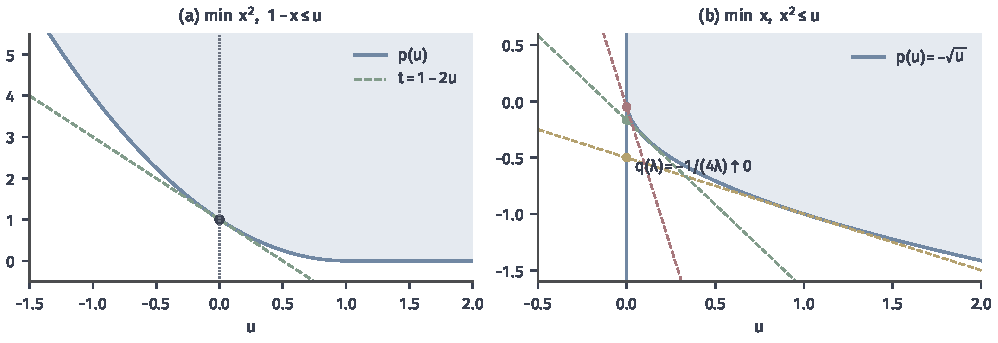
\includegraphics[width=169mm]{figures/03-optimization-evolution-and-signals/01-optimization/matplotlib/c5-slater/figure.pdf}
  \caption{扰动值函数$p(u)$与支撑直线。浅蓝区域为$p$的上图。(a) $\min x^2$、$1-x\leq u$：$p(u)=((1-u)_+)^2$，Slater点存在，绿色虚线$t=1-2u$在黑点$(0,1)$处支撑上图，斜率给出乘子$\lambda^\star=2$。(b) $\min x$、$x^2\leq u$：$u<0$不可行，$p(u)=-\sqrt u$在$u=0$处竖直；三条虚线是$\lambda=0.5,1.5,5$时的支撑直线，截距$q(\lambda)=-1/(4\lambda)$逐渐升向$0$，但没有有限斜率能达到。}
  \label{fig:opt-con-slater}
\end{figure*}

\paragraph{缺少条件时的反例}
线性规划的强对偶不能无条件推广。凸但不满足Slater条件的问题可以有正间隙：在定义域$x_2>0$上最小化$e^{-x_1}$，约束$x_1^2/x_2\leq0$。约束迫使$x_1=0$，故$f^\star=1$。而$\mathcal L=e^{-x_1}+\lambda x_1^2/x_2$，取$x_1=s$、$x_2=s^3$并令$s\to\infty$，得$\mathcal L\to0$，又$\mathcal L>0$，所以对每个$\lambda\geq0$都有$q(\lambda)=0$，$d^\star=0<1=f^\star$。约束函数$x_1^2/x_2$在$x_2>0$上凸，但它不可能严格小于零，Slater条件失败。非凸问题则可能有无穷大的间隙，如上一小节的$\min-x^2$，$x\in[-1,1]$。

\paragraph{KKT、零间隙与原始—对偶最优对}
下面的定理把第~\ref{sec:opt-con-optimality}节的候选检验与本节的界联系起来。

\begin{theorem}[零间隙与KKT条件]
\label{thm:opt-con-zero-gap-kkt}
(1) 若$\bm x^\star$可行、$\bm\lambda^\star\geq\bm0$且$f(\bm x^\star)=q(\bm\lambda^\star,\bm\nu^\star)$，则$\bm x^\star$是原问题的最优点，$(\bm\lambda^\star,\bm\nu^\star)$是对偶最优点，互补松弛成立，并且$\bm x^\star$是$\mathcal L(\cdot,\bm\lambda^\star,\bm\nu^\star)$的全局最小点；若各函数可微，则KKT条件成立。(2) 若原问题凸（$f,g_i$可微凸，$h_j$仿射）且$(\bm x^\star,\bm\lambda^\star,\bm\nu^\star)$满足KKT条件，则$f(\bm x^\star)=q(\bm\lambda^\star,\bm\nu^\star)$，两侧都最优。
\end{theorem}

\begin{proof}
(1) 由弱对偶，$f(\bm x^\star)=q(\bm\lambda^\star,\bm\nu^\star)\leq d^\star\leq f^\star\leq f(\bm x^\star)$，各处取等，两侧最优。又$q(\bm\lambda^\star,\bm\nu^\star)\leq\mathcal L(\bm x^\star,\bm\lambda^\star,\bm\nu^\star)=f(\bm x^\star)+\sum_i\lambda_i^\star g_i(\bm x^\star)\leq f(\bm x^\star)$，两端相等迫使$\sum_i\lambda_i^\star g_i(\bm x^\star)=0$；每一项非正，故逐项为零。同一串等式也说明$\mathcal L(\bm x^\star,\cdot)$达到下确界$q$，即$\bm x^\star$最小化$\mathcal L(\cdot,\bm\lambda^\star,\bm\nu^\star)$；可微时梯度为零，即驻点性。(2) 定理~\ref{thm:opt-con-kkt-sufficient}的证明已说明$\bm x^\star$最小化凸函数$\mathcal L(\cdot,\bm\lambda^\star,\bm\nu^\star)$，于是$q(\bm\lambda^\star,\bm\nu^\star)=\mathcal L(\bm x^\star,\bm\lambda^\star,\bm\nu^\star)=f(\bm x^\star)$。
\end{proof}

这条定理说明，在凸问题中“找到KKT点”与“找到零间隙的原始—对偶对”是同一件事。实际检验候选时仍要把几个问题分开：Slater条件或LICQ回答乘子是否存在；凸性回答KKT候选是否全局最优；原始最优点是否存在需要另外的紧性或强制性论证；而对于手中已有的有限精度候选，最可靠的是式~\eqref{eq:opt-con-gap-certificate}的上下界，它只依赖弱对偶。“强对偶成立”本身只是关于两个最优值的陈述，并不意味着已经找到了原始最优点。

\section{参数敏感性}
\label{sec:opt-con-sensitivity}

章首问过：预算从$2$增加到$2.1$，最优值会下降多少？这类问题改变的是问题数据，而不是求解过程。本节固定建模形式，让约束右端或其他参数变化，分别研究两个输出：最优值怎样变，最优解怎样变。二者需要的条件不同：最优值的变化可以由对偶乘子给出可靠的单侧界，即使值函数不可微；最优解的变化则要求KKT方程组在参数附近有可微的解分支。

\subsection{最优值的变化}
\label{sec:opt-con-value-sensitivity}

\paragraph{乘子给出的支撑界}
把约束的右端放松为参数，考虑
\begin{equation}
\label{eq:opt-con-perturbed}
  p(\bm u,\bm v)=\inf\{f(\bm x):g_i(\bm x)\leq u_i,\ h_j(\bm x)=v_j\},
\end{equation}
不可行时记$p=+\infty$。$\bm u_i>0$表示放宽第$i$条不等式，$u_i<0$表示收紧。上一节的扰动值函数就是这个函数在$\bm v=\bm0$时的情形。

\begin{theorem}[最优值的全局支撑界]
\label{thm:opt-con-global-sensitivity}
设未扰动问题的强对偶成立，且对偶最优值被$(\bm\lambda^\star,\bm\nu^\star)$达到。则对所有$(\bm u,\bm v)$，
\begin{equation}
\label{eq:opt-con-sensitivity-bound}
  p(\bm u,\bm v)\geq p(\bm0,\bm0)-\langle\bm\lambda^\star,\bm u\rangle-\langle\bm\nu^\star,\bm v\rangle.
\end{equation}
\end{theorem}

\begin{proof}
若扰动问题不可行，左端为$+\infty$，结论成立。否则任取扰动问题的可行点$\bm x$。由$\bm\lambda^\star\geq\bm0$、$g_i(\bm x)\leq u_i$、$h_j(\bm x)=v_j$，
\[
  p(\bm0,\bm0)=q(\bm\lambda^\star,\bm\nu^\star)\leq\mathcal L(\bm x,\bm\lambda^\star,\bm\nu^\star)\leq f(\bm x)+\langle\bm\lambda^\star,\bm u\rangle+\langle\bm\nu^\star,\bm v\rangle.
\]
移项后对可行$\bm x$取下确界即得。
\end{proof}

这个界只用到强对偶与对偶达到，不要求原问题凸，也不要求$p$可微；它对任意大小的扰动都成立，只是方向是单侧的。读法如下：收紧第$i$条约束（$u_i<0$）时，最优值至少增加$\lambda_i^\star|u_i|$，所以大乘子提示这条约束一收紧代价就很高；放宽它（$u_i>0$）时，最优值至多下降$\lambda_i^\star u_i$，但实际下降可能更少。这与第~\ref{chap:opt-linear-programming}章固定最优基时对偶变量作为资源价格的解释一致；线性规划中只要最优基不变，界就取等号，换基后才出现偏差。

回到章首：预算分配例在$\tau=2$时乘子$\lambda_1^\star=1/2$，最优值$V(2)=1/4$。预算约束写成$x_1+x_2-2\leq u$，$u=\tau-2$。界~\eqref{eq:opt-con-sensitivity-bound}给出$V(\tau)\geq\frac14-\frac12(\tau-2)$。直接计算可知$1\leq\tau\leq3$时$V(\tau)=(3-\tau)^2/4$，于是$V(2.2)=0.16\geq0.15$，$V(1.8)=0.36\geq0.35$。预算增加$0.1$时，最优值至多下降$0.05$，实际下降$0.25-0.2025=0.0475$。

\paragraph{乘子何时是导数}
如果$p$恰好在$(\bm0,\bm0)$处可微，界~\eqref{eq:opt-con-sensitivity-bound}立刻给出导数：函数$\varphi(\bm u,\bm v)=p(\bm u,\bm v)-p(\bm0,\bm0)+\langle\bm\lambda^\star,\bm u\rangle+\langle\bm\nu^\star,\bm v\rangle$非负且在原点为零，原点是它的最小点，可微时梯度为零，于是
\begin{equation}
\label{eq:opt-con-multiplier-derivative}
  \frac{\partial p}{\partial u_i}(\bm0,\bm0)=-\lambda_i^\star,\qquad
  \frac{\partial p}{\partial v_j}(\bm0,\bm0)=-\nu_j^\star.
\end{equation}
预算分配例中$V'(\tau)=-(3-\tau)/2=-\lambda_1^\star(\tau)$，在$\tau=2$处为$-1/2$。图~\ref{fig:opt-con-sensitivity}(a)画出$V(\tau)$和乘子曲线：红色点线是$\tau=2$处斜率为$-1/2$的支撑直线，整条曲线位于它的上方；$\tau\geq3$时预算不再限制解，乘子为零，$V$保持为零；$0<\tau<1$时第二个非负约束也活跃，$V(\tau)=((2-\tau)^2+1)/2$，乘子为$2-\tau$。三段在$\tau=1$与$\tau=3$处衔接时乘子连续，所以$V$仍然可微，只是二阶导数跳变。

可微性不能省略。考虑$\min-x$、约束$x\leq b$与$x\leq1$。当$b<1$时$V(b)=-b$，当$b>1$时$V(b)=-1$，即$V(b)=\max\{-b,-1\}$。在$b=1$处两条约束都活跃，驻点方程$-1+\lambda_1+\lambda_2=0$允许任意$\lambda_1\in[0,1]$、$\lambda_2=1-\lambda_1$，乘子不唯一。每个$\lambda_1$都给出一条斜率为$-\lambda_1$的支撑直线（图~\ref{fig:opt-con-sensitivity}(b)），所以无论向哪一侧改变$b$，界~\eqref{eq:opt-con-sensitivity-bound}都可靠；但$V$的左导数为$-1$、右导数为$0$，没有唯一的一阶变化率。多重乘子与值函数折点在这里同时出现：全部最优乘子的负值恰好组成$V$在折点处所有支撑斜率的集合$[-1,0]$。

\begin{figure*}[!htbp]
  \centering
  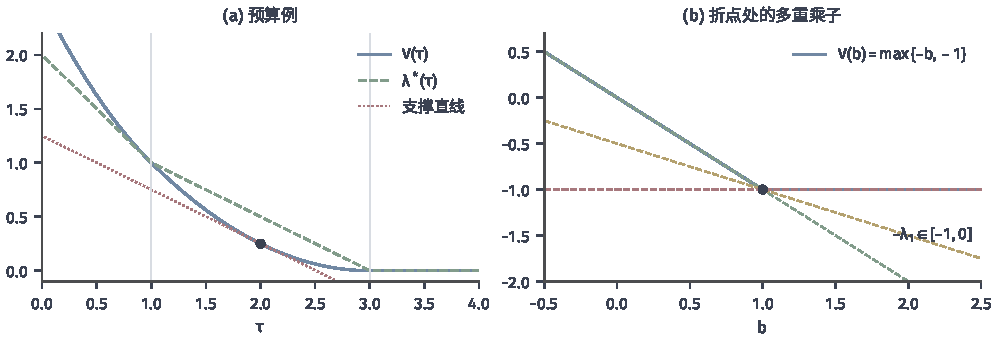
\includegraphics[width=169mm]{figures/03-optimization-evolution-and-signals/01-optimization/matplotlib/c5-sensitivity/figure.pdf}
  \caption{最优值随约束右端的变化。(a) 预算分配例：蓝线为最优值$V(\tau)$，绿色虚线为预算乘子$\lambda^\star(\tau)$，红色点线为$\tau=2$处斜率$-1/2$的支撑直线，灰色竖线标出活动集改变的$\tau=1,3$。(b) $\min-x$、$x\leq b$、$x\leq1$：$V(b)=\max\{-b,-1\}$在$b=1$处有折点，斜率$-1,-0.5,0$的三条虚线都是合法的支撑直线，对应不同的最优乘子。}
  \label{fig:opt-con-sensitivity}
\end{figure*}

\subsection{最优解的变化}
\label{sec:opt-con-solution-sensitivity}

最优值是一个数，最优解是一个向量，后者的变化需要更多结构。下面设目标与约束依赖参数$\theta$，且在$\theta_0$处有一个KKT点$(\bm x_0,\bm\lambda_0,\bm\nu_0)$。

\paragraph{固定活动集的KKT方程组}
设活动集为$I$，并且活跃约束的乘子都为正、未活跃约束严格满足（称为严格互补）。若参数变化后活动集保持为$I$，未活跃约束和它们的零乘子可以暂时忽略，解由下列方程组决定：
\[
  \bm F(\bm x,\bm\lambda_I,\bm\nu,\theta)=
  \begin{bmatrix}
    \nabla_{\bm x}\mathcal L(\bm x,\bm\lambda_I,\bm\nu,\theta)\\
    \bm g_I(\bm x,\theta)\\
    \bm h(\bm x,\theta)
  \end{bmatrix}=\bm0.
\]
记$\bm J$为活跃约束与等式约束的Jacobian（行为$\nabla g_i^\top$、$\nabla h_j^\top$），$\bm H=\nabla^2_{\bm x\bm x}\mathcal L$。方程组关于$(\bm x,\bm\lambda_I,\bm\nu)$的Jacobian是KKT矩阵
\begin{equation}
\label{eq:opt-con-kkt-matrix}
  \bm K=\begin{bmatrix}\bm H&\bm J^\top\\\bm J&\bm0\end{bmatrix}.
\end{equation}
若$\bm K$在$\theta_0$处可逆，隐函数定理（\BookChapterRef{chap:multivariate-calculus}{卷一“多元函数微分”章}）给出$\theta_0$附近唯一的连续可微解分支，导数由线性方程$\bm K\,\mathrm d(\bm x,\bm\lambda_I,\bm\nu)/\mathrm d\theta=-\partial\bm F/\partial\theta$确定。严格互补与连续性保证$\theta$足够接近$\theta_0$时活跃乘子仍为正、未活跃约束仍严格满足，因此这一分支确实是扰动问题的KKT点。

\begin{lemma}[KKT矩阵可逆的充分条件]
\label{lem:opt-con-kkt-matrix}
若$\bm J$行满秩（即LICQ），且$\bm H$在零空间$\ker\bm J$上正定（对所有非零$\bm d$，$\bm J\bm d=\bm0$蕴含$\bm d^\top\bm H\bm d>0$），则$\bm K$可逆。
\end{lemma}

\begin{proof}
设$\bm H\bm d+\bm J^\top\bm w=\bm0$、$\bm J\bm d=\bm0$。用$\bm d^\top$左乘第一式得$\bm d^\top\bm H\bm d=-(\bm J\bm d)^\top\bm w=0$，由零空间上的正定性得$\bm d=\bm0$；于是$\bm J^\top\bm w=\bm0$，行满秩给出$\bm w=\bm0$。
\end{proof}

预算分配例在$1<\tau<3$时活动集为$\{1\}$，$\bm H=\bm I$，$\bm J=(1,1)$。方程组为$\bm x-\bm c+\lambda(1,1)^\top=\bm0$、$x_1+x_2-\tau=0$，对$\tau$求导得$\bm x'+\lambda'(1,1)^\top=\bm0$、$x_1'+x_2'=1$，解出$\bm x'=(1/2,1/2)^\top$、$\lambda'=-1/2$，与显式解$\bm x^\star(\tau)=((\tau+1)/2,(\tau-1)/2)^\top$一致。

约束梯度独立本身并不保证$\bm K$可逆。最小化$\frac12x_2^2$、约束$x_2-\theta=0$，变量为$(x_1,x_2)$。约束梯度$(0,1)^\top$非零，LICQ成立；但$\bm H=\operatorname{diag}(0,1)$在$\ker\bm J=\{(t,0)^\top\}$上为零，$\bm K$奇异。对应地，解集$\{(x_1,\theta)^\top:x_1\in\mathbb R\}$是一条直线，“最优解对$\theta$的导数”根本没有确定的含义。

\paragraph{局部描述何时失效}
固定活动集的分析只在一个区间内有效。预算分配例在$\tau=1$与$\tau=3$处改变活动集：$\tau$跨过$3$时预算约束从带正乘子变为不起作用，$\bm x^\star(\tau)$的导数从$(1/2,1/2)^\top$跳到$\bm0$；跨过$1$时第二个非负约束开始活跃，导数跳到$(1,0)^\top$。在切换点，严格互补不成立（例如$\tau=3$时活跃约束的乘子为零），解仍然连续，但不可微。

局部驻点分支也不自动代表全局最优解。考虑$\min_x(x^2-1)^2+\theta x$。$\theta=0$时有两个全局最小点$\pm1$。驻点方程$4x(x^2-1)+\theta=0$在$(x,\theta)=(1,0)$处关于$x$的导数为$12x^2-4=8\neq0$，隐函数定理给出光滑分支$x(\theta)$，$x'(0)=-1/8$；在$-1$附近也有一条同样的分支。两条分支都是局部最小点，但$\theta>0$时$\theta x$项使$-1$附近的分支取更低的值，$\theta<0$时则相反。沿着$+1$分支计算导数是正确的，但这条分支在$\theta>0$时已不再是全局最优解；全局最优解在$\theta=0$处从一条分支跳到另一条，最优值的一阶近似为$-|\theta|$，出现折点。

最后，本节研究的是模型改变后\emph{精确}最优解和最优值的变化，与在同一问题上迭代截断、舍入或内层近似求解造成的误差是两回事。前者由KKT矩阵、活动集与乘子决定，后者由算法的收敛速度与停止规则决定。报告结果时应分开说明：数据扰动$\Delta\theta$通过导数或支撑界影响多少，计算误差又由残差或间隙证书控制到多少。二者都可能主导最终误差，却不能互相代替。

\section{二次规划与锥规划}
\label{sec:opt-con-quadratic-conic}

前三节的结论对一般的$f,g_i,h_j$成立。设计算法时，还要知道目标和约束具体是什么形状：同一个问题，写成二次规划、二阶锥规划还是半正定规划，决定了可以调用哪种子问题求解器、需要多少存储。本节按“目标与约束能写成什么结构”辨认三类常用模型，并说明哪些问题可以等价改写进来。这三类模型彼此包含：线性规划是二次规划的特例，凸二次规划可以写成二阶锥规划，二阶锥约束又可以写成半正定约束；它们不是互斥的分类，而是表达能力逐级增强、求解代价逐级增加的一组工具。为避免与最小二乘的数据矩阵$\bm A,\bm b$混淆，本节把线性约束写成$\bm E\bm x=\bm e$与$\bm G\bm x\leq\bm r$。

\subsection{二次规划}
\label{sec:opt-con-qp}

\paragraph{定义与凸性}
在线性约束下最小化平方误差，是最常见的约束问题之一。例如要求系数非负的最小二乘$\min\frac12\lVert\bm A\bm x-\bm b\rVert_2^2$、$\bm x\geq\bm0$，展开后目标是$\frac12\bm x^\top\bm A^\top\bm A\bm x-\bm b^\top\bm A\bm x+\text{常数}$。一般地，称
\begin{equation}
\label{eq:opt-con-qp}
  \min_{\bm x}\ \frac12\bm x^\top\bm P\bm x+\bm a^\top\bm x
  \quad\text{s.t.}\quad\bm E\bm x=\bm e,\quad\bm G\bm x\leq\bm r
\end{equation}
为\term{二次规划}（quadratic program），其中$\bm P$对称。目标的Hessian处处等于$\bm P$，所以目标凸当且仅当$\bm P\succeq\bm0$；$\bm P$有负特征值时，问题是非凸二次规划，一般可能有许多局部最小点，求全局最优通常是困难的。预算分配例是$\bm P=\bm I$的凸二次规划。最小二乘的线性方程解法见\BookChapterRef{chap:linear-equations-and-optimization}{卷一“线性方程与矩阵方程”章}，这里关心的是约束带来的新结构。

\paragraph{三种情形中的计算职责}
没有约束时，凸二次目标的最优条件是线性方程$\bm P\bm x=-\bm a$；它有解当且仅当$\bm a$在$\bm P$的值域中。只有等式约束时，KKT条件仍是线性方程组
\[
  \begin{bmatrix}\bm P&\bm E^\top\\\bm E&\bm0\end{bmatrix}
  \begin{bmatrix}\bm x\\\bm\nu\end{bmatrix}
  =\begin{bmatrix}-\bm a\\\bm e\end{bmatrix},
\]
其系数矩阵就是式~\eqref{eq:opt-con-kkt-matrix}的KKT矩阵；$\bm E$行满秩且$\bm P$在$\ker\bm E$上正定时，引理~\ref{lem:opt-con-kkt-matrix}保证它可逆，解唯一。等式二次例就是这种情形，一次线性求解便给出$(\bm x^\star,\nu^\star)$。

含不等式时困难在于不知道哪些约束活跃。若猜中最优点的活动集$I$，把$I$中的不等式当作等式，问题就退化为等式约束二次规划；解出后检查两件事：未列入$I$的约束是否满足，列入$I$的约束乘子是否非负。两项都通过，由凸问题的KKT充分性即得最优解；否则调整猜测，加入被违反的约束或删去乘子为负的约束。这就是\term{活动集法}（active-set method）的思路。预算分配例$\tau=2$时，先猜$I=\emptyset$得$\bm x=\bm c=(2,1)^\top$，违反预算；改猜$I=\{1\}$，解出$\bm x=(3/2,1/2)^\top$、$\lambda_1=1/2\geq0$，非负约束也满足，停止。活动集的组合数随约束数指数增长，最坏情形下活动集法可能尝试很多次；内点法（第~\ref{sec:opt-con-interior-point}节）则绕开了组合选择。

\paragraph{半正定但不正定时}
$\bm P\succeq\bm0$但奇异时，目标沿$\ker\bm P$的方向是线性的。若$\bm a$在某个可行的零空间方向上有负分量，目标无下界：无约束的$\min\frac12x_1^2+x_2$沿$x_2\to-\infty$无下界。若$\bm a$与这些方向正交，最优点不唯一：$\min\frac12x_1^2$的最优解集是整条$x_2$轴。加入约束可以改变这两种情形，例如再要求$x_2\geq0$，$\min\frac12x_1^2+x_2$的唯一解变为$\bm0$。所以检查二次规划时要分别核对：$\bm P$的惯性（凸性）、零空间方向上目标与约束的关系（有界性与唯一性），以及可行域是否非空。第~\ref{sec:opt-con-sqp}节的序列二次规划在每一步求解一个二次规划，那里同样要先做这些检查。

\subsection{二阶锥规划}
\label{sec:opt-con-socp}

\paragraph{二阶锥}
许多约束形如“某个仿射向量的欧氏范数不超过一个仿射函数”，例如鲁棒线性约束或带误差球的定位问题。把这种约束抽象出来，就是下面的集合。

\begin{definition}[二阶锥与二阶锥规划]
\label{def:opt-con-socp}
集合$K_k=\{(\bm u,t)\in\mathbb R^{k-1}\times\mathbb R:\lVert\bm u\rVert_2\leq t\}$称为\term{二阶锥}（second-order cone）。形如
\[
  \min_{\bm x}\ \bm a^\top\bm x\quad\text{s.t.}\quad\lVert\bm F_i\bm x+\bm f_i\rVert_2\leq\bm c_i^\top\bm x+d_i\ (i=1,\dots,K),\quad\bm E\bm x=\bm e
\]
的问题称为\term{二阶锥规划}（second-order cone program），每条约束即$(\bm F_i\bm x+\bm f_i,\bm c_i^\top\bm x+d_i)\in K_{k_i}$。
\end{definition}

二阶锥是凸锥：范数的三角不等式与正齐次性保证它对加法和非负倍数封闭。约束的右端$\bm c_i^\top\bm x+d_i$不必另外要求非负，因为左端非负，满足约束就已迫使右端非负。图~\ref{fig:opt-con-soc}画出$k=3$时的二阶锥，它的形状像一个冰淇淋筒：高度为$t$的水平截面是半径为$t$的圆盘。点$(\bm u,t)=((0.3,0.2)^\top,0.8)$满足$\lVert\bm u\rVert_2\approx0.361\leq0.8$，位于锥内。

\begin{figure}[!htbp]
  \centering
  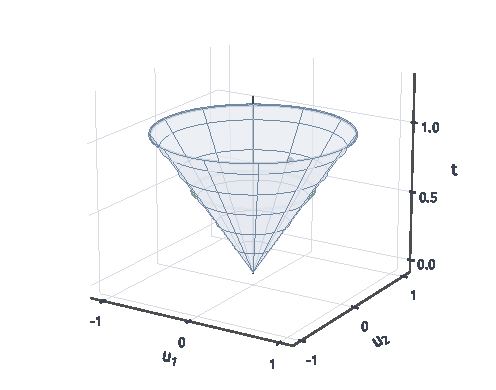
\includegraphics[width=84mm]{figures/03-optimization-evolution-and-signals/01-optimization/matplotlib/c5-soc/figure.pdf}
  \caption{$\mathbb R^3$中的二阶锥$\{(u_1,u_2,t):\sqrt{u_1^2+u_2^2}\leq t\}$，画出$0\leq t\leq1$的部分。蓝色圆为$t=1$的截面边界，绿色圆为$t=0.6$的截面边界，黑点$(0.3,0.2,0.8)$位于锥内。}
  \label{fig:opt-con-soc}
\end{figure}

\paragraph{把非线性不等式改写为锥成员条件}
改写的基本手段是引入上图变量。最小化范数$\lVert\bm A\bm x-\bm b\rVert_2$等价于在$\lVert\bm A\bm x-\bm b\rVert_2\leq t$下最小化$t$：任何可行$(\bm x,t)$都有$t\geq\lVert\bm A\bm x-\bm b\rVert_2$，最优时$t$恰取等号，所以两问题的最优值相同，最优$\bm x$也相同。平方范数需要多一步。对$s,t\geq0$，
\begin{equation}
\label{eq:opt-con-rotated-cone}
  \lVert\bm u\rVert_2^2\leq st\iff\left\lVert\begin{pmatrix}2\bm u\\s-t\end{pmatrix}\right\rVert_2\leq s+t,
\end{equation}
因为右式平方后为$4\lVert\bm u\rVert_2^2+(s-t)^2\leq(s+t)^2$，即$4\lVert\bm u\rVert_2^2\leq4st$；而右式本身已蕴含$s+t\geq|s-t|$，即$s,t\geq0$。

\paragraph{凸二次规划的锥形式}
设$\bm P\succeq\bm0$，取一个因子分解$\bm P=\bm F^\top\bm F$（如Cholesky分解或由谱分解得到）。目标$\frac12\bm x^\top\bm P\bm x+\bm a^\top\bm x=\frac12\lVert\bm F\bm x\rVert_2^2+\bm a^\top\bm x$。引入$t$，问题等价于
\[
  \min_{\bm x,t}\ t+\bm a^\top\bm x\quad\text{s.t.}\quad\left\lVert\begin{pmatrix}2\bm F\bm x\\2-t\end{pmatrix}\right\rVert_2\leq2+t,
\]
这里用式~\eqref{eq:opt-con-rotated-cone}取$\bm u=\bm F\bm x$、$s=2$，约束等价于$\frac12\lVert\bm F\bm x\rVert_2^2\leq t$。原问题的每个可行$\bm x$配上$t=\frac12\lVert\bm F\bm x\rVert_2^2$都可行且目标值不变；反过来，锥问题的任一可行$(\bm x,t)$都有$t\geq\frac12\lVert\bm F\bm x\rVert_2^2$，丢掉$t$后$\bm x$的原目标值不超过锥目标值。所以两问题最优值相等，最优$\bm x$相同，恢复时只需丢弃辅助变量。

这样的改写扩大了变量维数，还需要先对$\bm P$作分解。若$\bm P$稀疏而$\bm F$稠密，或$\bm P$只能通过矩阵向量积访问，保留二次结构直接求解往往更省；改写的好处是能把多种二次项和范数项统一交给锥规划求解器。改写也有边界：含平方项不等于凸。约束$\bm x^\top\bm Q\bm x\leq1$在$\bm Q$有负特征值时定义的是非凸集（如$x_1^2-x_2^2\leq1$是两条双曲线之间的区域），不能写成二阶锥约束；这类非凸二次约束要等到第~\ref{sec:opt-con-sdp-relaxation}节用松弛处理。

\subsection{半正定规划}
\label{sec:opt-con-sdp}

\paragraph{矩阵变量与迹内积}
有些约束天然落在矩阵上，例如协方差矩阵必须半正定、矩阵的最小特征值要尽量大。设$\mathbb S^k$为$k\times k$实对称矩阵组成的空间，在其上使用\term{Frobenius内积}（Frobenius inner product）$\langle\bm X,\bm Y\rangle=\operatorname{tr}(\bm X\bm Y)=\sum_{a,b}X_{a,b}Y_{a,b}$。线性目标与线性测量都写成这种内积。

\begin{definition}[半正定规划]
\label{def:opt-con-sdp}
给定$\bm C,\bm A_1,\dots,\bm A_m\in\mathbb S^k$与$\bm b\in\mathbb R^m$，问题
\[
  \min_{\bm X\in\mathbb S^k}\ \langle\bm C,\bm X\rangle\quad\text{s.t.}\quad\langle\bm A_i,\bm X\rangle=b_i\ (i=1,\dots,m),\quad\bm X\succeq\bm0
\]
称为（标准型）\term{半正定规划}（semidefinite program）。
\end{definition}

半正定锥$\{\bm X\succeq\bm0\}$是凸锥：若$\bm v^\top\bm X\bm v\geq0$、$\bm v^\top\bm Y\bm v\geq0$对所有$\bm v$成立，非负组合也满足。判断$\bm X\succeq\bm0$等价于全部特征值非负（\BookChapterRef{chap:linear-analysis}{卷一“谱和奇异值”章}），这与逐元素非负是两回事。$\begin{bmatrix}1&2\\2&1\end{bmatrix}$各元素为正，特征值却是$3$与$-1$；$\begin{bmatrix}1&-1\\-1&1\end{bmatrix}$有负元素，特征值$0$与$2$都非负。

图~\ref{fig:opt-con-psd-disk}把这一差别画出来。取迹为$1$的$2\times2$对称矩阵$\bm X=\begin{bmatrix}a&b\\b&1-a\end{bmatrix}$，它由两个数$(a,b)$决定。$\bm X\succeq\bm0$等价于对角元非负且行列式$a(1-a)-b^2\geq0$，即$(a-\frac12)^2+b^2\leq\frac14$：半正定的矩阵组成一个圆盘。逐元素非负要求$0\leq a\leq1$、$b\geq0$，是一条竖带的上半部分。圆盘的下半部分有负元素却半正定，竖带中圆盘以外的部分元素非负却不半正定。

\begin{figure}[!htbp]
  \centering
  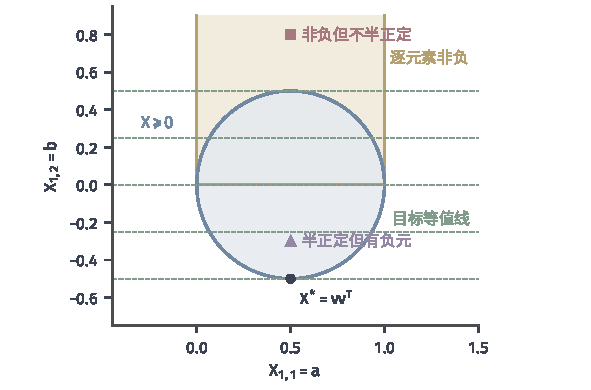
\includegraphics[width=100mm]{figures/03-optimization-evolution-and-signals/01-optimization/matplotlib/c5-psd-disk/figure.pdf}
  \caption{迹为$1$的$2\times2$对称矩阵$\begin{bmatrix}a&b\\b&1-a\end{bmatrix}$。蓝色圆盘为半正定矩阵$(a-\frac12)^2+b^2\leq\frac14$，黄色区域为逐元素非负的矩阵。红色方块$(0.5,0.8)$元素非负但不半正定，紫色三角$(0.5,-0.3)$半正定但有负元素。绿色虚线是目标$\langle\bm C,\bm X\rangle=2+2b$（$\bm C=\begin{bmatrix}2&1\\1&2\end{bmatrix}$）的等值线，最小值在圆盘最低点$\bm X^\star=\bm v\bm v^\top$处取得。}
  \label{fig:opt-con-psd-disk}
\end{figure}

\paragraph{Schur补}
半正定约束常用来表达非线性不等式，工具是Schur补。

\begin{lemma}[Schur补判别]
\label{lem:opt-con-schur}
设$\bm A\succ\bm0$，则$\begin{bmatrix}\bm A&\bm B\\\bm B^\top&\bm D\end{bmatrix}\succeq\bm0$当且仅当\term{Schur补}（Schur complement）$\bm D-\bm B^\top\bm A^{-1}\bm B\succeq\bm0$。
\end{lemma}

\begin{proof}
令$\bm T=\begin{bmatrix}\bm I&-\bm A^{-1}\bm B\\\bm0&\bm I\end{bmatrix}$，它可逆，且
\[
  \bm T^\top\begin{bmatrix}\bm A&\bm B\\\bm B^\top&\bm D\end{bmatrix}\bm T=\begin{bmatrix}\bm A&\bm0\\\bm0&\bm D-\bm B^\top\bm A^{-1}\bm B\end{bmatrix}.
\]
合同变换保持半正定性，块对角矩阵半正定当且仅当两块都半正定，而$\bm A\succ\bm0$已知。
\end{proof}

例如$\lVert\bm x\rVert_2^2\leq t$等价于$\begin{bmatrix}\bm I&\bm x\\\bm x^\top&t\end{bmatrix}\succeq\bm0$：这里$\bm A=\bm I$，Schur补为$t-\bm x^\top\bm x$。非线性的平方约束变成了对$(\bm x,t)$线性的矩阵不等式。引理要求左上块正定；左上块只半正定时，还需要“$\bm B$的列在$\bm A$的值域中”这一类附加条件，并把逆换成伪逆，不能直接套用上面的结论。

\paragraph{对偶锥与矩阵乘子}
半正定规划的对偶要用矩阵形式的乘子。对锥$K$，称$K^*=\{\bm Y:\langle\bm Y,\bm X\rangle\geq0\ \text{对所有}\ \bm X\in K\}$为它的\term{对偶锥}（dual cone）。非负象限的对偶锥仍是非负象限，这正是标量不等式乘子要求非负的原因。半正定锥也是自对偶的：若$\bm X,\bm Y\succeq\bm0$，则$\langle\bm Y,\bm X\rangle=\operatorname{tr}(\bm Y^{1/2}\bm X\bm Y^{1/2})\geq0$；反之若$\langle\bm Y,\bm X\rangle\geq0$对全部$\bm X\succeq\bm0$成立，取$\bm X=\bm v\bm v^\top$得$\bm v^\top\bm Y\bm v\geq0$。

对标准型半正定规划，把约束$\bm X\succeq\bm0$的乘子取为$\bm S\succeq\bm0$，Lagrange函数为$\langle\bm C,\bm X\rangle-\sum_iy_i(\langle\bm A_i,\bm X\rangle-b_i)-\langle\bm S,\bm X\rangle$，关于$\bm X$的下确界有限当且仅当$\bm C-\sum_iy_i\bm A_i=\bm S$。于是对偶问题为
\[
  \max_{\bm y}\ \bm b^\top\bm y\quad\text{s.t.}\quad\bm S=\bm C-\sum_iy_i\bm A_i\succeq\bm0.
\]
弱对偶可以直接核对：原始可行$\bm X$与对偶可行$\bm y$满足$\langle\bm C,\bm X\rangle-\bm b^\top\bm y=\langle\bm S,\bm X\rangle\geq0$。乘子的“非负”在这里是矩阵半正定$\bm S\succeq\bm0$，而不是逐元素非负。零间隙时$\langle\bm S,\bm X\rangle=0$，对两个半正定矩阵这等价于$\bm S\bm X=\bm0$，是矩阵形式的互补松弛。与标量情形一样，强对偶需要正则条件：若原问题有正定的可行矩阵$\bm X\succ\bm0$且最优值有限，则零间隙成立且对偶最优值达到\scite{math-boyd2004convex}。

\begin{example}[最小特征值的半正定规划]
\label{ex:opt-con-sdp-eigen}
取$\bm C=\begin{bmatrix}2&1\\1&2\end{bmatrix}$，最小化$\langle\bm C,\bm X\rangle$，约束$\operatorname{tr}\bm X=1$、$\bm X\succeq\bm0$。在图~\ref{fig:opt-con-psd-disk}的坐标中，目标为$2a+2b+2(1-a)=2+2b$，在圆盘最低点$(a,b)=(\frac12,-\frac12)$取最小值$1$，此时$\bm X^\star=\bm v\bm v^\top$，$\bm v=(1,-1)^\top/\sqrt2$。对偶问题为$\max y$、$\bm C-y\bm I\succeq\bm0$，即$y\leq\lambda_{\min}(\bm C)=1$，对偶最优值也是$1$。乘子矩阵$\bm S=\bm C-\bm I=\begin{bmatrix}1&1\\1&1\end{bmatrix}$满足$\bm S\bm v=\bm0$，故$\bm S\bm X^\star=\bm0$。原问题有正定可行点$\bm X=\frac12\bm I$，零间隙与上面的条件一致。
\end{example}

这个例子的最优解是秩一矩阵，对应$\bm C$最小特征值的特征向量。到此为止，问题本身给出的就是半正定规划，它已经是凸问题。怎样把一个非凸的二次问题放宽成半正定规划，再从松弛解中取回原问题的候选，是第~\ref{sec:opt-con-sdp-relaxation}节的另一项任务。

\section{在凸可行域内更新}
\label{sec:opt-con-feasible-updates}

从这一节起转向求解。最直接的想法是让每个迭代点都可行：只要可行域$C$是凸集，并且某个与$C$有关的小子问题容易求解，就可以在每一步把梯度信息转换成一个仍在$C$中的新点。本节对同一类问题——$f$在闭凸集$C$上光滑——比较三种做法。它们的区别只在于每步解哪一种子问题：投影梯度法解一个欧氏距离子问题，条件梯度法解一个线性子问题，镜像下降法把欧氏距离换成由参考函数确定的散度。

\subsection{投影梯度法}
\label{sec:opt-con-projected-gradient}

\paragraph{从梯度步到投影}
第~\ref{chap:opt-nonsmooth}章把投影建立为闭凸集指示函数的邻近映射：对非空闭凸集$C$，$\Pi_C(\bm z)=\argmin_{\bm x\in C}\lVert\bm x-\bm z\rVert_2$存在唯一，由式~\eqref{eq:opt-con-projection-vi}刻画，并且非扩张，即$\lVert\Pi_C(\bm z)-\Pi_C(\bm z')\rVert_2\leq\lVert\bm z-\bm z'\rVert_2$。\term{投影梯度法}（projected gradient method）把这一运算接在普通梯度步之后。在当前点$\bm x^{(t)}$处用线性模型加距离项近似目标，并只在$C$中最小化：
\[
  \bm x^{(t+1)}=\argmin_{\bm x\in C}\Bigl\{\langle\nabla f(\bm x^{(t)}),\bm x-\bm x^{(t)}\rangle+\frac1{2\eta}\lVert\bm x-\bm x^{(t)}\rVert_2^2\Bigr\}
  =\Pi_C\bigl(\bm x^{(t)}-\eta\nabla f(\bm x^{(t)})\bigr),
\]
第二个等号由配方得到。这正是第~\ref{chap:opt-nonsmooth}章邻近梯度法在非光滑项取$\iota_C$时的形式。

\begin{algorithm}[投影梯度法]
\label{alg:opt-con-projected-gradient}
\begin{algorithmic}[1]
\Require 可行初值$\bm x^{(0)}\in C$，步长$\eta>0$（已知$L$时取$\eta\leq1/L$），容差$\epsilon$
\Ensure 可行点$\bm x^{(t)}$
\For{$t=0,1,2,\dots$}
  \State 计算梯度$\nabla f(\bm x^{(t)})$，形成中心$\bm z=\bm x^{(t)}-\eta\nabla f(\bm x^{(t)})$
  \State 求投影$\bm x^{(t+1)}=\Pi_C(\bm z)$
  \If{$\lVert\bm x^{(t)}-\bm x^{(t+1)}\rVert_2/\eta\leq\epsilon$}
    \State 返回$\bm x^{(t+1)}$
  \EndIf
\EndFor
\end{algorithmic}
\end{algorithm}

每轮的代价是一次梯度计算加一次投影。$L$未知时可以回溯：把$\eta$减半直到$f(\bm x^{(t+1)})\leq f(\bm x^{(t)})+\langle\nabla f(\bm x^{(t)}),\bm x^{(t+1)}-\bm x^{(t)}\rangle+\frac1{2\eta}\lVert\bm x^{(t+1)}-\bm x^{(t)}\rVert_2^2$，每次试探都要重新投影。

\paragraph{具体集合上的投影}
投影的数学性质是一般的，计算却依赖集合。盒约束$C=\{\bm l\leq\bm x\leq\bm u\}$可以逐坐标截断：$\Pi_C(\bm z)_k=\min\{u_k,\max\{l_k,z_k\}\}$，代价$O(d)$；例如$[0,1]^2$上$\bm z=(1.5,-0.3)^\top$的投影是$(1,0)^\top$。欧氏球$\{\lVert\bm x\rVert_2\leq R\}$的投影是$\bm z\cdot\min\{1,R/\lVert\bm z\rVert_2\}$。概率单纯形$\Delta=\{\bm x\geq\bm0,\ \sum_kx_k=1\}$的坐标被总和约束耦合，不能逐坐标截断。对$\min\frac12\lVert\bm p-\bm z\rVert_2^2$、$\sum_kp_k=1$、$\bm p\geq\bm0$写KKT条件：$p_k-z_k+\nu-\mu_k=0$，$\mu_k\geq0$，$\mu_kp_k=0$。$p_k>0$时$\mu_k=0$、$p_k=z_k-\nu$；$p_k=0$时$z_k-\nu=-\mu_k\leq0$。两种情况合写为
\[
  p_k=\max\{z_k-\nu,0\},
\]
所有坐标共用一个阈值$\nu$，它由$\sum_k\max\{z_k-\nu,0\}=1$确定。左端关于$\nu$连续单调递减，把$\bm z$从大到小排序后逐个尝试正坐标的个数即可求出，代价$O(d\log d)$。例如$\bm z=(0.8,0.6,-0.1)^\top$：假设前两个坐标为正，$\nu=(0.8+0.6-1)/2=0.2$，检验$0.6-0.2>0$、$-0.1-0.2<0$，假设成立，投影为$(0.6,0.4,0)^\top$。一般凸集的投影本身可能是一个需要迭代求解的优化问题。

\paragraph{停止残差与收敛}
由式~\eqref{eq:opt-con-projection-vi}，$\bm x=\Pi_C(\bm x-\eta\nabla f(\bm x))$当且仅当$\langle\bm x-\eta\nabla f(\bm x)-\bm x,\bm y-\bm x\rangle\leq0$对所有$\bm y\in C$成立，即$\bm x$满足变分不等式~\eqref{eq:opt-con-vi}。所以投影梯度映射
\[
  \bm G_\eta(\bm x)=\frac{\bm x-\Pi_C(\bm x-\eta\nabla f(\bm x))}{\eta}
\]
为零恰好刻画一阶条件，算法~\ref{alg:opt-con-projected-gradient}用它的范数作停止量。它在无约束时退化为$\nabla f(\bm x)$。第~\ref{chap:opt-nonsmooth}章对邻近梯度法的分析在这里直接适用：$f$在$C$上凸且$L$光滑、最小点存在、$\eta\leq1/L$时，$f(\bm x^{(T)})-f^\star\leq\lVert\bm x^{(0)}-\bm x^\star\rVert_2^2/(2\eta T)$；若$f$还$\mu$强凸，到最小点的距离按$1-\eta\mu$的比率线性收缩。$f$非凸时，小的$\lVert\bm G_\eta\rVert_2$只说明接近一个满足一阶条件的点。

图~\ref{fig:opt-con-pg-fw}(a)在三角形$\{\bm x\geq\bm0,\ x_1+x_2\leq2\}$上最小化$f(\bm x)=\frac12((x_1-2.5)^2+4(x_2-1)^2)$，$L=4$。无约束最小点$(2.5,1)^\top$在三角形外，约束最优点$(1.3,0.7)^\top$在斜边上，预算乘子为$1.2$，$f^\star=0.9$。从$\bm0$出发取$\eta=1/4$：梯度为$(-2.5,-4)^\top$，梯度步到达$(0.625,1)^\top$，已在三角形内，投影不起作用；下一步的梯度步越过斜边，被投影拉回斜边，此后迭代沿斜边逼近最优点，依次为$(1.047,0.953)^\top$、$(1.205,0.795)^\top$、$(1.264,0.736)^\top$。目标是强凸的，图(b)中目标差按几何级数下降。

\paragraph{预条件必须匹配投影}
若用固定的正定矩阵$\bm M$作预条件，梯度步变为$\bm x-\eta\bm M\nabla f(\bm x)$，投影也必须换成在范数$\lVert\bm v\rVert_{\bm M^{-1}}^2=\bm v^\top\bm M^{-1}\bm v$下的最近点：
\[
  \bm x^{+}=\argmin_{\bm y\in C}\ \bigl\lVert\bm y-(\bm x-\eta\bm M\nabla f(\bm x))\bigr\rVert_{\bm M^{-1}}^2.
\]
这样，固定点条件中的$\bm M^{-1}\bm M$相互抵消，仍是原来的变分不等式。若仍用欧氏投影，固定点满足的是$\langle\bm M\nabla f(\bm x),\bm y-\bm x\rangle\geq0$，一般与原条件不同。等式二次例给出一个具体反例：取$\bm M=\operatorname{diag}(1,4)$，在约束直线上$\bm M\nabla f=(x_1,16x_2)^\top$，欧氏投影的固定点要求它与直线方向$(1,-1)^\top$正交，得到$x_1=16x_2$，即$(16/17,1/17)^\top$，而真正的最优点是$(4/5,1/5)^\top$。对角$\bm M$加盒约束时加权投影仍可逐坐标计算；对单纯形或一般耦合的$\bm M$，加权投影是一个新的子问题，代价不能按欧氏投影计算。

\paragraph{近似投影}
投影若由内层迭代求出，输出与真投影之差$\zeta_t$会带来两类后果。其一，输出可能略微不可行，必须单独检查约束残差，不能把“投影子问题的距离误差小”当作可行。其二，误差会沿迭代传播：投影非扩张，若精确的投影梯度映射在凸、$L$光滑且$\eta\leq2/L$时把距离收缩不增，则到最优点的距离满足$\delta_{t+1}\leq\delta_t+\zeta_t$，强凸时可改进为$\delta_{t+1}\leq(1-\eta\mu)\delta_t+\zeta_t$，误差最终停留在$\zeta/(\eta\mu)$量级。停止量$\lVert\bm G_\eta\rVert_2$里的误差被放大为$\zeta_t/\eta$，步长很小时尤其明显。投影的存在唯一与非扩张、具体集合上投影怎么算、外层迭代收敛多快，是三项不同的职责。

\subsection{条件梯度法}
\label{sec:opt-con-frank-wolfe}

\paragraph{用线性子问题代替投影}
对某些集合，求投影很贵，但在集合上最小化一个线性函数很便宜。例如在迹不超过$\tau$的半正定矩阵集合上，投影需要完整的特征分解，而最小化线性函数只需要一个极端特征向量。下面的方法利用这一点：把目标在当前点线性化，在$C$上求线性模型的最小点，再沿当前点与该点的连线移动一段。$C$紧时线性子问题总有解，新点是两个可行点的凸组合，自动可行。这就是\term{条件梯度法}（conditional gradient method），由Frank与Wolfe提出\scite{frank1956algorithm}，也称Frank--Wolfe法。

\begin{algorithm}[条件梯度法]
\label{alg:opt-con-frank-wolfe}
\begin{algorithmic}[1]
\Require 非空紧凸集$C$上的线性最小化程序，可行初值$\bm x^{(0)}\in C$，容差$\epsilon$
\Ensure 可行点$\bm x^{(t)}$及条件梯度间隙
\For{$t=0,1,2,\dots$}
  \State 计算梯度，解线性子问题$\bm s^{(t)}\in\argmin_{\bm s\in C}\langle\nabla f(\bm x^{(t)}),\bm s\rangle$
  \State 计算间隙$\gamma_t=\langle\nabla f(\bm x^{(t)}),\bm x^{(t)}-\bm s^{(t)}\rangle$；若$\gamma_t\leq\epsilon$，返回$\bm x^{(t)}$
  \State 取步长$\alpha_t=2/(t+2)$（或在线段上作一维线搜索），更新$\bm x^{(t+1)}=\bm x^{(t)}+\alpha_t(\bm s^{(t)}-\bm x^{(t)})$
\EndFor
\end{algorithmic}
\end{algorithm}

\paragraph{线性子问题的稀疏与低秩解}
线性函数在紧凸集上的最小值总能在极点处取到，所以线性子问题的解往往很“简单”。在单纯形上，它是梯度最小坐标对应的顶点$\bm e_k$；从一个顶点出发，$t$步以后迭代点至多是$t+1$个顶点的凸组合，至多有$t+1$个非零坐标。在$\{\bm S\succeq\bm0,\ \operatorname{tr}\bm S\leq\tau\}$上，记$\bm W=\nabla f(\bm X)$的最小特征值为$\lambda_{\min}$、对应单位特征向量为$\bm v$。对该集合中任意$\bm S$，用$\bm S$的谱分解$\bm S=\sum_k\sigma_k\bm u_k\bm u_k^\top$得$\langle\bm W,\bm S\rangle=\sum_k\sigma_k\bm u_k^\top\bm W\bm u_k\geq\lambda_{\min}\operatorname{tr}\bm S\geq\tau\min\{\lambda_{\min},0\}$，所以$\lambda_{\min}<0$时线性子问题的解是秩一矩阵$\tau\bm v\bm v^\top$，否则是$\bm0$。迭代$t$步后，矩阵的秩至多为$t$，求解过程只需存储这些秩一因子。

\paragraph{条件梯度间隙与收敛速度}
算法中的$\gamma_t$同时是一份证书。若$f$凸，由一阶支撑下界，对最优点$\bm x^\star$，
\[
  f(\bm x^{(t)})-f^\star\leq\langle\nabla f(\bm x^{(t)}),\bm x^{(t)}-\bm x^\star\rangle\leq\max_{\bm s\in C}\langle\nabla f(\bm x^{(t)}),\bm x^{(t)}-\bm s\rangle=\gamma_t,
\]
因此不知道$f^\star$也能确定目标差的上界；$\gamma_t=0$恰好是变分不等式~\eqref{eq:opt-con-vi}。

\begin{theorem}[条件梯度法的收敛速度]
\label{thm:opt-con-frank-wolfe}
设$C$非空紧凸，直径为$D=\max_{\bm x,\bm y\in C}\lVert\bm x-\bm y\rVert_2$，$f$在$C$的开邻域上凸且$L$光滑。取$\alpha_t=2/(t+2)$，则对$t\geq1$，$f(\bm x^{(t)})-f^\star\leq2LD^2/(t+2)$。
\end{theorem}

\begin{proof}
记$e_t=f(\bm x^{(t)})-f^\star$。由$L$光滑的二次上界，并利用$\lVert\bm s^{(t)}-\bm x^{(t)}\rVert_2\leq D$与上式$\langle\nabla f(\bm x^{(t)}),\bm s^{(t)}-\bm x^{(t)}\rangle=-\gamma_t\leq-e_t$，
\[
  e_{t+1}\leq e_t+\alpha_t\langle\nabla f(\bm x^{(t)}),\bm s^{(t)}-\bm x^{(t)}\rangle+\frac{L\alpha_t^2D^2}{2}\leq(1-\alpha_t)e_t+\frac{L\alpha_t^2D^2}{2}.
\]
$t=0$时$\alpha_0=1$，得$e_1\leq LD^2/2\leq2LD^2/3$。若$e_t\leq2LD^2/(t+2)$，代入$\alpha_t=2/(t+2)$，
\[
  e_{t+1}\leq\frac{t}{t+2}\cdot\frac{2LD^2}{t+2}+\frac{2LD^2}{(t+2)^2}=\frac{2LD^2(t+1)}{(t+2)^2}\leq\frac{2LD^2}{t+3},
\]
最后一步用了$(t+1)(t+3)\leq(t+2)^2$。归纳即得。
\end{proof}

图~\ref{fig:opt-con-pg-fw}对比同一问题上的两种方法。条件梯度法从$\bm0$出发，第一步的线性子问题选中顶点$(0,2)^\top$（梯度$(-2.5,-4)^\top$与该顶点内积最小），步长$\alpha_0=1$，直接跳到该顶点；此后线性子问题在顶点$(2,0)^\top$与$(0,2)^\top$之间交替，迭代点沿斜边来回振荡逼近最优点。最优点位于斜边内部而不在顶点上，这种“之”字形使目标差只按$O(1/t)$减小并伴随振荡：$100$步时目标差约为$7\times10^{-5}$，而投影梯度法$15$步内已达到$10^{-12}$。条件梯度间隙也在振荡，所以实际停止时常记录迄今最小的间隙。

\begin{figure*}[!htbp]
  \centering
  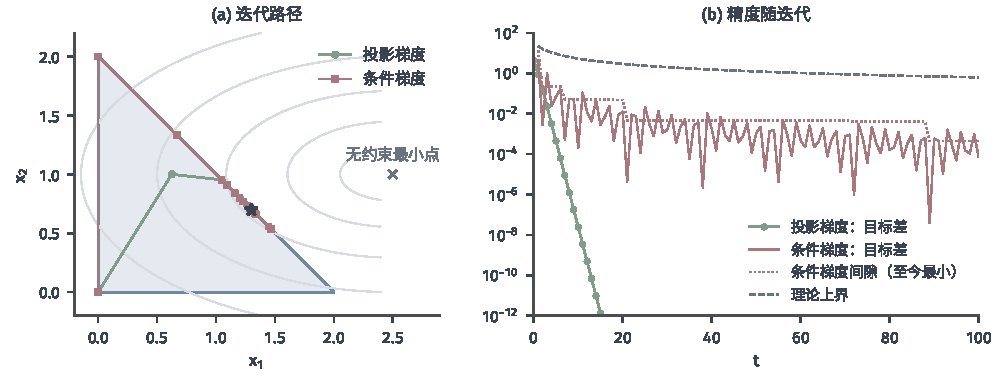
\includegraphics[width=169mm]{figures/03-optimization-evolution-and-signals/01-optimization/matplotlib/c5-pg-fw/figure.pdf}
  \caption{三角形$\{\bm x\geq\bm0,\ x_1+x_2\leq2\}$上最小化$\frac12((x_1-2.5)^2+4(x_2-1)^2)$，起点$\bm0$。(a) 灰色椭圆为等值线，五角星为最优点$(1.3,0.7)^\top$；绿色为投影梯度法（$\eta=1/4$），红色为条件梯度法（$\alpha_t=2/(t+2)$），后者在两个顶点之间交替选点，沿斜边振荡。(b) 对数纵轴上的目标差：投影梯度法线性收敛；条件梯度法的目标差振荡下降，红色点线为迄今最小的条件梯度间隙，灰色虚线为定理~\ref{thm:opt-con-frank-wolfe}的上界$2LD^2/(t+2)$，$L=4$，$D=2\sqrt2$。}
  \label{fig:opt-con-pg-fw}
\end{figure*}

两种方法应在同一精度口径下比较每轮成本。单纯形或盒约束上投影与线性子问题都很便宜，投影梯度法通常更快。迹约束的半正定集合上，投影需要$O(k^3)$的完整特征分解，而线性子问题只需一个极端特征向量，可用Lanczos类迭代以若干次矩阵向量积近似求得；条件梯度法因此常被用于低秩矩阵问题。代价是收敛较慢：最优点落在集合边界的面内部时，要获得高精度需要很多次迭代。

\subsection{镜像下降法}
\label{sec:opt-con-mirror-descent}

\paragraph{欧氏距离不总是合适的尺度}
在概率单纯形上，从$x_k=0.01$变到$0.02$与从$0.5$变到$0.51$的欧氏距离相同，但前者让这个坐标翻了一倍。投影梯度法用欧氏距离衡量步子，会在一步之内把小坐标截成零（图~\ref{fig:opt-con-mirror-simplex}中第三个坐标在第3步恰好变为零），而后续步骤只能从边界上重新开始。\term{镜像下降法}（mirror descent）把投影梯度法中的$\frac12\lVert\bm x-\bm x^{(t)}\rVert_2^2$换成一个更贴合集合几何的“距离”。

\begin{definition}[Bregman散度]
\label{def:opt-con-bregman}
设$\varphi$是在开凸集$\operatorname{int}\operatorname{dom}\varphi$上可微的严格凸函数，称
\[
  D_\varphi(\bm x,\bm y)=\varphi(\bm x)-\varphi(\bm y)-\langle\nabla\varphi(\bm y),\bm x-\bm y\rangle,\qquad\bm x\in\operatorname{dom}\varphi,\ \bm y\in\operatorname{int}\operatorname{dom}\varphi
\]
为$\varphi$生成的\term{Bregman散度}（Bregman divergence），$\varphi$称为参考函数。
\end{definition}

$D_\varphi(\bm x,\bm y)$是$\varphi$在$\bm x$处的值超出它在$\bm y$处切平面的部分；由严格凸性，它非负，且仅在$\bm x=\bm y$时为零。它一般不对称，也不满足三角不等式，所以不是度量。取$\varphi(\bm x)=\frac12\lVert\bm x\rVert_2^2$得$D_\varphi(\bm x,\bm y)=\frac12\lVert\bm x-\bm y\rVert_2^2$。取负熵$\varphi(\bm x)=\sum_kx_k\log x_k$（定义在$\bm x\geq\bm0$上，约定$0\log0=0$），对单纯形中的$\bm x$与正向量$\bm y\in\Delta$，$D_\varphi(\bm x,\bm y)=\sum_kx_k\log(x_k/y_k)$。例如$\bm x=(1/2,1/2)$、$\bm y=(1/4,3/4)$时$D_\varphi(\bm x,\bm y)=\frac12\log2+\frac12\log\frac23\approx0.144$，而$D_\varphi(\bm y,\bm x)=\frac14\log\frac12+\frac34\log\frac32\approx0.131$，两者不同。

\paragraph{镜像下降的更新}
把散度放进线性化子问题，镜像下降的一步为
\begin{equation}
\label{eq:opt-con-mirror-step}
  \bm x^{(t+1)}\in\argmin_{\bm x\in C\cap\operatorname{dom}\varphi}\Bigl\{\eta\langle\nabla f(\bm x^{(t)}),\bm x\rangle+D_\varphi(\bm x,\bm x^{(t)})\Bigr\}.
\end{equation}
它要求$\bm x^{(t)}$在$\varphi$的可微域内部，否则$D_\varphi(\cdot,\bm x^{(t)})$无定义；严格凸只保证子问题至多一个解，解的存在、以及解是否仍在可微域内部（下一步能否继续），要针对具体的$\varphi$和$C$另外核查。欧氏参考函数下，式~\eqref{eq:opt-con-mirror-step}就是投影梯度步。

在单纯形上取负熵，并从正权重出发。式~\eqref{eq:opt-con-mirror-step}的目标为$\sum_k(\eta g_kx_k+x_k\log(x_k/x_k^{(t)}))$，其中$\bm g=\nabla f(\bm x^{(t)})$（单纯形上$\sum_kx_k=\sum_kx_k^{(t)}$，散度中的线性项抵消）。对等式$\sum_kx_k=1$引入乘子$\nu$，令偏导为零：$\eta g_k+\log(x_k/x_k^{(t)})+1+\nu=0$，于是
\begin{equation}
\label{eq:opt-con-exponential-weights}
  x_k^{(t+1)}=\frac{x_k^{(t)}\exp(-\eta g_k)}{\sum_lx_l^{(t)}\exp(-\eta g_l)}.
\end{equation}
这是乘以指数因子再归一化的\emph{指数权重更新}。梯度有限时指数因子严格为正，正权重永远保持为正，非负约束从不活跃，所以忽略它们的拉格朗日计算是合法的；$\log$在边界处的无界导数自动把迭代挡在内部。

图~\ref{fig:opt-con-mirror-simplex}在单纯形上最小化$f(\bm x)=\frac12\lVert\bm x-\bm c\rVert_2^2$，$\bm c=(0.8,0.6,-0.1)^\top$，最优点是前面算过的投影$(0.6,0.4,0)^\top$，从$\bm x^{(0)}=(0.15,0.15,0.7)^\top$出发。镜像下降取$\eta=1$：$\bm g=\bm x^{(0)}-\bm c=(-0.65,-0.45,0.8)^\top$，未归一化的权重为$0.15e^{0.65}\approx0.2873$、$0.15e^{0.45}\approx0.2352$、$0.7e^{-0.8}\approx0.3145$，归一化得$\bm x^{(1)}\approx(0.343,0.281,0.376)^\top$。投影梯度取$\eta=0.5$：中心$\bm x^{(0)}-0.5\bm g=(0.475,0.375,0.3)^\top$，坐标和为$1.15$，共同阈值$0.05$，得$\bm x^{(1)}=(0.425,0.325,0.25)^\top$。两条路径都走向最优点，但投影梯度法在第3步把第三个坐标截为零后沿边界移动，镜像下降的第三个坐标始终为正，按指数速度趋于零。

\begin{figure*}[!htbp]
  \centering
  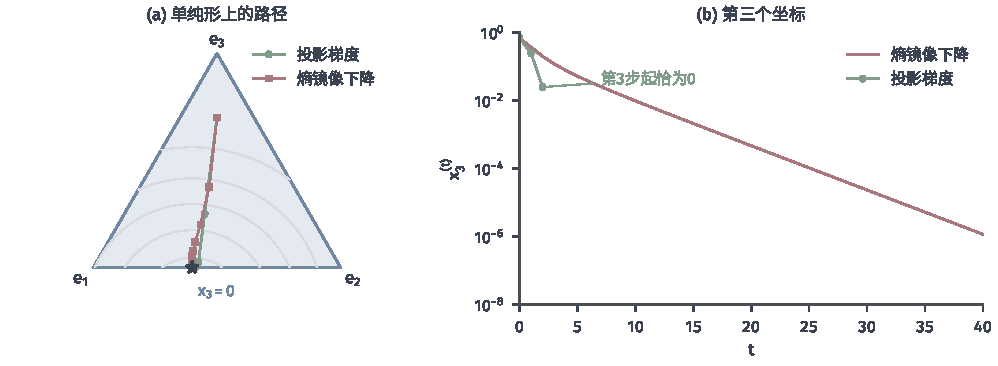
\includegraphics[width=169mm]{figures/03-optimization-evolution-and-signals/01-optimization/matplotlib/c5-mirror-simplex/figure.pdf}
  \caption{概率单纯形上最小化$\frac12\lVert\bm x-\bm c\rVert_2^2$，$\bm c=(0.8,0.6,-0.1)^\top$，起点$(0.15,0.15,0.7)^\top$。(a) 单纯形用重心坐标画成三角形，顶点$\bm e_k$对应第$k$个坐标为$1$，灰色曲线为目标等值线，五角星为最优点$(0.6,0.4,0)^\top$，位于$x_3=0$的边上。绿色为投影梯度法（$\eta=0.5$），红色为熵镜像下降（$\eta=1$）。(b) 第三个坐标随迭代的变化（对数纵轴）：投影梯度法在第3步起恰为零，镜像下降保持为正并几何下降。}
  \label{fig:opt-con-mirror-simplex}
\end{figure*}

参考函数的选择影响的不只是路径形状。对单纯形上的凸、梯度各分量有界（$\lVert\nabla f\rVert_\infty\leq G$）的问题，熵镜像下降的目标差界依赖$\sqrt{\log d}$，而欧氏投影的相应界依赖梯度的欧氏范数，可能大到$\sqrt dG$，维数高时前者显著更好\scite{beck2003mirror}。这里只建立有限维的优化机制。上面单纯形上的负熵散度就是离散分布之间的KL散度，它作为分布间散度的系统性质、相应的几何及统计解释，可参考\BookChapterRef{chap:information-theory-and-statistical-geometry}{卷四“概率分布的分析与优化”章}。

\section{惩罚法}
\label{sec:opt-con-penalty}

上一节要求每一步都可行，这需要投影或线性子问题容易求解。约束一旦是非线性的，或可行域的投影本身就是难题，这一要求便难以满足。惩罚法换一种思路：允许迭代点暂时违约，但给违约计价，把约束问题换成一个（或一列）无约束问题，交给第~\ref{chap:opt-smooth}章和第~\ref{chap:opt-nonsmooth}章的方法求解。计价方式决定了两种不同的目标：二次惩罚只在罚参数趋于无穷时逐步逼近可行，精确惩罚则在罚参数超过某个有限阈值后就保留原问题的解。下一节的乘子法会在惩罚之外再更新乘子。

\subsection{二次惩罚法}
\label{sec:opt-con-quadratic-penalty}

\paragraph{给违约的平方计价}
用约束残差构造违约度量$P(\bm x)=\sum_jh_j(\bm x)^2+\sum_i[g_i(\bm x)]_+^2$，其中$[t]_+=\max\{t,0\}$。$P\geq0$，且$P(\bm x)=0$当且仅当$\bm x$可行。对罚参数$\rho>0$，\term{二次惩罚法}（quadratic penalty method）求解
\begin{equation}
\label{eq:opt-con-quadratic-penalty}
  \min_{\bm x}\ Q_\rho(\bm x)=f(\bm x)+\frac\rho2P(\bm x).
\end{equation}
函数$[t]_+^2$连续可微，导数为$2[t]_+$，所以$f,g_i,h_j$连续可微时$Q_\rho$也连续可微，可以用梯度类方法求解；但$[t]_+^2$在$t=0$处二阶导数跳变，牛顿法在活动集变化处可能受影响。约束仿射时罚项是凸二次函数；约束非线性时，罚项一般不继承凸性，例如$h(x)=x^2-1$的平方$(x^2-1)^2$在$x=0$附近是凹的。

罚参数在原目标与违约之间取舍。对等式二次例，$Q_\rho=\frac12(x_1^2+4x_2^2)+\frac\rho2(x_1+x_2-1)^2$，令梯度为零：$x_1+\rho r=0$、$4x_2+\rho r=0$，其中$r=x_1+x_2-1$。于是$x_1=-\rho r$、$x_2=-\rho r/4$，代回$r$的定义得$r=-\frac54\rho r-1$，即
\[
  \bm x_\rho=\frac{(4\rho,\ \rho)^\top}{4+5\rho},\qquad
  h(\bm x_\rho)=-\frac{4}{4+5\rho}.
\]
任何有限的$\rho$都给出不可行的点，违约随$\rho$增大按$1/\rho$的速度减小，$\bm x_\rho$沿一条从原点出发的射线逼近$\bm x^\star=(4/5,1/5)^\top$（图~\ref{fig:opt-con-penalty-path}(a)）。顺带还能读出乘子：驻点方程与$\nabla f+\nu\nabla h=\bm0$对照，$\rho h(\bm x_\rho)=-4\rho/(4+5\rho)$扮演乘子的角色，并随$\rho\to\infty$趋于$\nu^\star=-4/5$。这一观察是下一节增广Lagrange法的出发点。

\begin{algorithm}[二次惩罚法]
\label{alg:opt-con-quadratic-penalty}
\begin{algorithmic}[1]
\Require 初值$\bm x^{(0)}$，初始罚参数$\rho_0>0$，放大因子$\beta>1$，内层容差序列$\epsilon_k\to0$，可行性容差$\epsilon_{\mathrm{feas}}$
\Ensure 近似可行的候选$\bm x_k$
\For{$k=0,1,2,\dots$}
  \State 从上一轮的解出发（热启动），近似求解$\min Q_{\rho_k}$，直到$\lVert\nabla Q_{\rho_k}(\bm x_k)\rVert_2\leq\epsilon_k$
  \State 分别记录$f(\bm x_k)$、约束违约$\sqrt{P(\bm x_k)}$与内层精度
  \If{$\sqrt{P(\bm x_k)}\leq\epsilon_{\mathrm{feas}}$且$\epsilon_k$足够小}
    \State 返回$\bm x_k$
  \EndIf
  \State $\rho_{k+1}=\beta\rho_k$
\EndFor
\end{algorithmic}
\end{algorithm}

停止判断不能只看罚目标：$\nabla Q_\rho$很小只说明解好了罚问题，原约束是否满足、违约多大，必须按原约束单独报告。

\paragraph{可行极限与最优性}
二次惩罚何时把迭代带到原问题的解，需要把几个条件分开说明。

\begin{theorem}[二次惩罚的极限]
\label{thm:opt-con-quadratic-penalty}
设$f,g_i,h_j$连续，可行域非空，$f$在$\mathbb R^d$上有下界$m$，$\rho_k\to\infty$，且$\bm x_k$是$Q_{\rho_k}$的全局最小点。则：(1) 对任意可行$\bar{\bm x}$，$P(\bm x_k)\leq2(f(\bar{\bm x})-m)/\rho_k\to0$；(2) $(\bm x_k)$的每个极限点都是原问题的全局最小点。
\end{theorem}

\begin{proof}
由$\bm x_k$的最优性和$P(\bar{\bm x})=0$，$f(\bm x_k)+\frac{\rho_k}2P(\bm x_k)\leq f(\bar{\bm x})$。于是$f(\bm x_k)\leq f(\bar{\bm x})$，且$\frac{\rho_k}2P(\bm x_k)\leq f(\bar{\bm x})-m$，得(1)。设$\bm x_{k_l}\to\hat{\bm x}$，由$P$连续得$P(\hat{\bm x})=0$，$\hat{\bm x}$可行；由$f$连续，$f(\hat{\bm x})=\lim f(\bm x_{k_l})\leq f(\bar{\bm x})$。$\bar{\bm x}$是任意可行点，故$\hat{\bm x}$是全局最小点。
\end{proof}

定理的每个条件管一段：下界$m$控制违约；连续性把“违约趋于零”传递到极限点；“极限点存在”还需要序列有界，这要另外验证（例如$f$强制）。内层只求到$\varepsilon_k$次优时，(1)中的分子变为$f(\bar{\bm x})-m+\varepsilon_k$，$\varepsilon_k$有界即可保证违约趋于零，而(2)还需要$\varepsilon_k\to0$。实际计算中$\bm x_k$通常只是$Q_{\rho_k}$的局部最小点或驻点，此时只能期望极限点满足一阶条件，不能得到全局结论。

\paragraph{罚参数增大带来的病态}
可行性的代价是曲率失衡。等式二次例中$\nabla^2Q_\rho=\operatorname{diag}(1,4)+\rho\bm1\bm1^\top$，特征值为$\frac12\bigl((5+2\rho)\pm\sqrt{9+4\rho^2}\bigr)$。约束法向$(1,1)^\top$方向上的曲率随$\rho$线性增长，沿约束线方向的曲率却趋于常数$5/2$，条件数在$\rho=0,1,10,100$时分别约为$4$、$3.1$、$9.5$、$81$，此后约以$0.8\rho$的速度增长（起初略降，因为罚项先补足了$x_1$方向较小的曲率）。图~\ref{fig:opt-con-penalty-path}(a)中$\rho=20$时罚目标的等值线已被压成沿约束线的细长椭圆。梯度法的步长受最大曲率限制、而进展受最小曲率限制，迭代数随条件数增长；牛顿法每步要解的线性系统同样病态，舍入误差随之放大。因此外层$\rho$应逐步增大并热启动，内层容差也应相应收紧，总成本要把外层轮数、每轮内层迭代数和线性求解成本合起来计算。

\begin{figure*}[!htbp]
  \centering
  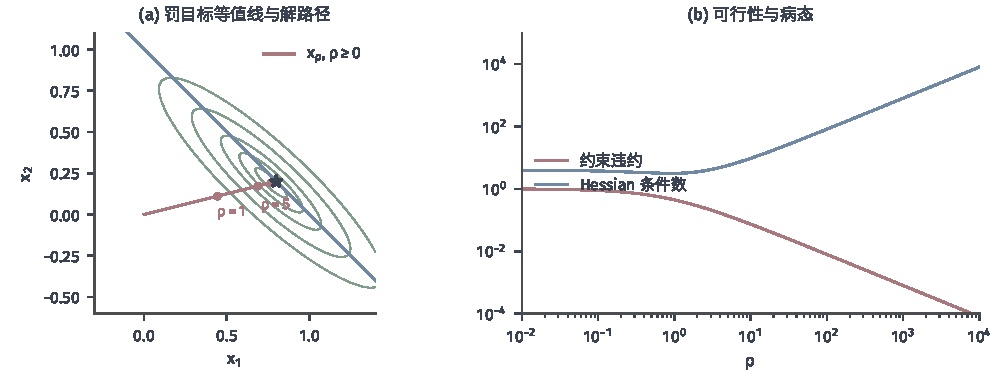
\includegraphics[width=169mm]{figures/03-optimization-evolution-and-signals/01-optimization/matplotlib/c5-penalty-path/figure.pdf}
  \caption{等式二次例的二次惩罚。(a) 绿色椭圆为$\rho=20$时罚目标$Q_\rho$的等值线，沿约束线（蓝）被拉长；红线为解路径$\bm x_\rho=(4\rho,\rho)^\top/(4+5\rho)$，红点标出$\rho=1,5,20$，五角星为约束最优点$(4/5,1/5)^\top$。(b) 对数坐标下，约束违约$4/(4+5\rho)$随$\rho$下降（红），而Hessian条件数（蓝）在$\rho$较大时约按$0.8\rho$增长。}
  \label{fig:opt-con-penalty-path}
\end{figure*}

\subsection{精确惩罚法}
\label{sec:opt-con-exact-penalty}

\paragraph{用违约的绝对值计价}
二次惩罚在可行点附近违约很小时罚得很轻：违约$\delta$只付出$\rho\delta^2/2$，而目标可能因违约获得$|\nu|\delta$量级的好处，所以有限的$\rho$总会接受一点违约。改用违约的一次方计价，
\begin{equation}
\label{eq:opt-con-exact-penalty}
  \Phi_\rho(\bm x)=f(\bm x)+\rho V(\bm x),\qquad
  V(\bm x)=\sum_j|h_j(\bm x)|+\sum_i[g_i(\bm x)]_+,
\end{equation}
小违约的代价与违约成正比，只要单价$\rho$超过目标从违约中获得的边际好处，违约就不划算。以此为目标的方法称为\term{精确惩罚法}（exact penalty method），“精确”的含义是：在适当的有限$\rho$下，惩罚问题的最小点与原问题的最小点对应。代价是$\Phi_\rho$在约束边界上不可微。

图~\ref{fig:opt-con-exact-penalty}用最简单的例子比较两种计价：$\min x$、约束$1-x\leq0$，解$x^\star=1$，乘子$\lambda^\star=1$。二次惩罚$x+\frac\rho2[1-x]_+^2$的最小点是$1-1/\rho$，永远在可行域外。精确惩罚$x+\rho[1-x]_+$在$x<1$时斜率为$1-\rho$：$\rho<1$时目标向左无下界，$\rho=1$时整段$x\leq1$都是最小点，$\rho>1$时唯一最小点就是$x=1$。阈值恰好是乘子。

\begin{figure*}[!htbp]
  \centering
  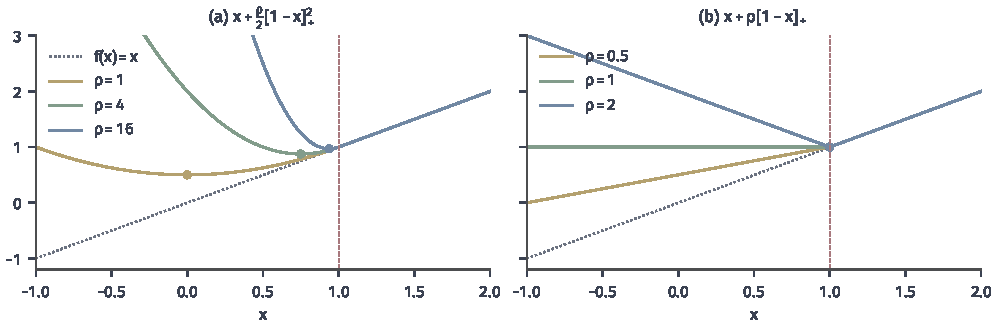
\includegraphics[width=169mm]{figures/03-optimization-evolution-and-signals/01-optimization/matplotlib/c5-exact-penalty/figure.pdf}
  \caption{$\min x$、$1-x\leq0$的两种惩罚，红色竖线为约束边界$x=1$，灰色点线为原目标。(a) 二次惩罚$x+\frac\rho2[1-x]_+^2$，$\rho=1,4,16$时的最小点（圆点）为$1-1/\rho$，都在边界左侧。(b) 精确惩罚$x+\rho[1-x]_+$：$\rho=0.5$时左侧无下界，$\rho=1$时左侧平坦，$\rho=2$时最小点恰为$x=1$。}
  \label{fig:opt-con-exact-penalty}
\end{figure*}

\paragraph{精确性的两条依据}
精确性不是绝对值惩罚的普遍性质，需要条件。第一条依据来自最优乘子。

\begin{theorem}[凸问题的精确惩罚]
\label{thm:opt-con-exact-penalty}
设原问题的强对偶成立，$\bm x^\star$是原问题的最优点，$(\bm\lambda^\star,\bm\nu^\star)$是对偶最优点。若$\rho>\max\{\max_i\lambda_i^\star,\max_j|\nu_j^\star|\}$，则$\bm x^\star$最小化$\Phi_\rho$，且$\Phi_\rho$的每个最小点都可行，因而都是原问题的最优点。
\end{theorem}

\begin{proof}
对任意$\bm x$，$\lambda_i^\star g_i(\bm x)\leq\lambda_i^\star[g_i(\bm x)]_+\leq\rho[g_i(\bm x)]_+$，$\nu_j^\star h_j(\bm x)\leq|\nu_j^\star||h_j(\bm x)|\leq\rho|h_j(\bm x)|$，所以
\[
  \Phi_\rho(\bm x)\geq\mathcal L(\bm x,\bm\lambda^\star,\bm\nu^\star)\geq q(\bm\lambda^\star,\bm\nu^\star)=f(\bm x^\star)=\Phi_\rho(\bm x^\star).
\]
若$\bm x$不可行，则某个$[g_i(\bm x)]_+>0$或$|h_j(\bm x)|>0$，对应项的第二个不等号因$\rho$严格大于乘子而严格成立，$\Phi_\rho(\bm x)>\Phi_\rho(\bm x^\star)$。所以最小点都可行，在可行点上$\Phi_\rho=f$，它们都是原问题的最优点。
\end{proof}

等式二次例中$|\nu^\star|=4/5$，所以$\rho>4/5$时$f+\rho|x_1+x_2-1|$的最小点就是$(4/5,1/5)^\top$。定理只是充分条件，且依赖强对偶与乘子存在；没有这些，绝对值惩罚不必精确。

第二条依据是局部的误差界，它不要求凸性。设在区域$\Omega$内$f$是$K$-Lipschitz的，且每个$\bm x\in\Omega$都有可行点$\bm p\in\Omega$满足$\lVert\bm p-\bm x\rVert_2\leq\kappa V(\bm x)$（违约量控制到可行域的距离）。则
\[
  \Phi_\rho(\bm x)=f(\bm x)+\rho V(\bm x)\geq f(\bm p)-K\kappa V(\bm x)+\rho V(\bm x)=\Phi_\rho(\bm p)+(\rho-K\kappa)V(\bm x),
\]
$\rho>K\kappa$时任何不可行点都严格劣于它的可行修复点，$\Phi_\rho$在$\Omega$中的最小点必可行。这里阈值由误差界常数和Lipschitz常数决定，结论只在$\Omega$内成立。此外，在满足LICQ和二阶充分条件的严格局部最小点处，$\rho$大于乘子的最大绝对值时，该点也是$\Phi_\rho$的严格局部最小点\scite{math-nocedal2006numerical}；这是局部结论，不保证$\Phi_\rho$没有别的更低的局部最小点。

\paragraph{求解与原约束检查}
$\Phi_\rho$非光滑，需要第~\ref{chap:opt-nonsmooth}章的工具：一般情形用次梯度法；违约项有可计算的邻近映射时用邻近梯度法，例如约束只是变量的上下界时，$\rho[x_k-u_k]_++\rho[l_k-x_k]_+$可逐坐标求邻近映射。但$|h_j(\bm x)|$对一般非线性$h_j$不可分，不能套用软阈值公式。不论用哪种方法，返回前都要按原约束重新检查违约，因为数值上只能得到$\Phi_\rho$的近似最小点，而$\rho$是否已越过阈值事先往往未知；若违约不降，就增大$\rho$。

\paragraph{范数正则与范数约束}
机器学习中常见的正则化$\min f(\bm x)+\lambda\lVert\bm x\rVert_1$与约束形式$\min f(\bm x)$、$\lVert\bm x\rVert_1\leq R$有密切关系，但二者不是同一个问题。用本节的语言，前者是把约束$\lVert\bm x\rVert_1-R\leq0$用乘子$\lambda$计价（常数$-\lambda R$不影响最小点）。两个方向都有条件地成立。若约束问题强对偶成立且最优乘子$\lambda^\star$达到，由定理~\ref{thm:opt-con-zero-gap-kkt}(1)，约束问题的每个最优点都最小化$\mathcal L(\cdot,\lambda^\star)=f+\lambda^\star\lVert\cdot\rVert_1-\lambda^\star R$。反过来，若$\hat{\bm x}$最小化$f+\lambda\lVert\cdot\rVert_1$，令$R=\lVert\hat{\bm x}\rVert_1$，则对任意满足$\lVert\bm x\rVert_1\leq R$的$\bm x$，$f(\bm x)\geq f(\hat{\bm x})+\lambda(R-\lVert\bm x\rVert_1)\geq f(\hat{\bm x})$，$\hat{\bm x}$也解约束问题。

但对应关系不是一一的。一维例子$f(x)=\frac12(x-3)^2$：约束$|x|\leq R$的解为$x=\min\{3,R\}$，$0<R<3$时乘子为$3-R$；正则问题的解为软阈值$x=[3-\lambda]_+$。于是$0<R<3$与$0<\lambda<3$之间有$\lambda=3-R$的一一对应，但$R=0$对应全部$\lambda\geq3$，全部$R\geq3$都对应$\lambda=0$。非凸问题中还可能有对偶间隙，此时某些半径根本找不到对应的正则系数。

\section{乘子法与分解}
\label{sec:opt-con-multipliers}

二次惩罚中，$\rho h(\bm x_\rho)$逐渐逼近最优乘子；乘子在第~\ref{sec:opt-con-duality}节又是对偶问题的变量。这提示另一种求解方式：不靠把罚参数推向无穷，而是用约束残差去调整乘子，让乘子“学会”每条约束应有的价格。本节先建立最基本的对偶更新，并说明目标可分时它怎样把大问题拆成独立的小问题；再在Lagrange函数中加入平方违约项，得到收敛更稳健的增广Lagrange法；最后沿着增广模型把变量分成两块交替更新，得到ADMM。后两小节是前后相接的两步构造。

\subsection{对偶上升与对偶分解}
\label{sec:opt-con-dual-ascent}

\paragraph{约束残差是对偶函数的超梯度}
对偶函数$q$是凹函数，最大化它即求解对偶问题。所需的“梯度”在计算$q$时顺带得到。

\begin{theorem}[残差给出超梯度]
\label{thm:opt-con-dual-supergradient}
设$\bm x(\bm\lambda,\bm\nu)$是$\mathcal L(\cdot,\bm\lambda,\bm\nu)$的一个精确最小点。则对所有$\bm\lambda'\geq\bm0$与$\bm\nu'$，
\[
  q(\bm\lambda',\bm\nu')\leq q(\bm\lambda,\bm\nu)+\langle\bm g(\bm x),\bm\lambda'-\bm\lambda\rangle+\langle\bm h(\bm x),\bm\nu'-\bm\nu\rangle,\qquad\bm x=\bm x(\bm\lambda,\bm\nu).
\]
即约束残差$(\bm g(\bm x),\bm h(\bm x))$是凹函数$q$在$(\bm\lambda,\bm\nu)$处的一个超梯度。
\end{theorem}

\begin{proof}
$q(\bm\lambda',\bm\nu')\leq\mathcal L(\bm x,\bm\lambda',\bm\nu')=\mathcal L(\bm x,\bm\lambda,\bm\nu)+\langle\bm g(\bm x),\bm\lambda'-\bm\lambda\rangle+\langle\bm h(\bm x),\bm\nu'-\bm\nu\rangle$，而$\mathcal L(\bm x,\bm\lambda,\bm\nu)=q(\bm\lambda,\bm\nu)$。
\end{proof}

于是沿残差方向移动乘子，并把不等式乘子截回非负：
\begin{equation}
\label{eq:opt-con-dual-ascent}
  \begin{aligned}
    \bm x^{(t)}&\in\argmin_{\bm x}\mathcal L(\bm x,\bm\lambda^{(t)},\bm\nu^{(t)}),\\
    \bm\lambda^{(t+1)}&=\bigl[\bm\lambda^{(t)}+\eta\bm g(\bm x^{(t)})\bigr]_+,\qquad
    \bm\nu^{(t+1)}=\bm\nu^{(t)}+\eta\bm h(\bm x^{(t)}).
  \end{aligned}
\end{equation}
这称为\term{对偶上升法}（dual ascent）。它的经济含义很直接：约束被违反（$g_i>0$）时价格上涨，有余量时价格下降、但不低于零。先完整求出本轮内层点，再用它的残差更新乘子，新旧乘子不能混用。

超梯度步不一定提高$q$；它保证的是到对偶最优点的距离在适当步长下减小，第~\ref{chap:opt-nonsmooth}章对次梯度法的分析可以原样用于$-q$：最优乘子存在、残差有界时，取递减或按预算设定的步长，最佳已访问对偶值以$O(1/\sqrt T)$逼近$d^\star$。若$q$可微且梯度Lipschitz，可以用第~\ref{chap:opt-smooth}章的梯度法分析得到逐步上升和更快的速度。下面是一种常见的充分条件：$f$可微且$\mu$强凸，约束只有仿射等式$\bm A\bm x=\bm b$。此时内层解唯一，且对两组乘子$\bm\nu_1,\bm\nu_2$的内层解$\bm x_1,\bm x_2$，由$\nabla f(\bm x_k)=-\bm A^\top\bm\nu_k$与强凸性，
\[
  \begin{aligned}
    \mu\lVert\bm x_1-\bm x_2\rVert_2^2&\leq\langle\nabla f(\bm x_1)-\nabla f(\bm x_2),\bm x_1-\bm x_2\rangle
    =-\langle\bm\nu_1-\bm\nu_2,\bm A(\bm x_1-\bm x_2)\rangle\\
    &\leq\lVert\bm A\rVert_2\lVert\bm\nu_1-\bm\nu_2\rVert_2\lVert\bm x_1-\bm x_2\rVert_2,
  \end{aligned}
\]
所以内层解关于乘子$\lVert\bm A\rVert_2/\mu$-Lipschitz。可以进一步证明$q$可微，$\nabla q(\bm\nu)=\bm A\bm x(\bm\nu)-\bm b$，其Lipschitz常数不超过$\lVert\bm A\rVert_2^2/\mu$\scite{math-boyd2004convex}，于是步长$\eta\leq\mu/\lVert\bm A\rVert_2^2$保证$q$单调上升。仅凸的$f$可能使内层解不唯一，甚至使$q=-\infty$（例如$f$是线性函数时），这时残差只是一个超梯度，需要按非光滑情形处理。

\begin{example}[等式二次例的对偶上升]
\label{ex:opt-con-dual-ascent}
等式二次例中$\mu=1$、$\lVert\bm A\rVert_2^2=2$，上面的步长条件为$\eta\leq1/2$，取$\eta=0.4$。内层解为$\bm x(\nu)=(-\nu,-\nu/4)^\top$，残差$h=-\frac54\nu-1$，更新$\nu^{(t+1)}=\nu^{(t)}+0.4h$等价于$\nu^{(t+1)}+\frac45=\frac12(\nu^{(t)}+\frac45)$。从$\nu^{(0)}=0$出发，乘子依次为$0,-0.4,-0.6,-0.7,\dots$，误差每步减半；内层点依次为$(0,0)^\top$、$(0.4,0.1)^\top$、$(0.6,0.15)^\top$，残差为$-1,-0.5,-0.25$。所有内层点都不可行，对偶值$q(\nu^{(t)})$却单调升向$2/5$。
\end{example}

例子揭示了对偶上升的一个基本事实：它改善的是对偶下界，内层点在收敛之前通常不可行，原目标也不一定逐步下降。内层点只是“在当前价格下最划算的选择”。要得到原始可行的候选，需要另外的恢复步骤，例如把内层点投影到可行域，或者对内层点作平均；恢复后的可行点与当前对偶值一起构成式~\eqref{eq:opt-con-gap-certificate}的证书。若内层只能近似求解，残差方向带有误差，可信下界还必须按第~\ref{sec:opt-con-weak-duality}小节扣除内层误差。

\paragraph{目标可分时的对偶分解}
对偶上升真正的用处在于分解。设变量分成若干块，目标可分而约束把它们耦合起来：
\[
  \min_{\bm x_1,\dots,\bm x_K}\ \sum_{k=1}^Kf_k(\bm x_k)\quad\text{s.t.}\quad\sum_{k=1}^K\bm A_k\bm x_k=\bm b.
\]
固定乘子$\bm\nu$后，$\mathcal L=\sum_k\bigl(f_k(\bm x_k)+\bm\nu^\top\bm A_k\bm x_k\bigr)-\bm\nu^\top\bm b$按块分离，$K$个内层问题可以独立甚至并行求解；协调者只需收集各块的$\bm A_k\bm x_k$，计算总残差并更新价格。这种做法称为\term{对偶分解}（dual decomposition）。分解改变的是计算的组织方式，求解的仍是同一个对偶问题，收敛性质与普通对偶上升相同。

一致性约束是最常见的耦合。考虑$\min_wr(w)+s(w)$，其中$r(w)=\frac12(w-1)^2$、$s(w)=\frac12(w+1)^2$，最优点$w^\star=0$、最优值$1$。给两项各配一个副本，改写为$\min r(u)+s(v)$、$u-v=0$。固定乘子$\nu$，$\mathcal L=r(u)+s(v)+\nu(u-v)$的两个内层解为$u=1-\nu$、$v=\nu-1$，对偶函数$q(\nu)=2\nu-\nu^2$，最优乘子$\nu^\star=1$。取$\eta=1/4$，更新$\nu^{(t+1)}=\nu^{(t)}+\frac14(u-v)$给出$\nu^{(t)}=1-2^{-t}$、$u^{(t)}=2^{-t}$、$v^{(t)}=-2^{-t}$：两个副本从两侧逼近$0$，但每一轮都不一致。取平均$(u^{(t)}+v^{(t)})/2=0$恢复出可行点，上界为$1$，与下界$q(\nu^{(t)})=1-4^{-t}$的间隙为$4^{-t}$。平均恰好给出最优点是由本例的对称性决定的，不是一般规律。

步长的依据随内层结构变化：$r,s$分别$\mu_r,\mu_s$强凸时，残差$u(\nu)-v(\nu)$关于$\nu$的Lipschitz常数不超过$1/\mu_r+1/\mu_s$，可以据此取常数步长；仅凸时只能按非光滑超梯度方法选择递减步长，并对内层点作平均来恢复原始解。

\subsection{增广Lagrange法}
\label{sec:opt-con-augmented-lagrangian}

\paragraph{在Lagrange函数中加入平方违约}
对偶上升要求内层$\min_{\bm x}\mathcal L$有良好的解，$f$不强凸时这往往做不到；二次惩罚的内层性质好，却要$\rho\to\infty$。把两者结合：对等式约束问题$\min f(\bm x)$、$\bm h(\bm x)=\bm0$，定义增广Lagrange函数
\begin{equation}
\label{eq:opt-con-augmented-lagrangian}
  \mathcal L_\rho(\bm x,\bm\nu)=f(\bm x)+\bm\nu^\top\bm h(\bm x)+\frac\rho2\lVert\bm h(\bm x)\rVert_2^2.
\end{equation}
平方项让内层在约束法向上有正曲率，乘子项负责累计约束的反作用。交替地最小化$\mathcal L_\rho$并更新乘子，就是\term{增广Lagrange法}（augmented Lagrangian method），也称乘子法。

\begin{algorithm}[增广Lagrange法（等式约束）]
\label{alg:opt-con-augmented-lagrangian}
\begin{algorithmic}[1]
\Require 初值$\bm x^{(0)}$、$\bm\nu^{(0)}$，罚参数$\rho>0$，内层容差序列$\epsilon_t$，停止容差
\Ensure 候选$(\bm x^{(t)},\bm\nu^{(t+1)})$
\For{$t=0,1,2,\dots$}
  \State 从$\bm x^{(t-1)}$热启动，近似求解$\min_{\bm x}\mathcal L_\rho(\bm x,\bm\nu^{(t)})$，得$\bm x^{(t)}$
  \State 内层停止条件：$\lVert\nabla_{\bm x}\mathcal L_\rho(\bm x^{(t)},\bm\nu^{(t)})\rVert_2\leq\epsilon_t$
  \State 更新乘子$\bm\nu^{(t+1)}=\bm\nu^{(t)}+\rho\bm h(\bm x^{(t)})$
  \State 若原始残差$\lVert\bm h(\bm x^{(t)})\rVert_2$与驻点残差均低于容差，停止；若残差下降不足，可增大$\rho$
\EndFor
\end{algorithmic}
\end{algorithm}

乘子更新的步长取为$\rho$并非随意。内层驻点满足$\nabla f+\nabla\bm h^\top(\bm\nu^{(t)}+\rho\bm h)=\bm0$（精确求解时），与原问题的驻点条件$\nabla f+\nabla\bm h^\top\bm\nu=\bm0$对照，括号中的$\bm\nu^{(t)}+\rho\bm h(\bm x^{(t)})$正好是新的乘子估计。这也给出一个有用的恒等式：$\nabla_{\bm x}\mathcal L_\rho(\bm x^{(t)},\bm\nu^{(t)})=\nabla_{\bm x}\mathcal L(\bm x^{(t)},\bm\nu^{(t+1)})$，内层容差$\epsilon_t$直接就是原问题KKT条件中驻点性的残差。

\paragraph{为何不必让罚参数趋于无穷}
设原问题凸，$(\bm x^\star,\bm\nu^\star)$满足KKT条件。$\bm x^\star$最小化凸函数$\mathcal L(\cdot,\bm\nu^\star)$；平方项在$\bm x^\star$处为零、在别处非负，所以$\bm x^\star$也最小化$\mathcal L_\rho(\cdot,\bm\nu^\star)$，而且这对\emph{任意}$\rho>0$都成立。只要乘子正确，一个有限的$\rho$就足以让内层给出精确解。二次惩罚相当于始终取$\bm\nu=\bm0$，只能用无限大的$\rho$弥补乘子的缺失。

等式二次例可以算得很清楚。内层驻点方程给出$x_1=-(\nu+\rho r)$、$x_2=-(\nu+\rho r)/4$，其中$r=x_1+x_2-1$，代回得$r=-(4+5\nu)/(4+5\rho)$。乘子更新后
\[
  \nu^{(t+1)}+\frac45=\Bigl(\nu^{(t)}+\frac45\Bigr)\cdot\frac{4}{4+5\rho}.
\]
乘子误差按固定比率$4/(4+5\rho)$线性收缩：$\rho=1$时比率为$4/9$，从$\nu^{(0)}=0$出发乘子依次为$0,-0.444,-0.642,\dots$；$\rho=10$时比率为$4/54\approx0.074$。图~\ref{fig:opt-con-al-multiplier}比较了几种做法。对偶上升与$\rho=1$的增广Lagrange法速度相近；$\rho=10$时每轮误差缩小一个数量级以上。右图把约束违约与二次惩罚对照：二次惩罚的违约只由$\rho$决定，$\rho=1000$时仍有约$8\times10^{-4}$，而增广Lagrange法在固定$\rho$下违约逐轮下降到舍入误差水平。

\begin{figure*}[!htbp]
  \centering
  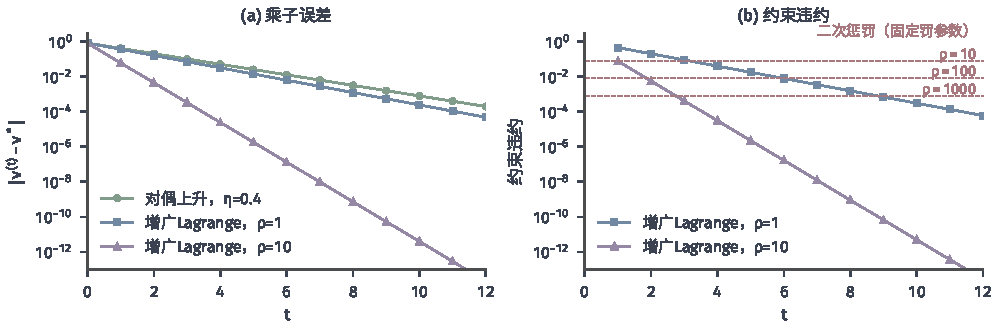
\includegraphics[width=169mm]{figures/03-optimization-evolution-and-signals/01-optimization/matplotlib/c5-al-multiplier/figure.pdf}
  \caption{等式二次例上的乘子更新，均从$\nu^{(0)}=0$出发，对数纵轴。(a) 乘子误差$|\nu^{(t)}-\nu^\star|$：对偶上升（$\eta=0.4$）每步减半；增广Lagrange法的收缩比率为$4/(4+5\rho)$，$\rho=1$时为$4/9$，$\rho=10$时约为$0.074$。(b) 内层点的约束违约：增广Lagrange法在固定$\rho$下持续下降；红色虚线是二次惩罚在$\rho=10,100,1000$时的违约$4/(4+5\rho)$，只能靠增大$\rho$减小。}
  \label{fig:opt-con-al-multiplier}
\end{figure*}

\paragraph{收敛条件与计算代价}
应分别追踪原始残差$\lVert\bm h(\bm x^{(t)})\rVert_2$、驻点残差（即内层容差）与内层求解精度。凸情形下，增广Lagrange法等价于对偶问题上的邻近点法（第~\ref{chap:opt-nonsmooth}章），在对偶最优解存在、内层精确求解时，对任意固定的$\rho>0$乘子都收敛；内层误差需要可求和地减小。一般非凸问题只有局部结论：在满足LICQ和二阶充分条件的局部解附近，$\rho$足够大且初始乘子足够接近时，算法局部收敛\scite{math-nocedal2006numerical}。$\rho$的选择仍是折中：较大的$\rho$让乘子收敛更快，但内层Hessian含$\rho\nabla\bm h^\top\nabla\bm h$，条件数随$\rho$增长，内层求解更难；与二次惩罚的区别在于$\rho$不必无限增大。不等式约束可以先引入松弛变量化为等式，再对松弛变量的非负性作投影。

本小节的内层仍把$\bm x$作为一个整体求解。平方项$\lVert\bm h(\bm x)\rVert_2^2$会把原本可分的变量耦合起来：即使$f$按块可分、约束是$\bm A\bm x+\bm B\bm z=\bm c$这样的线性耦合，$\lVert\bm A\bm x+\bm B\bm z-\bm c\rVert_2^2$也含交叉项，$\bm x$与$\bm z$不能再分开求解。下一小节正是为了恢复可分性而改变这一步。

\subsection{ADMM与一致性约束}
\label{sec:opt-con-admm}

\paragraph{两块交替的增广Lagrange步}
考虑两块可分的目标与线性耦合：
\[
  \min_{\bm x,\bm z}\ f(\bm x)+g(\bm z)\quad\text{s.t.}\quad\bm A\bm x+\bm B\bm z=\bm c.
\]
增广Lagrange函数为$\mathcal L_\rho(\bm x,\bm z,\bm\nu)=f(\bm x)+g(\bm z)+\bm\nu^\top(\bm A\bm x+\bm B\bm z-\bm c)+\frac\rho2\lVert\bm A\bm x+\bm B\bm z-\bm c\rVert_2^2$。增广Lagrange法需要对$(\bm x,\bm z)$联合最小化；\term{交替方向乘子法}（alternating direction method of multipliers，ADMM）只做一轮交替：先固定$\bm z$对$\bm x$最小化，再用新的$\bm x$对$\bm z$最小化，然后更新乘子。用缩放乘子$\bm u=\bm\nu/\rho$书写更简洁：

\begin{algorithm}[ADMM（缩放形式）]
\label{alg:opt-con-admm}
\begin{algorithmic}[1]
\Require $\bm z^{(0)}$、$\bm u^{(0)}$，罚参数$\rho>0$，容差$\epsilon_{\mathrm{pri}}$、$\epsilon_{\mathrm{dual}}$
\Ensure $(\bm x^{(t)},\bm z^{(t)},\rho\bm u^{(t)})$
\For{$t=0,1,2,\dots$}
  \State $\bm x^{(t+1)}=\argmin_{\bm x}\ f(\bm x)+\frac\rho2\lVert\bm A\bm x+\bm B\bm z^{(t)}-\bm c+\bm u^{(t)}\rVert_2^2$
  \State $\bm z^{(t+1)}=\argmin_{\bm z}\ g(\bm z)+\frac\rho2\lVert\bm A\bm x^{(t+1)}+\bm B\bm z-\bm c+\bm u^{(t)}\rVert_2^2$
  \State $\bm u^{(t+1)}=\bm u^{(t)}+\bm A\bm x^{(t+1)}+\bm B\bm z^{(t+1)}-\bm c$
  \State 原始残差$\bm r=\bm A\bm x^{(t+1)}+\bm B\bm z^{(t+1)}-\bm c$，对偶残差$\bm s=\rho\bm A^\top\bm B(\bm z^{(t+1)}-\bm z^{(t)})$；若$\lVert\bm r\rVert_2\leq\epsilon_{\mathrm{pri}}$且$\lVert\bm s\rVert_2\leq\epsilon_{\mathrm{dual}}$，停止
\EndFor
\end{algorithmic}
\end{algorithm}

$\bm x$步使用旧的$\bm z^{(t)}$，$\bm z$步使用刚算出的$\bm x^{(t+1)}$，次序不能对调成同时更新。对偶残差的形式来自$\bm z$步的最优性条件：精确的$\bm z$步使$(\bm x^{(t+1)},\bm z^{(t+1)},\bm\nu^{(t+1)})$满足关于$\bm z$的驻点条件，而关于$\bm x$的驻点条件恰好差$\bm s$。

\paragraph{分裂平方损失与正则项}
以$\ell_1$正则最小二乘为例：$f(\bm x)=\frac12\lVert\bm A\bm x-\bm b\rVert_2^2$、$g(\bm z)=\lambda\lVert\bm z\rVert_1$、约束$\bm x-\bm z=\bm0$。$\bm x$步是一个岭回归式的线性方程$(\bm A^\top\bm A+\rho\bm I)\bm x=\bm A^\top\bm b+\rho(\bm z^{(t)}-\bm u^{(t)})$，系数矩阵不随迭代变化，分解一次即可重复使用；$\bm z$步是第~\ref{chap:opt-nonsmooth}章的软阈值$\bm z=S_{\lambda/\rho}(\bm x^{(t+1)}+\bm u^{(t)})$。两个子问题各自只处理一种结构，这正是分裂的目的。

取最简单的标量情形$f(x)=\frac12(x-3)^2$、$g(z)=|z|$、约束$x=z$，最优解为软阈值$x^\star=z^\star=2$，最优乘子$\nu^\star=1$。取$\rho=1$，从$z=u=0$出发：$x$步$x=(3+z-u)/2=1.5$，$z$步$z=S_1(x+u)=0.5$，$u=u+x-z=1$；第二轮$x=(3+0.5-1)/2=1.25$，$z=S_1(2.25)=1.25$，$u=1$；第三轮$x=1.625$，$z=1.625$。此后$u$保持为$1=\nu^\star/\rho$，$x$与$z$相等，与$2$的距离每轮减半。图~\ref{fig:opt-con-admm}(a)在$(x,z)$平面上画出这条路径：$x$步沿水平方向移动，$z$步沿竖直方向移动，两种移动交替，逐渐收拢到约束线$x=z$上的最优点。图(b)比较不同$\rho$：在$u$稳定以后，本例的误差收缩比率为$\rho/(1+\rho)$，较小的$\rho$反而更快；一般问题中$\rho$同时影响原始残差与对偶残差的平衡，没有普遍最优的取值。

\begin{figure*}[!htbp]
  \centering
  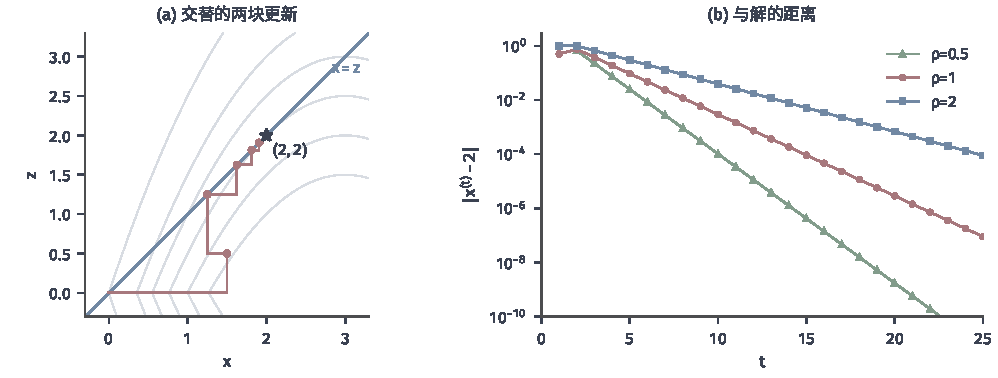
\includegraphics[width=169mm]{figures/03-optimization-evolution-and-signals/01-optimization/matplotlib/c5-admm/figure.pdf}
  \caption{标量问题$\min\frac12(x-3)^2+|z|$、$x=z$上的ADMM。(a) $\rho=1$，从$z=u=0$出发；灰色曲线为$\frac12(x-3)^2+|z|$的等值线，蓝线为约束$x=z$。红色折线中水平段是$x$步，竖直段是$z$步，红点为每轮结束时的$(x,z)$，收拢到五角星$(2,2)$。(b) 误差$|x^{(t)}-2|$（对数纵轴）在$\rho=0.5,1,2$下的变化；乘子稳定后误差按$\rho/(1+\rho)$收缩。本例中第二轮起$z^{(t)}=x^{(t)}$，原始残差恰为零。}
  \label{fig:opt-con-admm}
\end{figure*}

\paragraph{保证与适用范围}
ADMM的标准保证需要以下条件：$f,g$是闭适当凸函数；未增广的Lagrange函数$\mathcal L_0$有鞍点；两个子问题能精确求解（或误差可求和）。在这些条件下，原始残差$\bm r^{(t)}\to\bm0$，目标值$f(\bm x^{(t)})+g(\bm z^{(t)})\to f^\star$，乘子$\bm\nu^{(t)}$收敛到对偶最优解\scite{boyd2011admm}。注意这里没有断言$(\bm x^{(t)},\bm z^{(t)})$本身收敛；迭代点列的收敛需要额外条件（例如$\bm A,\bm B$列满秩），使用时要另行核查。收敛速度一般只是次线性的，适合中等精度的求解。

ADMM最适合一致性形式的问题：$\min\sum_{k=1}^Kf_k(\bm x_k)+g(\bm z)$、$\bm x_k=\bm z$。$\bm x$步对各$k$完全分离，可以在$K$台机器上并行；每轮通信只需收集$\bm x_k+\bm u_k$，在中心求$\bm z$（$g=0$时就是取平均），再广播回去。与对偶分解相比，它的每个子问题都含平方项，对仅凸的$f_k$也有良好定义，代价是子问题多了一个二次项。直接把两块的交替推广到三块或更多块，即使问题凸，也可能发散\scite{chen2016admm}；非凸问题中的ADMM也没有同样的保证，需要针对具体结构另作分析。

\section{序列二次规划}
\label{sec:opt-con-sqp}

惩罚法与乘子法把约束问题变成一串无约束问题，每个内层问题本身还要迭代很多步。对光滑的非线性约束问题，还可以像第~\ref{chap:opt-smooth}章的牛顿法那样，直接在当前点建立一个局部模型，一步解出模型的最优步。约束问题的局部模型是一个二次规划：目标用二阶信息近似，约束用一阶信息线性化。本节先说明这个子问题怎样构造、求解时会遇到什么障碍；再说明模型给出的步怎样放回原问题检验，以及在什么条件下这一方法收敛得很快。它与第~\ref{sec:opt-con-interior-point}节沿可行域内部路径前进的内点法是两种不同的思路。

\subsection{局部二次子问题}
\label{sec:opt-con-sqp-subproblem}

\paragraph{子问题的构造}
设当前迭代为$\bm x^{(t)}$，乘子估计为$(\bm\lambda^{(t)},\bm\nu^{(t)})$，以步向量$\bm p$为未知量。约束线性化为$h_j(\bm x^{(t)})+\langle\nabla h_j(\bm x^{(t)}),\bm p\rangle=0$与$g_i(\bm x^{(t)})+\langle\nabla g_i(\bm x^{(t)}),\bm p\rangle\leq0$；目标取一阶项加上Lagrange函数的曲率：
\begin{equation}
\label{eq:opt-con-sqp-subproblem}
  \min_{\bm p}\ \langle\nabla f(\bm x^{(t)}),\bm p\rangle+\frac12\bm p^\top\bm H_t\bm p
  \quad\text{s.t.}\quad
  \bm h+\bm J_h\bm p=\bm0,\quad\bm g+\bm J_g\bm p\leq\bm0,
\end{equation}
其中$\bm h,\bm g$与Jacobian $\bm J_h,\bm J_g$都在$\bm x^{(t)}$处取值，$\bm H_t=\nabla^2_{\bm x\bm x}\mathcal L(\bm x^{(t)},\bm\lambda^{(t)},\bm\nu^{(t)})$或它的拟牛顿近似。这是第~\ref{sec:opt-con-qp}小节定义的二次规划。逐项看：目标梯度决定一阶下降方向；约束残差$\bm h,\bm g$决定线性化约束要求步子修正多少违约；Jacobian决定约束怎样随步子变化；曲率用的是$\nabla^2\mathcal L$而不是$\nabla^2f$，因为沿弯曲的约束面移动时，约束的曲率也会改变目标值，乘子把这部分曲率加了进来。子问题的乘子就是下一轮的乘子估计。反复求解这样的子问题称为\term{序列二次规划}（sequential quadratic programming，SQP）。

\paragraph{等式约束：KKT线性系统}
只有等式约束时，子问题的KKT条件是线性方程组
\begin{equation}
\label{eq:opt-con-sqp-kkt}
  \begin{bmatrix}\bm H_t&\bm J_h^\top\\\bm J_h&\bm0\end{bmatrix}
  \begin{bmatrix}\bm p\\\bm\nu^{(t+1)}\end{bmatrix}
  =-\begin{bmatrix}\nabla f(\bm x^{(t)})\\\bm h(\bm x^{(t)})\end{bmatrix}.
\end{equation}
它恰好是对原问题的KKT方程组$\nabla f+\bm J_h^\top\bm\nu=\bm0$、$\bm h=\bm0$作一步牛顿线性化的结果（在$\bm H_t$取精确Hessian时），所以SQP可以看作对KKT条件使用牛顿法。

考虑$\min x_1+x_2$、约束$x_1^2+x_2^2=2$。最优点$\bm x^\star=(-1,-1)^\top$，由$(1,1)^\top+\nu(2x_1,2x_2)^\top=\bm0$得$\nu^\star=1/2$。$\nabla^2_{\bm x\bm x}\mathcal L=2\nu\bm I$。从$\bm x^{(0)}=(0.2,-1.6)^\top$、$\nu^{(0)}=1$出发：$h=0.04+2.56-2=0.6$，$\bm J_h=(0.4,-3.2)$，$\bm H_0=2\bm I$。方程组第一行给出$\bm p=-\frac12\bigl((1,1)^\top+\nu^{(1)}(0.4,-3.2)^\top\bigr)$，代入第二行$\bm J_h\bm p=-0.6$得$-\frac12(-2.8+10.4\nu^{(1)})=-0.6$，于是$\nu^{(1)}=4/10.4\approx0.385$，$\bm p\approx(-0.577,0.115)^\top$，$\bm x^{(1)}\approx(-0.377,-1.485)^\top$。图~\ref{fig:opt-con-sqp}画出后续迭代：第一个子问题的线性化约束（黄色虚线）是圆在$\bm x^{(0)}$附近的切线方向平移，新点落在这条直线上而不在圆上；之后迭代很快靠近最优点，约束值依次为$0.6,0.346,0.897,0.076,8\times10^{-4},\dots$，前几步并不单调，进入最优点附近后每步误差大致平方。

\begin{figure}[!htbp]
  \centering
  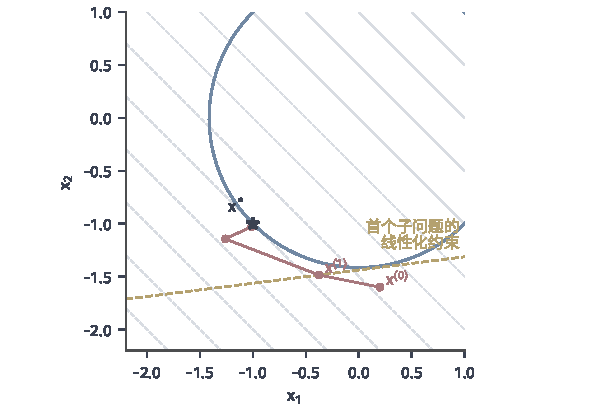
\includegraphics[width=100mm]{figures/03-optimization-evolution-and-signals/01-optimization/matplotlib/c5-sqp/figure.pdf}
  \caption{$\min x_1+x_2$、$x_1^2+x_2^2=2$上的SQP迭代（精确Lagrange Hessian，全步长）。蓝色圆为可行域，灰色虚线为目标等值线，黄色虚线为第一个子问题的线性化约束。红色折线从$\bm x^{(0)}=(0.2,-1.6)^\top$出发，约5步到达五角星$\bm x^\star=(-1,-1)^\top$；中间迭代点不在圆上。}
  \label{fig:opt-con-sqp}
\end{figure}

\paragraph{不等式与活动集}
含不等式时，子问题~\eqref{eq:opt-con-sqp-subproblem}要用二次规划方法求解（如第~\ref{sec:opt-con-qp}小节的活动集思路），它在线性化约束中选出当前需要以等号处理的那些。在满足严格互补等条件的解附近，子问题选出的活动集与原问题最优点的活动集相同，此后SQP就像在固定活动集上的等式约束牛顿法；远离解时，活动集可能在相邻迭代之间反复变化。

\paragraph{子问题可能不可用}
子问题不是每次都能直接给出一个好步。第一种障碍是曲率：若$\bm H_t$在线性化约束的零空间上不正定，二次规划可能无下界或只有鞍点。$\nabla^2\mathcal L$在远离解处完全可能不定，例如上例若乘子估计为负，$2\nu\bm I$就是负定的。常用的修正是给$\bm H_t$加上$\delta\bm I$直到零空间上正定，或者用保持正定的拟牛顿更新（如阻尼BFGS，第~\ref{chap:opt-smooth}章）代替精确Hessian。第二种障碍是线性化约束本身无解。仍看上例，若在原点处线性化，$\bm J_h=(0,0)$、$h=-2$，线性化约束成为$0=2$，子问题不可行，而原问题是可行的。这时需要可行性恢复：暂时改为最小化线性化约束的违约（例如引入松弛变量的弹性子问题），先回到线性化相容的区域。两种障碍都意味着不能默认每轮都得到可以直接采用的下降步。

\subsection{模型步的接受与收敛}
\label{sec:opt-con-sqp-acceptance}

\paragraph{用评价函数检验模型步}
子问题的解只在模型里最优。把$\bm x^{(t)}+\bm p$放回原问题时，目标可能变差、约束违约也可能变大（上例第二步约束值就从$0.346$升到$0.897$）。目标与约束可能朝相反方向变化，需要一个同时计量两者的标准。常用的是第~\ref{sec:opt-con-exact-penalty}小节的精确罚函数，在这里称为\term{评价函数}（merit function）：
\[
  \phi_\rho(\bm x)=f(\bm x)+\rho\lVert\bm h(\bm x)\rVert_1+\rho\sum_i[g_i(\bm x)]_+.
\]
沿步向量回溯：从$\alpha=1$开始，若$\phi_\rho(\bm x^{(t)}+\alpha\bm p)\leq\phi_\rho(\bm x^{(t)})+c\,\alpha D$（$c\in(0,1)$，$D$为$\phi_\rho$沿$\bm p$的方向导数）就接受，否则把$\alpha$减半。

$\bm p$确实是$\phi_\rho$的下降方向需要条件。以等式约束为例，$\bm p$满足$\bm J_h\bm p=-\bm h$，所以$\lVert\bm h\rVert_1$沿$\bm p$的方向导数为$-\lVert\bm h\rVert_1$；由式~\eqref{eq:opt-con-sqp-kkt}第一行，$\nabla f^\top\bm p=-\bm p^\top\bm H_t\bm p-(\bm\nu^{(t+1)})^\top\bm J_h\bm p=-\bm p^\top\bm H_t\bm p+(\bm\nu^{(t+1)})^\top\bm h$。于是
\[
  D=\nabla f^\top\bm p-\rho\lVert\bm h\rVert_1\leq-\bm p^\top\bm H_t\bm p-\bigl(\rho-\lVert\bm\nu^{(t+1)}\rVert_\infty\bigr)\lVert\bm h\rVert_1.
\]
当$\bm H_t$在相应方向上正定且$\rho\geq\lVert\bm\nu^{(t+1)}\rVert_\infty$时，$D<0$（除非$\bm p=\bm0$且$\bm h=\bm0$，即已到KKT点）。这再次说明罚参数要超过乘子；实现中每轮检查这一条件，不满足就增大$\rho$。

几种失败各有对应的处理。步子太长、模型在远处不准时，回溯缩短步长。$\rho$太小、方向不是评价函数的下降方向时，增大$\rho$。线性化不相容或连续多次回溯失败时，进入可行性恢复阶段。还有一种接近解时才出现的情形：全步长本已很好，却因约束的曲率使评价函数略升而被拒绝，导致收敛变慢，称为Maratos效应；常见的补救是加一个二阶校正步，再检验评价函数\scite{math-nocedal2006numerical}。整个过程中应记录的是原问题的原始可行性$\lVert\bm h\rVert$、$[\bm g]_+$与驻点残差$\lVert\nabla_{\bm x}\mathcal L\rVert$，而不是“二次子问题已解”。

\paragraph{局部快速收敛及其条件}
SQP的吸引力在于解附近的速度。设$\bm x^\star$是局部最小点，满足LICQ、二阶充分条件（$\nabla^2_{\bm x\bm x}\mathcal L$在活跃约束梯度的零空间上正定）与严格互补，各函数二阶连续可微。若初值与初始乘子足够接近$(\bm x^\star,\bm\lambda^\star,\bm\nu^\star)$且使用精确Hessian和全步长，SQP二次收敛；若用拟牛顿近似$\bm H_t$，在近似沿相关方向逐渐准确的条件下超线性收敛\scite{math-nocedal2006numerical}。这些条件正是引理~\ref{lem:opt-con-kkt-matrix}中让KKT矩阵可逆的条件：牛顿法在KKT方程组的非退化解附近二次收敛。上例中到最优点的距离从$\bm x^{(3)}$的约$2.9\times10^{-2}$依次降到$5.1\times10^{-4}$、$3.9\times10^{-7}$、$1.1\times10^{-13}$，每步大致平方，正是这种二次收敛。

代价方面，每轮需要梯度、约束Jacobian、Lagrange Hessian（或其近似）以及一次二次规划求解。等式约束时后者是一次KKT线性系统的分解；变量多而稀疏时可以用迭代法近似求解，此时子问题只给出近似步，局部速度相应下降，需要按不精确牛顿法的方式控制线性系统残差。还要强调，这些都是局部结论。“收敛到一个满足KKT条件的点”与“从任意初值得到全局最优”是两回事：非凸问题中即使每个二次子问题都精确求解，SQP也只能找到局部解或驻点。

\section{内点法}
\label{sec:opt-con-interior-point}

活动集法与SQP都要判断哪些不等式在最优点活跃，这个组合选择在约束很多时可能代价很高。\term{内点法}（interior-point method）换了一个角度：始终待在不等式约束严格成立的内部，用一个在边界处趋于无穷的障碍项阻止迭代越界，再逐步减弱障碍，让迭代沿一条光滑曲线滑向最优点。本节先在线性规划上建立这条曲线——中心路径，然后区分两种沿路径前进的方法：先固定障碍参数把子问题解好再减小参数的障碍法，以及把原始与对偶变量放在一起作牛顿更新的原始—对偶内点法。本节用$\mu>0$表示障碍参数（与强凸常数无关），标准型线性规划$\min\bm c^\top\bm x$、$\bm A\bm x=\bm b$、$\bm x\geq\bm0$中$\bm A\in\mathbb R^{m\times n}$，变量个数为$n$。

\subsection{障碍函数与中心路径}
\label{sec:opt-con-central-path}

\paragraph{对数障碍}
不等式$x_j\geq0$要求迭代不能越过$x_j=0$。若在目标中加入$-\mu\log x_j$，它在$x_j\downarrow0$时趋于$+\infty$，迭代就不会碰到边界；$\mu$越小，障碍对内部的影响越弱。对满行秩的标准型线性规划，构造\term{对数障碍函数}（logarithmic barrier function）问题
\begin{equation}
\label{eq:opt-con-barrier-lp}
  \min_{\bm x}\ B_\mu(\bm x)=\bm c^\top\bm x-\mu\sum_{j=1}^n\log x_j\quad\text{s.t.}\quad\bm A\bm x=\bm b,\ \bm x>\bm0.
\end{equation}
等式约束仍原样保留。$-\log$严格凸，所以$B_\mu$在可行集上严格凸，最小点若存在则唯一。存在性却不是自动的，它需要原始和对偶两侧都严格可行。

\begin{theorem}[中心点的存在唯一]
\label{thm:opt-con-central-path}
设$\bm A$行满秩，存在$\bm x>\bm0$使$\bm A\bm x=\bm b$（原始严格可行），并存在$\bar{\bm y}$与$\bar{\bm s}>\bm0$使$\bm A^\top\bar{\bm y}+\bar{\bm s}=\bm c$（对偶严格可行）。则对每个$\mu>0$，问题~\eqref{eq:opt-con-barrier-lp}有唯一最小点$\bm x(\mu)$。
\end{theorem}

\begin{proof}
在可行集上，$\bm c^\top\bm x=(\bm A^\top\bar{\bm y}+\bar{\bm s})^\top\bm x=\bm b^\top\bar{\bm y}+\bar{\bm s}^\top\bm x$，于是$B_\mu(\bm x)=\bm b^\top\bar{\bm y}+\sum_j\bigl(\bar s_jx_j-\mu\log x_j\bigr)$。每一项$\bar s_jx_j-\mu\log x_j$在$x_j>0$上有下界$\mu-\mu\log(\mu/\bar s_j)$，并在$x_j\downarrow0$或$x_j\to\infty$时趋于$+\infty$。因此对任意可行$\bm x_0>\bm0$，下水平集$\{\bm x:\bm A\bm x=\bm b,\ \bm x>\bm0,\ B_\mu(\bm x)\leq B_\mu(\bm x_0)\}$中每个坐标都被限制在某个$[\epsilon,M]$内（$\epsilon>0$），它是非空紧集。连续函数在其上达到最小，这就是全局最小点；严格凸性给出唯一性。
\end{proof}

对偶严格可行不能省去。$\min0$、约束$x_1-x_2=0$、$\bm x\geq\bm0$的原问题严格可行，最优值为$0$；但$B_\mu=-\mu\log x_1-\mu\log x_2$沿可行射线$x_1=x_2=s\to\infty$趋于$-\infty$，没有最小点。它的对偶约束$y\leq0$、$-y\leq0$迫使$y=0$、$\bm s=\bm0$，没有严格可行的对偶点。只凭原始严格可行和有限最优值，不能宣称中心路径存在。

\paragraph{中心路径与间隙}
最小点由KKT条件刻画：存在$\bm y$使$\bm c-\mu\bm X^{-1}\bm1-\bm A^\top\bm y=\bm0$，其中$\bm X=\operatorname{diag}(\bm x)$。令$\bm s=\mu\bm X^{-1}\bm1>\bm0$，条件变为
\begin{equation}
\label{eq:opt-con-central-path}
  \bm A\bm x=\bm b,\quad\bm A^\top\bm y+\bm s=\bm c,\quad x_js_j=\mu\ (j=1,\dots,n),\quad\bm x,\bm s>\bm0.
\end{equation}
与线性规划的KKT条件对照，前两组是原始与对偶可行性，第三组本应是互补松弛$x_js_j=0$，现在被“扰动”为$x_js_j=\mu$。当$\mu$从$+\infty$减小到$0$，解$(\bm x(\mu),\bm y(\mu),\bm s(\mu))$画出一条曲线，称为\term{中心路径}（central path）。沿这条路径，原始—对偶间隙可以精确算出：
\[
  \bm c^\top\bm x(\mu)-\bm b^\top\bm y(\mu)=(\bm A^\top\bm y+\bm s)^\top\bm x-(\bm A\bm x)^\top\bm y=\bm s^\top\bm x=n\mu.
\]
$\bm x(\mu)$原始可行，$\bm y(\mu)$对偶可行，由弱对偶，$\bm x(\mu)$的次优性不超过$n\mu$。要得到$\epsilon$精度，只需走到$\mu\leq\epsilon/n$。这个界成立的前提是精确位于中心点；迭代只是近似中心时，还要计入离中心的偏差和内层求解误差。

\begin{example}[两变量的中心路径]
\label{ex:opt-con-central-path}
$\min x_1+2x_2$、$x_1+x_2=1$、$\bm x\geq\bm0$，最优点$(1,0)^\top$，对偶最优$y^\star=1$。由式~\eqref{eq:opt-con-central-path}，$x_j=\mu/(c_j-y)$，代入$x_1+x_2=1$得$\mu(3-2y)=(1-y)(2-y)$。取满足$y<1$的根，$y(\mu)=\bigl(3-2\mu-\sqrt{4\mu^2+1}\bigr)/2$。$\mu=1$时$y\approx-0.618$，$\bm x\approx(0.618,0.382)^\top$，间隙$x_1+2x_2-y=2$；$\mu=0.1$时$y\approx0.890$，$\bm x\approx(0.910,0.090)^\top$，间隙$0.2$。两次都等于$n\mu=2\mu$。$\mu\to0$时$y\to1$、$\bm x\to(1,0)^\top$。
\end{example}

图~\ref{fig:opt-con-central-path}把同一构造放到三个变量上：$\min x_1+2x_2+3x_3$，$x_1+x_2+x_3=1$。可行域是单纯形，画成三角形。$\mu$很大时障碍项主导，中心点接近三角形的重心（解析中心）；$\mu$减小时，中心点沿一条光滑曲线移向最优顶点$\bm e_1$，始终不碰边界。绿色曲线是$\mu=0.3$时障碍目标的等值线：它们在边界附近陡然升高，在内部围出一个“碗”，碗底就是$\bm x(0.3)\approx(0.670,0.207,0.123)^\top$。

\begin{figure}[!htbp]
  \centering
  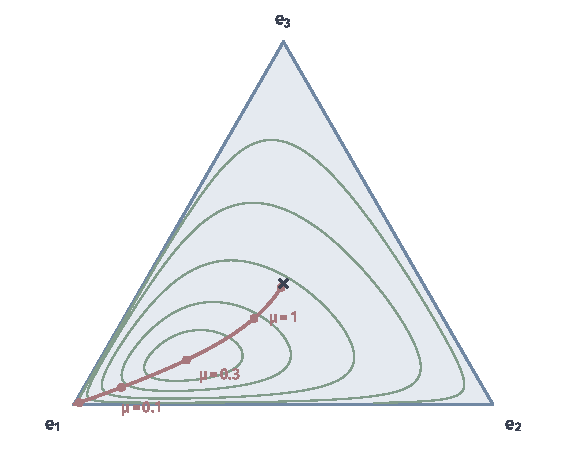
\includegraphics[width=96mm]{figures/03-optimization-evolution-and-signals/01-optimization/matplotlib/c5-central-path/figure.pdf}
  \caption{$\min x_1+2x_2+3x_3$、$x_1+x_2+x_3=1$、$\bm x\geq\bm0$的中心路径，单纯形用重心坐标画成三角形。红色曲线为$\mu$从$10^3$减小到$10^{-3}$的中心点$\bm x(\mu)$，从重心附近（黑叉）出发通向最优顶点$\bm e_1$；红点标出$\mu=10,1,0.3,0.1,0.01$，对应间隙$3\mu$。绿色曲线为$\mu=0.3$时障碍目标$B_\mu$的等值线。}
  \label{fig:opt-con-central-path}
\end{figure}

\subsection{障碍法}
\label{sec:opt-con-barrier-method}

\paragraph{外层减小参数，内层牛顿居中}
\term{障碍法}（barrier method）沿中心路径分段前进：固定$\mu$，用牛顿法把问题~\eqref{eq:opt-con-barrier-lp}解到足够接近中心点；然后把$\mu$缩小一个固定比例，以当前点为热启动，重复。$B_\mu$的梯度为$\bm c-\mu\bm X^{-1}\bm1$，Hessian为$\mu\bm X^{-2}$。在等式约束$\bm A\bm x=\bm b$下，牛顿步$\Delta\bm x$保持$\bm A\Delta\bm x=\bm0$，由线性系统
\[
  \begin{bmatrix}\mu\bm X^{-2}&\bm A^\top\\\bm A&\bm0\end{bmatrix}
  \begin{bmatrix}\Delta\bm x\\\bm w\end{bmatrix}
  =\begin{bmatrix}-(\bm c-\mu\bm X^{-1}\bm1)\\\bm0\end{bmatrix}
\]
确定，这是第~\ref{chap:opt-smooth}章牛顿法加上等式约束的形式，系数矩阵就是式~\eqref{eq:opt-con-kkt-matrix}的KKT矩阵。步长要保持$\bm x>\bm0$：先取使$\bm x+\alpha\Delta\bm x>\bm0$的最大$\alpha$乘以$0.99$之类的系数，再在$B_\mu$上作回溯线搜索。

\begin{algorithm}[障碍法（标准型线性规划）]
\label{alg:opt-con-barrier}
\begin{algorithmic}[1]
\Require 严格可行初值$\bm x>\bm0$（$\bm A\bm x=\bm b$），$\mu_0>0$，缩小因子$\theta\in(0,1)$，精度$\epsilon$，居中容差
\Ensure 近似最优点$\bm x$
\Loop
  \Repeat\Comment{居中：牛顿法求$B_\mu$的最小点}
    \State 解上面的KKT系统得$\Delta\bm x$；取保持$\bm x>\bm0$的步长并在$B_\mu$上回溯；更新$\bm x$
  \Until{牛顿减量$(\Delta\bm x^\top\mu\bm X^{-2}\Delta\bm x)^{1/2}$低于居中容差}
  \If{$n\mu\leq\epsilon$}
    \State 返回$\bm x$
  \EndIf
  \State $\mu\leftarrow\theta\mu$
\EndLoop
\end{algorithmic}
\end{algorithm}

\paragraph{起点与可行性阶段}
算法需要一个严格可行的起点。没有现成的起点时，先求解一个辅助问题，例如$\min_{\bm x,\sigma}\sigma$、$\bm A\bm x=\bm b$、$x_j+\sigma\geq0$：取任意满足$\bm A\bm x=\bm b$的$\bm x$和足够大的$\sigma$，它就是辅助问题的严格可行点。辅助问题的最优值$\sigma^\star<0$时，得到严格可行的起点；$\sigma^\star>0$时，原问题不可行；$\sigma^\star=0$时，原问题可行但没有严格可行点，不满足本节的假设，需要先消去恒为零的变量再处理。这一区分很重要：“原问题不可行”与“可行但不满足严格可行假设”需要不同的报告。

\paragraph{停止、成本与数值问题}
停止由两部分共同决定：外层的$n\mu\leq\epsilon$控制中心点的间隙，居中容差控制当前点离中心点多远。外层迭代次数约为$\log(n\mu_0/\epsilon)/\log(1/\theta)$；每次外层的牛顿步数取决于$\theta$：缩得越猛，外层越少，但每次居中需要的牛顿步越多。每个牛顿步的主要成本是解KKT系统，常消去$\Delta\bm x$得到$m\times m$的正规方程$\bm A\bm X^2\bm A^\top\bm w=\cdots$，稠密时形成需$O(m^2n)$、分解需$O(m^3)$，稀疏时取决于$\bm A$的结构。这三者——外层次数、每次的牛顿步数、每步的线性求解——应分开计量。

利用障碍函数的自协调性质，可以证明短步长的路径跟踪方法至多需要$O(\sqrt n\log(n\mu_0/\epsilon))$次牛顿步\scite{math-boyd2004convex}；这一理论的细节作为补充，不在此展开。实践中观察到的外层次数往往很少，但这只是经验，不能当作统一的成本界。另一个实际问题是数值病态：接近最优点时，最优解为零的那些坐标$x_j\to0$，$\mu\bm X^{-2}$的对应元素约为$s_j^2/\mu\to\infty$，而另一些元素趋于零，KKT系统的条件数随之恶化。成熟的实现依靠专门的分解与正则化处理这一问题，用户至少应检查最终残差，而不是只看算法是否报告收敛。

\paragraph{推广到二阶锥与半正定约束}
同样的思路适用于第~\ref{sec:opt-con-quadratic-conic}节的锥模型，只需换一个在锥内部有定义、在边界处趋于无穷的障碍。二阶锥$\{(\bm u,t):\lVert\bm u\rVert_2\leq t\}$的内部是$t>\lVert\bm u\rVert_2$，取$-\log(t^2-\lVert\bm u\rVert_2^2)$；半正定锥的内部是$\bm X\succ\bm0$，取$-\log\det\bm X$，它的梯度为$-\bm X^{-1}$，Hessian作用在方向$\bm D$上为$\bm X^{-1}\bm D\bm X^{-1}$。中心路径上的间隙不再是变量个数乘$\mu$，而是由障碍决定的常数乘$\mu$：每个二阶锥贡献$2\mu$，每个$k\times k$半正定块贡献$k\mu$（在中心点$\bm X\bm S=\mu\bm I$，间隙$\operatorname{tr}(\bm X\bm S)=k\mu$），所以不能照搬线性规划的$n\mu$。计算上的主要变化在牛顿系统：半正定规划中形成$m\times m$的系数矩阵需要计算$\operatorname{tr}(\bm A_i\bm X\bm A_l\bm X)$，稠密时代价约为$O(mk^3+m^2k^2)$，存储也从向量变为$k\times k$矩阵；问题规模较大时，这往往是半正定规划的瓶颈。

\subsection{原始—对偶内点法}
\label{sec:opt-con-primal-dual-ipm}

\paragraph{对扰动的KKT方程组作牛顿法}
障碍法只把$\bm x$当作迭代变量，乘子是居中后才读出的。另一种做法直接把式~\eqref{eq:opt-con-central-path}看作关于$(\bm x,\bm y,\bm s)$的非线性方程组，并且不必等居中完成就降低目标$\mu$。在当前点$(\bm x,\bm y,\bm s)$（$\bm x,\bm s>\bm0$，不要求满足等式）处，记$\bm r_{\mathrm p}=\bm A\bm x-\bm b$、$\bm r_{\mathrm d}=\bm A^\top\bm y+\bm s-\bm c$、平均互补量$\bar\mu=\bm x^\top\bm s/n$，目标参数取$\sigma\bar\mu$（$\sigma\in(0,1)$），对方程组作牛顿线性化：
\begin{equation}
\label{eq:opt-con-pd-newton}
  \begin{bmatrix}\bm0&\bm A^\top&\bm I\\\bm A&\bm0&\bm0\\\bm S&\bm0&\bm X\end{bmatrix}
  \begin{bmatrix}\Delta\bm x\\\Delta\bm y\\\Delta\bm s\end{bmatrix}
  =-\begin{bmatrix}\bm r_{\mathrm d}\\\bm r_{\mathrm p}\\\bm X\bm S\bm1-\sigma\bar\mu\bm1\end{bmatrix},
\end{equation}
其中$\bm S=\operatorname{diag}(\bm s)$。前两行是线性方程，第三行线性化了$x_js_j=\sigma\bar\mu$。步长取保持$\bm x,\bm s$严格为正的最大步长乘以$0.99$（不超过$1$），原始与对偶变量同步更新。这就是\term{原始—对偶内点法}（primal-dual interior-point method）。与障碍法“先固定参数求中心点，再减小参数”相比，它每轮只走一步牛顿步，就同时改进可行性、互补性和中心性。

\begin{algorithm}[原始—对偶路径跟踪]
\label{alg:opt-con-primal-dual}
\begin{algorithmic}[1]
\Require $(\bm x,\bm y,\bm s)$，$\bm x,\bm s>\bm0$；居中参数$\sigma\in(0,1)$；容差$\epsilon_{\mathrm p},\epsilon_{\mathrm d},\epsilon_{\mathrm g}$
\Ensure 近似原始—对偶最优三元组
\Repeat
  \State 计算$\bm r_{\mathrm p}$、$\bm r_{\mathrm d}$、$\bar\mu=\bm x^\top\bm s/n$
  \State 解式~\eqref{eq:opt-con-pd-newton}得$(\Delta\bm x,\Delta\bm y,\Delta\bm s)$
  \State $\alpha=\min\{1,\ 0.99\cdot\max\{\alpha':\bm x+\alpha'\Delta\bm x\geq\bm0,\ \bm s+\alpha'\Delta\bm s\geq\bm0\}\}$
  \State $(\bm x,\bm y,\bm s)\leftarrow(\bm x,\bm y,\bm s)+\alpha(\Delta\bm x,\Delta\bm y,\Delta\bm s)$
\Until{$\lVert\bm r_{\mathrm p}\rVert\leq\epsilon_{\mathrm p}$，$\lVert\bm r_{\mathrm d}\rVert\leq\epsilon_{\mathrm d}$，$\bm x^\top\bm s\leq\epsilon_{\mathrm g}$}
\end{algorithmic}
\end{algorithm}

\paragraph{三项残差共同决定停止}
图~\ref{fig:opt-con-pdipm}在一个资源分配线性规划上运行算法~\ref{alg:opt-con-primal-dual}。原问题为$\max3x_1+2x_2$、$2x_1+x_2\leq4$、$x_1+2x_2\leq4$，加入松弛变量化为标准型$\min-3x_1-2x_2$，$n=4$、$m=2$，最优值$-20/3$，最优点$(4/3,4/3,0,0)^\top$。起点取$\bm x=2\cdot\bm1$（不满足等式约束）、$\bm s=\bm1$、$\bm y=\bm0$，$\sigma=0.2$。第一步的步长受正性限制小于$1$，原始残差从$5.66$降到$0.47$；第二步取到全步长，由于前两行是线性方程，原始与对偶残差一步降到舍入误差水平，此后保持可行。互补量$\bm x^\top\bm s$则每步约缩小为原来的$1/5$，从$8$降到第9步的$7\times10^{-6}$。

\begin{figure}[!htbp]
  \centering
  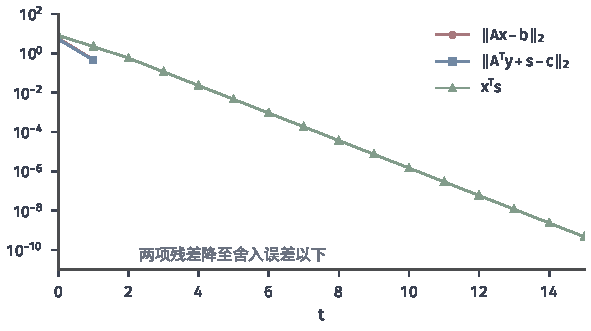
\includegraphics[width=100mm]{figures/03-optimization-evolution-and-signals/01-optimization/matplotlib/c5-pdipm/figure.pdf}
  \caption{一个资源分配线性规划（标准型$n=4$、$m=2$）上的原始—对偶内点法，$\sigma=0.2$，起点$\bm x=2\cdot\bm1$、$\bm s=\bm1$、$\bm y=\bm0$，对数纵轴。红色为原始残差$\lVert\bm A\bm x-\bm b\rVert_2$，蓝色为对偶残差$\lVert\bm A^\top\bm y+\bm s-\bm c\rVert_2$，两者在第2步取全步长后降到$10^{-12}$以下（图中不再画出）；绿色为互补量$\bm x^\top\bm s$，按约$\sigma$的比率几何下降。}
  \label{fig:opt-con-pdipm}
\end{figure}

这个例子也说明为什么三项残差都要监测。第1步后$\bm c^\top\bm x\approx-6.88$，已经低于最优值$-6.67$，因为此时$\bm x$还不满足等式约束；只看互补量或目标值会误判。只有在原始与对偶残差都足够小时，$\bm x^\top\bm s$才近似等于原始—对偶间隙$\bm c^\top\bm x-\bm b^\top\bm y$，才能作为目标误差的证书；两侧都不可行时，互补量单独不是任何误差的上界。实际报告应同时给出三项残差及所用的尺度。

改进方向选择的一种常见做法是预测—校正：先解一次$\sigma=0$的方程组（预测步），观察纯牛顿方向能把互补量降多少，据此自适应地选择$\sigma$，再加入二阶校正项解第二次（两次共用同一个矩阵分解）。这类策略在实践中显著减少迭代次数\scite{math-nocedal2006numerical}，但这是对具体实现的经验观察，不能推广为所有内点法共有的性质。

\section{半正定松弛与原解恢复}
\label{sec:opt-con-sdp-relaxation}

前面的算法大多依赖凸性：KKT条件的充分性、强对偶、内点法的中心路径，都在凸问题上才有完整的保证。许多实际问题却是非凸的二次问题，例如变量只能取$\pm1$的划分问题。本节研究一种把这类问题转成前面已经会解的半正定规划的办法：先把变量“提升”成矩阵，使二次式变成线性式，再删去唯一非凸的约束，得到一个凸的松弛问题；松弛解给出原最优值的界，但不一定是原问题的解，还需要恢复成原问题的可行候选并检验。这里改变的是候选的表示与可行集合，求解既定半正定规划的算法沿用第~\ref{sec:opt-con-interior-point}节。

\subsection{二次模型的提升与松弛}
\label{sec:opt-con-lifting}

\paragraph{精确提升}
考虑二次目标与二次约束的问题
\begin{equation}
\label{eq:opt-con-qcqp}
  \min_{\bm x\in\mathbb R^d}\ \bm x^\top\bm Q_0\bm x+2\bm q_0^\top\bm x+r_0\quad\text{s.t.}\quad\bm x^\top\bm Q_i\bm x+2\bm q_i^\top\bm x+r_i\leq0\ (i=1,\dots,m),
\end{equation}
其中$\bm Q_i$对称但不必半正定，问题一般非凸。关键观察是$\bm x^\top\bm Q\bm x=\langle\bm Q,\bm x\bm x^\top\rangle$：若引入矩阵变量$\bm X=\bm x\bm x^\top$，每个二次式都变成关于$(\bm x,\bm X)$的线性式$\langle\bm Q_i,\bm X\rangle+2\bm q_i^\top\bm x+r_i$。为了把$\bm x$与$\bm X$绑在一起，使用块矩阵
\[
  \bm Y=\begin{bmatrix}1&\bm x^\top\\\bm x&\bm X\end{bmatrix}\in\mathbb S^{d+1}.
\]
若$\bm X=\bm x\bm x^\top$，则$\bm Y=(1,\bm x^\top)^\top(1,\bm x^\top)$是半正定的秩一矩阵。反过来，若$\bm Y\succeq\bm0$、$\operatorname{rank}\bm Y=1$且左上角为$1$，则$\bm Y=\bm v\bm v^\top$，$v_1^2=1$；不妨$v_1=1$（否则把$\bm v$取负），于是$\bm x$等于$\bm v$的其余分量，$\bm X=\bm x\bm x^\top$。所以问题~\eqref{eq:opt-con-qcqp}精确地等价于关于$\bm Y$的线性目标、线性约束，加上$\bm Y\succeq\bm0$与$\operatorname{rank}\bm Y=1$。半正定与秩一两个条件共同保证新变量来自同一个原变量；非凸性全部集中到了秩一约束上。

\paragraph{删去秩一约束}
删去$\operatorname{rank}\bm Y=1$，保留$\bm Y\succeq\bm0$与左上角为$1$，就得到原问题的\term{半正定松弛}（semidefinite relaxation），它是一个半正定规划。由Schur补（引理~\ref{lem:opt-con-schur}），$\bm Y\succeq\bm0$等价于$\bm X-\bm x\bm x^\top\succeq\bm0$：松弛允许$\bm X$比真实乘积$\bm x\bm x^\top$“大”一个半正定矩阵。每个原可行点$\bm x$按$\bm X=\bm x\bm x^\top$映入松弛的可行域，且目标值不变，所以松弛的可行域包含原问题的全部候选，松弛最优值是原最优值的下界（对最大化问题则是上界）。

\begin{example}[最大割的半正定松弛]
\label{ex:opt-con-maxcut}
给定无向图的顶点$1,\dots,n$与边权$w_{a,b}\geq0$，把顶点分成两组，最大化跨组边的权重和，称为\term{最大割}（maximum cut）问题。用$x_a\in\{\pm1\}$表示顶点所在的组，边$(a,b)$跨组时$(1-x_ax_b)/2=1$，否则为$0$。约束$x_a\in\{\pm1\}$就是二次等式$x_a^2=1$。问题为
\[
  \max_{\bm x}\ \sum_{(a,b)\in E}w_{a,b}\frac{1-x_ax_b}{2}\quad\text{s.t.}\quad x_a^2=1.
\]
这里没有一次项，可直接用$\bm X=\bm x\bm x^\top$提升：目标变为$\sum w_{a,b}(1-X_{a,b})/2$，约束变为$X_{a,a}=1$。删去秩一约束，松弛为$\max\sum w_{a,b}(1-X_{a,b})/2$、$X_{a,a}=1$、$\bm X\succeq\bm0$。

取三角形图（三条边，权重均为$1$）。任何划分都至多切断两条边，最大割为$2$。松弛中，$\bm X\succeq\bm0$蕴含$\bm1^\top\bm X\bm1=3+2(X_{1,2}+X_{1,3}+X_{2,3})\geq0$，于是目标$\frac12(3-\sum X_{a,b})\leq\frac12(3+\frac32)=\frac94$；取全部非对角元为$-\frac12$，$\bm X=\frac32\bm I-\frac12\bm1\bm1^\top$的特征值为$0,\frac32,\frac32$，可行且达到$\frac94$。松弛值$9/4$严格大于真实最优值$2$，松弛解的秩为$2$，不对应任何$\pm1$向量。
\end{example}

\paragraph{与线性松弛的比较}
第~\ref{chap:opt-linear-programming}章的线性规划松弛把整数变量放宽到区间，同样扩大了候选集合、给出单侧的界。两者回答的是同一类问题，代价却不同：线性松弛保留$n$个变量，半正定松弛引入$O(n^2)$个矩阵元素和一个半正定约束，求解需要第~\ref{sec:opt-con-barrier-method}小节中代价较高的矩阵牛顿系统。对二次目标与$\pm1$变量，半正定松弛的界往往比简单的线性松弛紧，但更紧的界不意味着更低的计算成本；问题规模大时，存储和分解$\bm X$可能成为瓶颈。

也有松弛恰好精确的情形。例~\ref{ex:opt-con-sdp-eigen}中的$\min\langle\bm C,\bm X\rangle$、$\operatorname{tr}\bm X=1$、$\bm X\succeq\bm0$，正是非凸问题$\min\bm x^\top\bm C\bm x$、$\lVert\bm x\rVert_2^2=1$的半正定松弛；松弛最优解$\bm v\bm v^\top$秩为一，松弛值等于原最优值$\lambda_{\min}(\bm C)$。

\subsection{解的恢复与结果检验}
\label{sec:opt-con-rounding}

\paragraph{秩一时直接提取}
若松弛的最优解满足秩一条件，就可以按上一小节的论证提取$\bm x$：对$\bm Y$作特征分解，取最大特征值$\sigma_1$对应的单位特征向量$\bm v$，令$\bm x$为$\sqrt{\sigma_1}\bm v$缩放到首分量为$1$后的其余分量；然后逐条核对原约束~\eqref{eq:opt-con-qcqp}。数值求解给出的$\bm Y$只是近似秩一（第二大特征值很小但不为零），这时提取出的$\bm x$可能有微小违约，也必须按原约束检查。图~\ref{fig:opt-con-sdp-rounding}(a)是一个秩一的例子：四个顶点的圈（边$12,23,34,41$，权重为$1$）是二部图，最大割为$4$；松弛目标$\sum(1-X_{a,b})/2\leq4$（因为$X_{a,b}\geq-1$），而$\bm x=(1,-1,1,-1)^\top$的$\bm x\bm x^\top$达到$4$，所以松弛精确，解为秩一。

\paragraph{高秩时的随机舍入}
一般的松弛解秩大于一，需要针对任务设计恢复规则。最大割有一个经典的\term{随机超平面舍入}（random hyperplane rounding）方法。把松弛解分解为$\bm X=\bm V^\top\bm V$，$\bm V$的第$a$列$\bm v_a$是单位向量（因为$X_{a,a}=1$），$X_{a,b}=\langle\bm v_a,\bm v_b\rangle$。随机取一个方向$\bm r$（如标准正态向量），令$x_a=\operatorname{sign}\langle\bm r,\bm v_a\rangle$，即用过原点、以$\bm r$为法向的超平面把这些向量分成两组。两个单位向量被分开的概率等于它们的夹角除以$\pi$，所以舍入得到的割值期望为
\[
  \mathbb E\Bigl[\sum_{(a,b)\in E}w_{a,b}\frac{1-x_ax_b}{2}\Bigr]=\sum_{(a,b)\in E}w_{a,b}\frac{\arccos X_{a,b}}{\pi}.
\]
在非负权重下，Goemans与Williamson证明这个期望不低于松弛值的$0.878$倍，因而也不低于最大割的$0.878$倍\scite{goemans1995maxcut}。这是针对最大割的结论，依赖目标的特殊形式；不能预设任意二次问题都有保证精度的恢复办法。

回到三角形：$X_{a,b}=-\frac12$对应三个在平面内两两成$120^\circ$的单位向量（图~\ref{fig:opt-con-sdp-rounding}(b)）。每条边被分开的概率为$(2\pi/3)/\pi=\frac23$，期望割值为$3\times\frac23=2$。实际上，任何不经过这三个向量的超平面都恰好把其中一个与另外两个分开，每次舍入都得到割值$2$，正是最大割。

\begin{figure*}[!htbp]
  \centering
  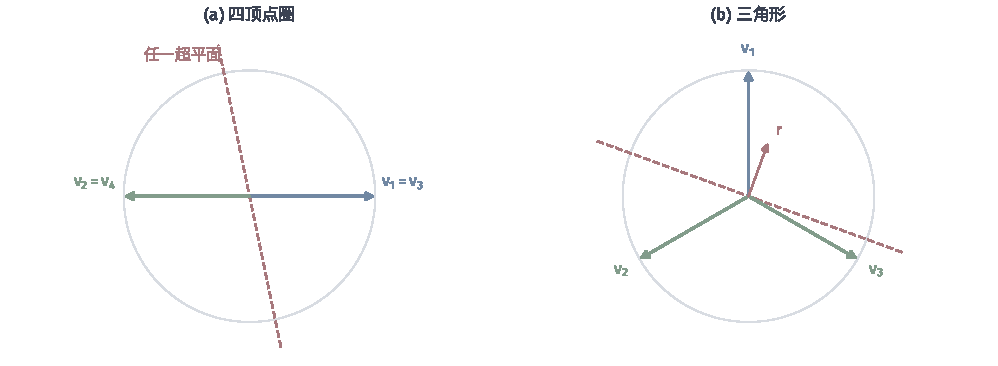
\includegraphics[width=169mm]{figures/03-optimization-evolution-and-signals/01-optimization/matplotlib/c5-sdp-rounding/figure.pdf}
  \caption{最大割半正定松弛的向量表示$X_{a,b}=\langle\bm v_a,\bm v_b\rangle$。(a) 四顶点圈：松弛解是秩一的，$\bm v_1=\bm v_3$与$\bm v_2=\bm v_4$方向相反，任何超平面（红色虚线）都给出割值$4$，与松弛值相等。(b) 三角形：三个单位向量两两成$120^\circ$，松弛值为$9/4$；以随机方向$\bm r$为法向的超平面把$\bm v_1$（蓝）与$\bm v_2,\bm v_3$（绿）分开，得到割值$2$，即最大割。}
  \label{fig:opt-con-sdp-rounding}
\end{figure*}

\paragraph{用上下界报告结果}
恢复步骤只产生候选。对实际得到的原始可行候选，其目标值给出最大割的一个下界（最大化问题）；松弛给出上界。二者合起来报告一个区间：三角形的最大割位于$[2,9/4]$，舍入候选的值$2$恰为下端点，区间宽度反映的是松弛本身的间隙，而不是舍入的损失。

这里的上界要可信。数值求解松弛问题只得到近似解，近似解的目标值可能略高或略低于真正的松弛最优值，直接拿来当上界并不严格。可靠的做法是给出一个对偶可行点。对最大割，目标可写成$\frac14\langle\bm L,\bm X\rangle$，其中$\bm L$是图的Laplace矩阵（对角元为加权度数，非对角元为$-w_{a,b}$）；对任何$\bm X\succeq\bm0$、$X_{a,a}=1$，$\frac14\langle\bm L,\bm X\rangle\leq\frac14\lambda_{\max}(\bm L)\operatorname{tr}\bm X=\frac n4\lambda_{\max}(\bm L)$。三角形的$\bm L=3\bm I-\bm1\bm1^\top$，$\lambda_{\max}=3$，上界$\frac34\cdot3=\frac94$，与松弛值一致。这类由对偶可行点构造的界，不受松弛求解误差的影响。

最后，三种误差应分别记录：求解松弛问题的数值误差（由松弛问题自身的原始—对偶残差控制）；松弛间隙，即放宽可行域造成的松弛值与原最优值之差（三角形中为$1/4$，四顶点圈中为零）；以及恢复的损失或失败，包括恢复候选违反原约束、需要修复，或目标值低于原最优值。三者来源不同，不能互相抵消或替代。最终的输出必须回到原始的非凸问题：一个经过原约束检验的候选，以及一个注明来源的界。

\section{本章小结}
\label{sec:opt-con-summary}

章首的预算分配例可以把全章串起来。最优点$\bm x^\star=(3/2,1/2)^\top$的梯度不为零，但负梯度落在可行域的法锥中；由于约束仿射、目标凸，乘子$\lambda_1^\star=1/2$与$\bm x^\star$一起满足KKT条件，这已证明全局最优。同一个乘子给出对偶下界：$q(1/2)=1/4=f(\bm x^\star)$，间隙为零，任何人都可以用这一对数据核验结果。它也回答了预算变化的问题：预算增加$0.1$，最优值至多下降$\lambda_1^\star\times0.1=0.05$，实际下降$0.0475$；在活动集不变的区间内，乘子就是最优值对预算的导数。求解方面，这个问题可以用投影（三角形上的投影可以显式计算）、惩罚或乘子法、或者把它当作二次规划用活动集法或内点法求解；它是凸问题，不需要松弛。

全章的结论可以按职责归纳。最优条件刻画候选：变分不等式只用可行域的几何，KKT条件把它写成梯度与乘子，从局部最优推出乘子存在需要约束资格（如LICQ），而凸问题中满足KKT条件就是全局最优。对偶认证目标值：弱对偶无条件地给出下界，Slater条件等正则条件保证零间隙和乘子存在，但原始最优点是否存在仍需另证；实际报告结果时，可行上界与可信下界之差是最可靠的证书。敏感性解释模型的改变：强对偶下，乘子给出最优值的全局单侧界，只有在值函数可微处才是导数；最优解的导数需要固定活动集、严格互补以及可逆的KKT矩阵，活动集变化或解不唯一时局部描述失效。算法产生候选：表~\ref{tab:opt-con-methods}比较了各类方法依赖的结构和每轮代价。

\begin{table*}[!htbp]
  \centering\small
  \begin{tabularx}{\linewidth}{@{}lXXX@{}}
    \toprule
    方法 & 适用结构 & 每轮主要代价 & 可行性与保证 \\
    \midrule
    投影梯度 & 光滑目标，投影容易的闭凸集 & 梯度加一次投影 & 每步可行；凸时$O(1/T)$，强凸时线性收敛 \\
    条件梯度 & 光滑目标，线性子问题容易的紧凸集 & 梯度加一次线性子问题 & 每步可行；凸时$O(1/t)$，解在面内部时振荡变慢 \\
    镜像下降 & 几何非欧氏的集合（如单纯形） & 梯度加一次散度子问题 & 保持在参考函数定义域内部 \\
    二次惩罚 & 一般光滑约束 & 一个无约束子问题 & 有限罚参数下不可行；参数增大导致病态 \\
    精确惩罚 & 乘子存在或误差界成立 & 一个非光滑子问题 & 罚参数超过阈值后最小点可行 \\
    增广Lagrange & 等式约束（不等式经松弛变量） & 一个光滑子问题加乘子更新 & 固定罚参数即可收敛（凸时） \\
    ADMM & 两块可分目标、线性耦合 & 两个可分子问题加乘子更新 & 残差、目标值与乘子收敛（凸时）；适合中等精度与分布式 \\
    SQP & 光滑非线性约束 & 一个二次规划 & 解附近二次或超线性收敛；需评价函数保证全局行为 \\
    内点法 & 线性规划与锥规划 & 一个KKT线性系统 & 迭代严格可行或残差逐步消除；间隙由障碍参数控制 \\
    \bottomrule
  \end{tabularx}
  \caption{本章约束优化方法的比较。表中“保证”只概括正文已说明的结论及其前提，具体条件见相应小节。}
  \label{tab:opt-con-methods}
\end{table*}

选择方法时可以按三个问题依次判断。第一，约束是什么类型：凸集上投影或线性子问题是否便宜，约束是否非线性，是否有矩阵约束。第二，子问题代价多少：一次投影、一次线性最小化、一个无约束问题、一个二次规划，还是一个KKT线性系统。第三，需要什么精度和证书：低到中等精度、需要分布式计算时，一阶方法与ADMM合适；需要高精度和原始—对偶证书时，内点法与SQP更合适。

最后要区分等价建模与松弛。把凸二次规划写成二阶锥规划、用Schur补把平方约束写成矩阵不等式，都是等价改写，最优值与最优解不变。半正定松弛则扩大了可行集合，它给出原最优值的单侧界，松弛解还必须恢复成原问题的候选并按原约束检验。在报告结果时，模型数据的敏感性、算法的计算误差、松弛的间隙与恢复的损失，应当分别说明来源和大小。

